\documentclass[11pt, twoside]{report}
\usepackage[utf8]{inputenc}
\usepackage[toc, page]{appendix}
\usepackage{amsmath}
\usepackage{graphicx}
\usepackage[margin=1in]{geometry}
\usepackage{placeins}
\usepackage{setspace}
\usepackage[acronym]{glossaries}
\usepackage{url}
\graphicspath{ {images/} }
\usepackage{geometry}
\usepackage{dirtytalk}
\usepackage{multirow}
\usepackage[table]{xcolor}
\usepackage{type1cm}
\usepackage{lettrine}
\usepackage{listings}
\usepackage{algorithm}
\usepackage{algpseudocode}

\geometry{
	legalpaper, 
	portrait,
	total={297mm, 210mm},
	top = 25mm, 
	bottom = 25mm, 
	left = 40mm, 
	right = 20mm
	}

\linespread{1.5}

\usepackage[epsilon, altpo]{backnaur}


\title{
{\huge \textbf{Procedural Plant Generation and Simulated Plant Growth }}\\
\vspace{3cm}
{\large A thesis presented in partial fulfilment of the requirements for the degree of \\
\vspace{4cm}
\large \textbf{Master of Information Science}\\
\large \textbf{in}\\
\large \textbf{Computer Science}\\
\vspace{4cm}
\large at Massey University, Albany, \\
\large New Zealand. }
\vspace{3cm}
\author{Matthew Halen Crankshaw}
\date{2019}
}

\makeglossaries
\newglossaryentry{C/C++}
{
	name=C/C++, 
	description={Refers to the C and C++ programming languages}
}

\newglossaryentry{OpenGL}
{
	name=OpenGL, 
	description={The Open Graphics Library is a cross-platform, cross-language application programming interface used in creating graphics applications}
}

\newglossaryentry{Lexer}
{
	name=lexer, 
	description={A computer program that performs lexical analysis}
}

\newglossaryentry{Parser}
{
	name=parser,
	description={A computer program that performs parsing}
}

\newglossaryentry{Morphology}
{
	name=morphology, 
	description={The study of the forms of things}
}

\newglossaryentry{Shader}
{
	name= shader, 
	description={A set of instructions that run on the graphics processing unit which calculates rendering effects}
}

\newacronym{2d}{2D}{Two Dimensional}
\newacronym{3d}{3D}{Three Dimensional}
\newacronym{api}{API}{Application Programming Interface}
\newacronym{bnf}{BNF}{Backus-Naur Form}
\newacronym{cfg}{CFG}{Context-Free Grammar}
\newacronym{cpu}{CPU}{Central Processing Unit}
\newacronym{eol}{EOL}{End of Line}
\newacronym{eof}{EOF}{End of File}
\newacronym{glm}{GLM}{OpenGL Mathematics Library}
\newacronym{glsl}{GLSL}{OpenGL Shading Language}
\newacronym{gpu}{GPU}{Graphics Processing Unit}
\newacronym{opengl}{OpenGL}{Open Graphics Library}
\newacronym{stl}{STL}{Standard Template Library}
\newacronym{glfw}{GLFW}{Graphics Library Framework} 
\newacronym{lerp}{LERP}{Linear Interpolation}
\newacronym{lifo}{LIFO}{Last In First Out}
\newacronym{flex}{Flex}{Fast Lexical Analyzer Generator}
\newacronym{vao}{VAO}{Vertex Array Object}
\newacronym{vbo}{VBO}{Vertex Buffer Object}

\begin{document}

\maketitle

\chapter*{Acknowledgements}

I would like to start by thanking my supervisor Dr Daniel Playne., for all of your support, guidence and feedback during the course of this thisis, additionally I would like to acknowledge Dr Martin Johnson. You both have an immense knowledge and passion for computer science and your students that is awe inspiring.\\
\\
\noindent
A very special gratitude goes to my colleagues Dara and Richard in the center for parallel computing for their assistance and friendship. \\
\\
\noindent
I certainly would not be where I am today if it weren't for my siblings, mother and father for their continued love and support.\\
\\
\noindent
Finally, to my beloved partner Romana, thank you for your unwaivering support and encouragement throughout the last year of study, and in the writing process or this thesis. This accomplishment would not be possible without you. 


\chapter*{Abstract}

The procedural generation and simulation of realistic looking plant-life assets in 3D applications is a challenging task. Research has shown that the L-systems' rewriting mechanism is an effective means for procedurally generating structures that represent multiple types of plant-life, those structures can be interpreted as a set of instructions to render a realistic model. This study aims to investigate the relationship between the rewriting mechanism of the L-system and the way that the resulting structure is interpreted and rendered on the screen, and to determine if an L-system can manipulate the physical properties of branches to provide the relevant information needed to physically simulate a plants reaction to wind and gravity. 

After a review of the literature, a parametric L-system was developed, that can create plant structures that have variation in their branching structure and physical features, and that are capable of holding the parameters for a physical simulation. A system for representing and simulating the result generated by the rewriting system was implemented and tested on L-systems of varying complexity. The results show that an L-system can be created not only to represent a plants structure but also its physical properties, with the dissadvantage that the L-system becomes more cumbersome and difficult to understand. On this basis, it is beneficial to have a plant assets that not only are procedurally generated but also can be easily simulated.

\tableofcontents
\listoffigures
\listoftables


\chapter{Introduction}

\lettrine[lines=3]{P}{}rocedurally generating 3D models of plant-life is a challenging task, largely due to the complex branching structures and variation between different types of plant species. Up until recently, all assets within 3D graphics applications either had to be sculpted using 3D modeling software, or scanned using photogrammetry, laser triangulation or some form of contact based 3D scanning. These methods are still used today but tend to be very time consuming and extremely costly. With the increase in computational power over the last few decades more emphasis has been placed on the use of produral generation. Which can be used to create complex structures such as terrain, architecture, sound and 3D models with far greater speed than previous techniques, and often much better realism than would be possible with artists. Plant-life stands as a challenge due to the thousands of species, each with their own unique structure and features. It is difficult to define a system that can represent them all in a way that is simple, understandable and accurate. The Lindenmayer System (L-system) stands as a solution to this problem, it was originally developed by Aristed Lindenmayer as a method of representing the development of multicellular organisms \cite{lindenmayer1968mathematical}. This has since gained popularity in the area of procedural generation and has been adapted to represent different types of structures. L-systems have been adapted to represent plant-life, such as trees, flowers, algea and grasses, whilst still being applicable to non-organic structures such as music, artificial neural networks and tiling patterns \cite{Prusinkiewicz1989}.\\

The L-system in its most basic form, is a formal grammar which contains a set of symbols or letters that belong to an \textit{alphabet}. The alphabet is used to create a starting string known as the \textit{axiom}, as well as a set of production rules. The production rules are applied to each symbol within the axiom string, each rule dictates whether or not the symbol can be rewritten and furthermore, what they will be rewritten with. In essence, a L-system uses the set of production rules to generate a resulting string of symbols which follow those production rules. The resulting strings' meaning can then be interpreted in a way that best fits what it is trying to represent. In this case the string can interpreted to generate a model of a plant. This thesis develops upon the L-system concepts described by Przemyslaw Prusinkiewicz and Aristid Lindenmayer to procedurally generate structures of plant-life in real-time. The L-system grammar allows the structure of a plant to be described in a human readable, formal grammar. The grammar can be used to specify variation in shape, size and branching structure within a particular species. Furthermore, this thesis will also investigate the use of a parameterised L-systems to provide physical properties using string rewriting. Which in turn will enable the animation and physical behaviour of the plant that it generates, thus making it possible to simulate external forces such as gravity and wind.\\

This chapter will describe the motivations behind this research and how it can be used to improve the procedural generation of plant-life in 3D applications. It will then introduce the concepts of procedural generation, rewriting systems and formal grammars. Briefly describing how procedural generation can be applied to the development of plant-life through the use of rewriting systems. Furthermore, this chapter will provide sufficient background as to the use of formal grammars as a means of describing complex L-system languages. Finally there will be an outline as to the structure of this thesis, and how this research will be conducted.

\section{Motivations}

L-systems have been talked about and researched since its inception in 1968 by Aristid Lindenmayer. Over the years it's usefulness in modeling different types of plant life has been very clear, however its presence has been quite absent from any mainstream game engines and graphics applications for the most part, these engines relying either on digital artists skill to develop individual plants or on 3rd party software such as SpeedTree. These types of software use a multitude of different techniques however their methods are heavily rooted in Lindenmayer Systems. 
 
One of the most time consuming parts for digital artists and animators is creating differing variations of the same piece of artwork. In most games and other graphics applications environment assets such as trees, plants, grass, algae and other types of plant life make up the large majority of the assets within a game, and creating a plant asset can take a skilled digital artist more than an hour of work by hand, The artist will often have to create many variations of the same asset in order to obtain enough variation that a user of that graphics application would not notice that the asset has been duplicated, if this is multiplied by the number of assets that a given artist will have to create or modify, there is an incredible number of hours that could have potentially been put to use creating much more intricate assets. In addition to this, it is also important to note that graphics assets are then stored in large data files, describing the geometry and textures and other information. If we require three very similar plants, we have to store three separate sets of data. Procedurally generating plants can avoid this wasteful data storage entirely, instead a relatively small L-system description can be stored which can be used to procedurally generate all the required geometry and other information during the execution of the program.\\

The L-system can not only procedurally generate the geometry of the plant-life but can also generate parameters physical properties of the plant inself such as the weight and flexibility of branches as well as its wind resistance and many other important information that can be used to simulate or animate the motion of the plant under various forces.  

\section{Introduction to Procedural Generation}

Procedural generation is used in many different areas and applications in computer graphics, particularly when generating naturally occuring structures such as plants or terrain. An effective procedural generator is capable of taking input in the form of a relatively simple description of what it should be generating, its job is then to computationally generate the structure in a way that is accurate to the description given. Currently there are three main methods for procedurally generating models of plant-life, these are genetic algorithms \cite{haubenwallner2017shapegenetics}, space colonisation algorithms\cite{juuso2017procedural} and L-systems. The genetic algorithm and space colonisation algorithms are similar in that they require the overall shape of the plant to be described by simple 3D shapes, the algorithm then creates a branching structure that matches these shapes. The limitation of these methods is that the 3D description is not very specific and although it can get good results for trees, it may not be able to generate a different types of plant-life, such as flowers. The L-system on the other hand relies on a mothod of string rewriting, whereby the rewriting is based on a set of production rules in order to generate a string of symbols that obay those rules. A separate system can later interpret this string to create the model. The L-system procedural generation therefore, has two separete systems within it, one of string rewriting and one of interpretation of the generated string. This makes it quite easy for the same L-system to generate very different results based upon the interpretation.\\

Plant-life can have very complex and seemingly random structures, however, with closer observation, trees of a similar species have obvious traits and features. For instance, a palm tree has long stright trunks with long compound leaves exclusively near the top, branching in all different directions. Comparatively a pine tree has a long staight trunk with many branches coming off in different directions pupendicular to the ground, from its base to the top of the trunk. These are two very different species of trees, the palm  belongs to the Arecaceae family, whereby the pine belongs to the Pinaceae family. They look different, however, they share very similar properties, such as their long straight trunks. The challenge behind the  procedural generation of plant-life, is providing a human readable grammar that describes in sufficient detail, how to generate a three dimensional model. Whilst allowing for randomness and variety within the generation process, such that variations of a particular species can be generated without repetition. The  grammar for procedural generation should also be relatively straightforward and intuitive, and must accurately represent what it is going to generate. Furthermore, the description must not be limited to only known species of trees, as some graphics applications may require something that is other-wordly.

\section{Introduction to Rewriting Systems}

Rewriting systems are the fundamental concept behind L-systems. In their most basic form, rewrite systems are a set of symbols or states, and a set of relations or production rules that dictate how to transform from one state to the other \cite{prusinkiewicz2012algorithmic}. Using these state transitions it is possible to generate complex structures by successively replacing parts of a initial simple object with more complex parts. Rewrite systems can be non-deterministic, meaning that there could be a transition which depends on a condition being met or on a neighbouring states. Using this rewriting concept any preceeding state can rely upon some conditions neccessary for transformation. If condition is true the state will be rewritten, otherwise it will remain the same, and will be checked in the next rewriting stage. A graphical representation of an object defined in rewriting rules can be seen below in figure \ref{snowflake curve} below, called the snowflake curve proposed by Von Koch \cite{koch1906methode}.

\begin{figure}[htbp]
	{\centering
		\setlength{\fboxrule}{1pt}
		\vspace{7px}
		\fbox{
			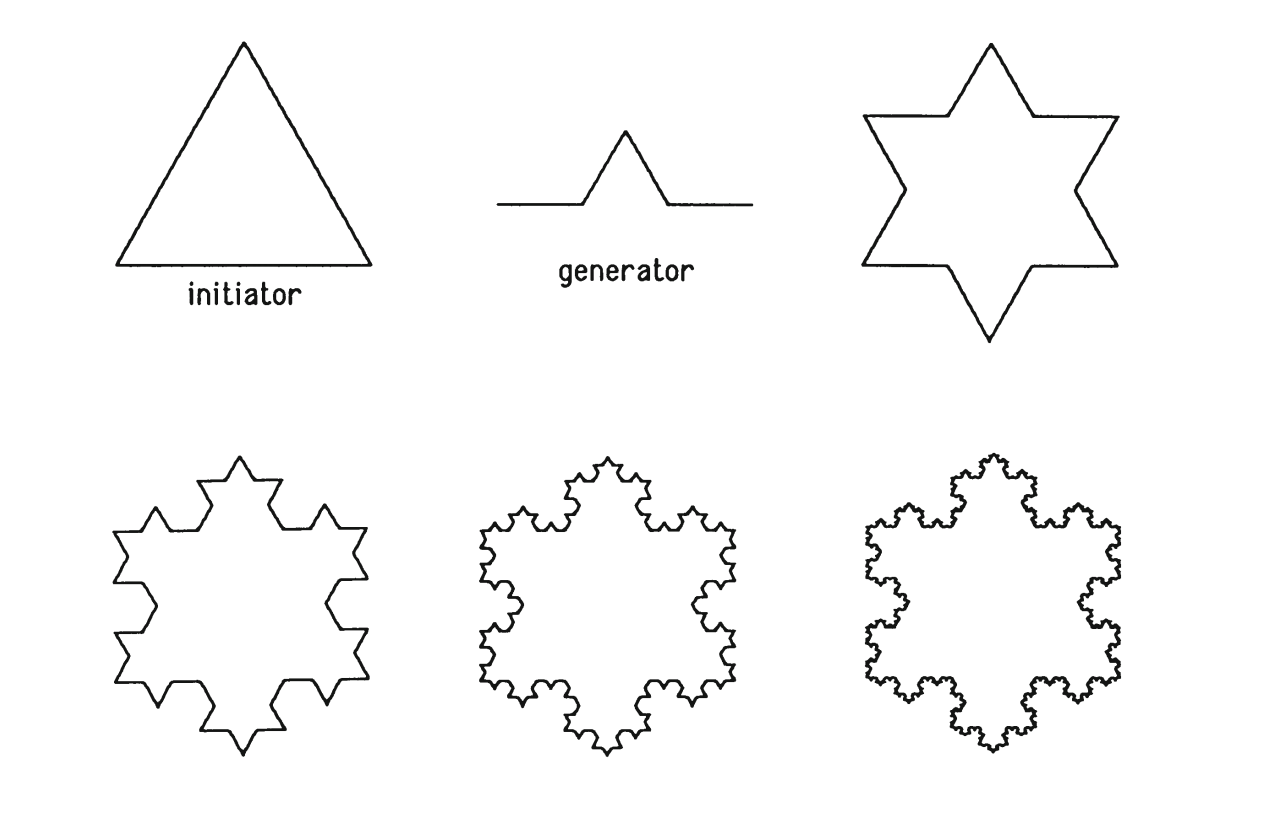
\includegraphics[scale=0.3]{Diagrams/snowflakeCurve.png}
		}
		\caption{Construction of the snowflake curve\cite{prusinkiewicz2013lindenmayer}.} \label{snowflake curve}
	}
\end{figure}
\FloatBarrier

\noindent
The snowflake curve starts with two parts, the initiator and the generator. The initiator is is the initial set of edges forming a certain shape, whereas the generator is a set of edges which can be used to replace each edge of the initiator to form a new shape. That new shape then becomes the initiator for the next generation, where each edge is again replaced by the generator. The result is a complex shape similar to that of a snowflake. The initiator, generator concept is a graphical representation of how rewriting systems operate, rather than the initiator and generator being a set of edges they are instead represented by a set of symbols or strings.

\section{Introduction to Formal Grammars}

In the context of computer science, grammars are defined as a set of rules governing which strings are valid or allowable in a language or text. They consist of syntax, morphology and semantics. Formal languages have been defined in the form of grammars to suit particular problem domains. It is natural for humans to communicate a problem or solution in the form of language, it is therefore intuitive to use a language to describe the desired outcome when dealing with the procedural generation of plant-life. In the past, formal grammars have been used extensively in computer science in the form of programming languages in which humans can provide a computer with a set of instructions to carry out in order to gain an expected result. The challenge is therefore to create a  grammar in the form of a rewriting system that facilitates the procedural generation of plant-life. A rewriting system such as the L-system operates in a way that is consistant with a context-free class of Chomsky grammar \cite{chomsky1956three}, similar to that of the programming language ALGOL-60 introduced by Backus and Naur in  1960\cite{backus1960report}. In figure \ref{chomsky grammars} below, there are two types of L-system grammars that overlap the classes of chomsky grammars, the OL-system and the 1L-system. The details of these two systems will be discussed in detail chapter \ref{l-system chapter}, but in summary, 0L-systems are grammars that can represent a context-sensitive Chomsky grammar but generally tend to be context-free, the main difference between the 0L-system and the 1L-system is that 1L-systems can be recursively enumerable. Furthermore, it is possible for a 1L-system to represent any 0L-system, therefore, 1L-system languages tend to be more complex and verbose when compared to 0L-systems, this creates a trade off between a more powerful and complex language or a less powerful but simpler language. 

\begin{figure}[htbp]
	{\centering
		\setlength{\fboxrule}{1pt}
		\vspace{7px}
		\fbox{
			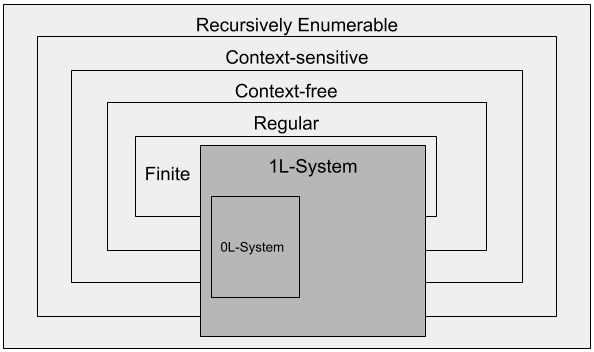
\includegraphics[scale=0.5]{Diagrams/ChomskyGrammar.png}
		}
		\caption{Diagram of the Chomsky hierarchy grammars with relation to the 0L and 1L systems generated by L-systems.} \label{chomsky grammars}
	}
\end{figure}
\FloatBarrier

\section{Structure of Thesis}

This thesis begins by delving into the underlying concept of L-systems. This starts by defining the simplest type of L-system named the DOL-system, it also goes into detail about how they can be interpreted to produce a graphical representation. This will lead into the formal definition of more complex types of L-systems such as the parametric L-system, of which this thesis mainly focuses on. In conjunctio with this, some of the major features and improvements which can be used to aid the production of plant life will be described in detail. 

The next major part of the thesis will focus on the L-system rewriter implementation, this includes the definition of the grammar and syntax for a parametric L-system language. This talks about the process of string rewriting, including computationally understanding the L-system grammar using lexical analysis, parsing and the string rewriting algorithm definition. This rewriter implementation will also delve into some of the systems of specifics of how rewriting works and its connection to string interpretation.

The next two chapters cover some specific mathematics concepts necessary for 3D graphics, such as vectors, matrix transformations and quaternions. The mathematics section leads into the physics chapter which focuses on the physics behind the simulation of 3D generated plants. This includes details of Hook's Law and the equations of motion. As well as how these calculations can be acieved within a 3D application.

Chapter \ref{interpreter implementation} discusses the three main stages of L-system string interpretation with regards to generating 3D plant-life. These three stages are the turtle graphics interpreter, model generator and renderer. The turtle graphics interpreter goes into detail about how the skeletal and joint structure of plants work. The model generate talks about how the skeletal structure can be used to generate a 3D model of the plant that represents a realistic looking plant. Finally the renderer covers the specifics of rendering models on the screen in the OpenGL framework.







\chapter{Lindenmayer Systems}  \label{l-system chapter} 

\lettrine[lines=3]{T}{}he L-system at its core is a formal grammar made up of an \textit{alphabet} of characters which are concatenated together into collections of symbols, called strings. The L-system describes a starting string called the \textit{axiom}, and a set of production rules. For each rewriting step the production rules determine whether a symbol within a string should be rewritten with another symbol or string. Each symbol within the \textit{axiom} is matched against the production rules. If a match is found, the symbol within the axiom is replaced with a predecessor string described by the production rule. This process is carried out for each symbol in the \textit{axiom}. The resulting string created by the rewriting process then becomes the axiom, which can then be rewritten once again. This process of rewriting using production rules is the mechanism for generating a structure of states that obay the production rules, similar to that of a context-free grammar. Essentially the symbols represent a particular state of the system, and the production rules decide whether that state should transition based on a certain criteria, and what the next state should be. 

This chapter will discuss a number of different types of L-systems, as well as their features and limitations. It will focus on the mechanics behind the rewriting system and different techniques that can be used to better represent plant-life as an L-system. In order to provide sufficient background, this chapter will also touch briefly on how the resulting strings generated by the L-system can be interpreted. The interpretation of an L-system is a separate system to the L-system, however, it is important to note that the L-system itself has no concept of what it is trying to represent, it is simply a string rewriting system. The L-systems interpretation is left up to a separate system, responsible for interpreting the resulting string to create a suitable representation for that problem domain. For instance, the symbols for a L-system trying to represent a tree, may be interpreted very differently to the symbols trying to represent music, however, the L-systems may be identical. Although the interpreter is not neccessarily part of the L-system it is an important to understand the reliance of the L-system on the string interpreter. The string interpreter will be in great detail in chapter \ref{interpreter implementation}.


A well-known biologist, Aristid Lindenmayer, started work on the Lindenmayer System or L-system in 1968, he sought to create a new method of simulating the growth in multicellular orgamisms such as algae and bacteria \cite{lindenmayer1968mathematical}. He later defined a formal grammar for simulating multicelular growth which he called the 0L-system \cite {lindenmayer1971developmental}. In the last twenty years, the concept has been adapted to be used to describe larger organisms such as plants and trees as well as other non organic structures like music \cite{worth2005growing}. There has also been studies to try to use an L-system as a method of creating and controlling growth of a connectionist model to represent human perception and cognition \cite{vaario1991connectionist}. Similarly, K{\'o}kai et al. (1999) have created a method of using a parametric L-system to describe the human retina, this can be combined with evolutionary operators and be applied to patients with diabetes who are being monitored \cite{kokai1999parametric}.


\section{Simple DOL-system} \label{Simple DOL-systems}

According to Prusinkiewicz and Hanan the most simple type of L-systems is known as the D0L-system. The term 'D0L system' abbreviates 'Deterministic Lindenmayer system with zero-sided interactions'. It is deterministic as each symbol has an associated production rule and there is no randomness in determining which rule should be chosen. A zero-sided interaction refers to the multicellular representation of an L-system, where each symbol refers to a type of cell, each cell does not account for the state of its direct neighbouring cells, making it zero-sided. There are three major parts to a D0L system. Firstly there is a finite set of symbols known as the (\textit{alphabet}), the starting string or (\textit{axiom}) and the state transition rules (\textit{rules}). The alphabet is a set of characters which represent a particular state in a system. The starting string or \textit{axiom} is the starting point of the system which contains one or more characters from the alphabet. The transition rules dictate whether a state should remain the same or transition into a different state or even disappear completely. \cite{prusinkiewicz2013lindenmayer}. 

The DOL-system was originally created to serve as a context-free grammar, to represent the development of multicellular organisms. In the DOL-system below, is an example formulated by Prusinkiwicz and Lindenmayer to simulate Anabaena Catenula which is a type of filamentous cyanobacteria which exists in plankton. According to Prusinkiewicz and Lindenmayer "Under a microscope, the filaments appear as a sequence of cylinders of various lengths, with $a$-type cells longer than $b$-type cells. The subscript $l$ and $r$ indicate cell polarity, specifying the positions in which daughter cells of type $a$ and $b$ will be produced \cite{prusinkiewicz2012algorithmic}.

\begin{equation} \label{DOL-system example}
\begin{aligned}
	&\omega~~ : a_r \\
	&p_1~ :  a_r~ \rightarrow~ a_l b_r\\
	&p_2~ :  a_l~ \rightarrow~ b_l a_r\\
	&p_3~ :  b_r~ \rightarrow~ a_r\\
	&p_4~ :  b_l~ \rightarrow~ a_l\\
\end{aligned}
\end{equation}

\noindent
With the definition above, the DOL-system states $w~ :~ a_r$, the symbol $w$ signifies that what follows is the starting point (axiom), therefore, the starting point is the cell $a_r$. The production rules then follow and are $p1, p2, p3$ and $p4$. The : symbol separates the axiom and production names from their values, furthermore the $\rightarrow$ can be verbalised as "is relaced by" or "rewritten with". In production rule 1 ($p1$) the cell $a_r$ will be rewritten with cells $a_l b_r$, $p2$ states that $a_l$ will be rewritten with cells $b_l a_r$, $p3$ states $b_r$ will rewritten with cell $a_r$ and finally production rule 4 ($p4$), states that $b_l$ will be rewritten with cell $a_l$. In order to simulate Anabaena catenula we require these four rewritting rules, as there are four types of state transitions. \\
\\
The resultant strings of five generations of the DOL-system rewritting process: 

\begin{equation} \label{DOL-system result string}
\begin{aligned}
	& G_0~ :~ a_r \\
	& G_1~ :~ a_l b_r \\
	& G_2~ :~ b_l a_r a_r \\
	& G_3~ :~ a_l a_l b_r a_l b_r \\
	& G_4~ :~ b_l a_r b_l a_r a_r b_l a_r a_r \\
	& G_5~ :~ a_l a_l b_r a_l a_l b_r a_l b_r a_l a_l b_r a_l b_r \\
\end{aligned}
\end{equation}
\noindent
During the rewriting process, generation zero ($G_0$) is the axiom. In subsequent generations the resultant string of the previous generation is taken and each symbol in the string is compared to the production rules, if they match the production rule the symbol is rewritten with the next symbol or a string that is specified by the production rule. For $G_1$ the previous generation resultant string is taken, which in this case is $G_0$, being $a_r$, the first symbol is compared with the production rules. In this case it matches rule $p1$ with the rule $p1~ :~ a_r~ \rightarrow~ a_l b_r$ and therefore, $a_r$ is rewritten with $a_l b_r$. $G_0$ only has one symbol, so it can be concluded that the string of $G_1$ is $a_l b_r$, this string is stored for the next rewriting step and is later rewritten to produce generation two and so on, until the desired number of generations is reached.

The D0L-system is very simple and minimalist in design, which comes with some limitations. The D0L-system production rules merely state that a if the symbol matches, then that symbol will be rewritten, often this is not the case, there may be some other conditions that may need to be checked before it can be concluded that a rewrite should take place. Furthermore, the symbols within a D0L-system do not supply very much information, for instance, how does the D0L-system indicate how many times a given string has been rewriten? The D0L-system is also deterministic, meaning that there is no randomness the rewriting process, therefore, it will always yield the same result with no variation.

\section{Interpreting the DOL-system} \label{Interpreting DOL-system}

Section \ref{Simple DOL-systems} outlines a simple type of L-system known as the DOL-system, this L-system specifies a set of symbols, a starting point and a set of production rules, allowing us to represent a problem as a set of states. The production rules can express valid state transisions, which thereafter allows us to produce a resultant string of symbols that obey the L-systems production rules. This functionality is powerful in and of itself, however, the L-system's symbols are only useful if they represent some kind of meaning, furthermore the L-system does not supply this meaning, each symbol's meaning is interpreted after the rewriting process of the L-system by the interpreter. Due to this, there are two separate and very different systems involved in taking an L-systems input, such as the alphabet, axiom and production rules and turning it into something that is able to model plant-life. These two systems are the L-system rewriter, which is reposponsible for using L-system to rewrite a string and provide a resultant string of symbols. The L-system interpreter takes the resultant string from the L-system rewriter and interprets it in a way that is able to represent the model we are trying to create. 

A paper by Przemyslaw Prusinkiewicz outlines a method for interpreting the L-system in a way that can model fractal structures, plants and trees. The method interprets the resultant string of the L-system, where each symbol represents an instruction which is carried out one after the other to control a 'turtle' \cite{prusinkiewicz1986graphical}. When talking about a turtle, Prusinkiewicz is referring to turtle graphics. Turtle graphics is a type of vector graphics that can be carried out with instructions. It is named a turtle after one of the main features of the Logo programming language. The simple set of turtle instructions listed below, can be displayed as figure \ref{basic turtle}. The turtle starts at the base or root of the tree and interprets a set of rotation and translation movements, which when all executed one after the other, trace the points which make up the plant structure, when these points are then joined together the result is a fractal structure such as a plant or tree.

\begin{table}[h!]
\centering
\begin{tabular}{ | c | l | }
\hline
	Instruction Symbol 	& Instruction Interpretation \\  
\hline
\hline
	F 					& Move forward by a specified distance whilst drawing a line\\
\hline
	f 					& Move forward by a specified distance without drawing a line\\
\hline
	+ 					& Yaw to the right specified angle.\\
\hline
	- 					& Yaw to the left by a specified angle.\\
\hline
	/ 					& Pitch up by specified angle. \\
\hline
	$\backslash$ 		& Pitch down by a specified angle.\\
\hline
	$\hat{}$ 			& Roll to the right specified angle.\\
\hline
	\& 					& Roll to the left by a specified angle.\\
\hline
\end{tabular}
\caption{Table of turtle instruction symbols and their meaning to the interpreter}
\label{instruction table 1}
\end{table}
\FloatBarrier

\noindent
In the OL-system there are a number of symbols that represent a particular meaning to the L-system interpreter. Whenever the interpreter comes across one of these symbols in the resultant string, it is interpreted as a particular turtle instruction which can be seen in table \ref{instruction table 1}. 

\begin{figure}[htbp]
	{\centering
		\setlength{\fboxrule}{1pt}
		\vspace{7px}
		\fbox{
			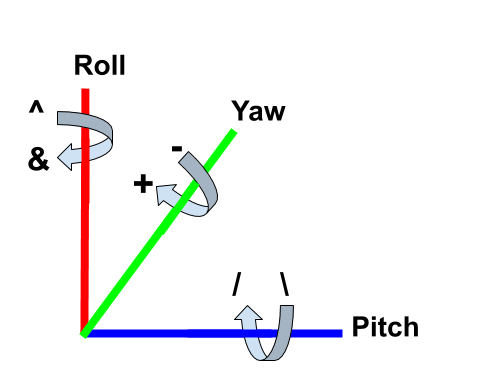
\includegraphics[scale=0.3]{Diagrams/rotations.png}
		}
		\caption{Diagram of the 3D rotations of the turtle.} \label{3D rotations}
	}
\end{figure}
\FloatBarrier

\noindent
The turtle instructions are presented in such a way that allows movement in three dimensions, the rotations in yaw, pitch and roll, where yaw is a rotation around the Z axis, pitch is rotation around the X axis and roll is rotation around the Y axis. We have two symbols for each rotation, which represent positive and negative rotations repectively. Rotations are expected to be applied before a translation, that way the rotations change the orientation of the turtle and then the forward instructions move the turtle in the Y direction using the current orientation. The orientation is maintained from translation to translation, and subsequent rotations are concatenated to maintain a global orientation, in this way when the turtle moves forward again, it will move in the direction of this global orientation. Diagram  \ref{3D rotations} shows the yaw, pitch and roll rotations as well as their axis and the instruction symbols for the L-system.\\
\\
The turtle instructions in the table \ref{instruction table 1}, can be used as the alphabet for the rewriting system in the the L-system grammar below:

\begin{equation} \label{DOL-system example}
\begin{aligned}
	&\text{Generations: 1}\\
	&\text{Angle: 90$^{\circ}$}\\
	&\omega~~ : F \\
	&p_1~ :  F~ \rightarrow~ F+F-F-F+F\\
\end{aligned}
\end{equation}

\noindent
This L-system makes use of the alphabet "F, +, -". The meaning of these symbols is not relevent to the rewriting system, so we can use the axiom and production rule to rewrite by one generation. The only piece of information which is relevant to the interpreter is the angle to rotate by when it comes across the symbols + and - this is specified in the definition of the L-system with Angle: 90$^{\circ}$. The resulting string would be "F+F-F-F+F", this string is passed to the interpreter system which uses turtle graphics to execute a list of instructions. These instructions can be articulated in the list below.

\begin{table}[h!]
\centering
\begin{tabular}{ | c | c | l | }
\hline
	 	Instruction Number & Instruction Symbol & Instruction Interpretation \\  
\hline
\hline
	I1 						& F & Move forward by 1\\
\hline
	I2						& + & Yaw right by 90 degrees\\
\hline
	I3						& F & Move forward by 1\\
\hline
	I4						& - & Yaw left by 90 degrees \\
\hline
	I5						& F & Move forward by 1\\
\hline
	I6 						& - & Yaw left by 90 degrees \\
\hline
	I7 						& F & Move forward by 1\\
\hline
	I8 						& + & Yaw right by 90 degrees\\
\hline
	I9 						& F & Move forward by 1\\
\hline
\end{tabular}
\caption{Table showing each instruction symbols and their meaning for the L-system \ref{DOL-system example}}
\label{Instruction Interpretation}
\end{table}
\FloatBarrier

\noindent
These instructions are carried out one after the other, moving the turtle around the screen in three dimensions, furthermore, tracing the structure which the 0L-system has generated, these instructions will generate the traced line shown in figure \ref{basic turtle}.

\begin{figure}[htbp]
	{\centering
		\setlength{\fboxrule}{1pt}
		\vspace{7px}
		\fbox{
			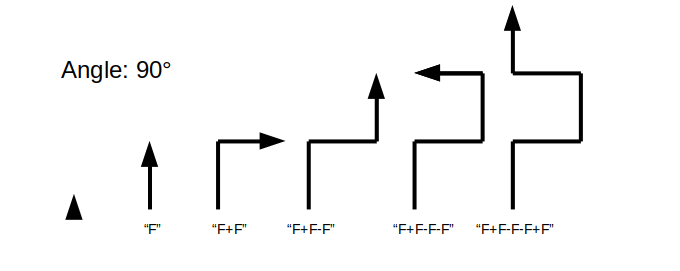
\includegraphics[scale=0.3]{Diagrams/basic_turtle.png}
		}
		\caption{Diagram showing a turtle interpreting simple L-system string.} \label{basic turtle}
	}
\end{figure}
\FloatBarrier

\noindent
As we can see from the turtle interpretation above, the turtle moves around as if it is an entity within a 3D world following a set of instructions telling it where to move. This is the basic concept of turtle graphics and how it is implemented in the interpreter system. What also becomes apparent is that there are a number of assumptions which the interpreter makes in order to produce the final image in I9. It is assumed that that the + and - symbols mean a change in yaw of 90 degrees, and the second assumption is that the F symbol means to move forward by a distance of 1 unit measurement. The angle and distance values are assumed because the resultant string does not explicitly define the angle or the distance, it leaves that up to the interpretation of the string. 

In a simple DOL-system like the one above, there is no explicit way of providing this additional information to the interpreter, as such it must be hardcoded into the interpretation, or assumed by some other means. This highlights one of the considerations when creating an L-system. There is a difference in complexities between the L-system rewriter and the interpreter. It is possible to create a very complex rewriting system with extensive rule systems, which is able to supply a large amount of information to the interpreter, the interpreter can be quite rudimentary and follow the instructions exactly. Conversely, we could have a system where the L-system rewriter is quite basic, but the interpreter is very complex and must be capable of representing the L-system despite the lack of information in the resultant string, or be able to obtain this information by other means. 

It may be tempting to leave the complexity to the interpreter in order to make the L-system rewriter and its rules more simple, however, the drawback of this, is that the information needed for modeling branch diameters, branching angles even the type of objects that need to be represented have to be supplied to the interpreter in some way, and if not through the resulting string of information, how is this information meant to provided to the interpreter. An answer may be to build a system within the interpreter that is capable of assuming the general look of a plant, for instance, branches which decrement in diameter, branching angles which are consistant and other aspects. This results in a very inflexible system which may work for a portion of plant-life but might struggle to represent certain classes of plant-life. Therefore, the benefit of using a system with most of its complexity within the rewriting system is that the L-system is responsible for some of the details of the interpretation such as angles, branch diameters and so on. In the next few sections, different types of L-systems will be discribed, explaining their benefits and limitations, as well as developing a system intergrating these separate systems into a single L-system grammar.   

There are a number of fractal geometry that have become well known particularly with regards to how they can seemingly imitate nature \cite{mandelbrot1982fractal}. Particularly with the geometry such as the Koch snowflake which can be represented using the following L-system.

\begin{figure}[htbp]
	\raggedright
	\textbf{\underline{Koch Curves:}} \\
	Generations: 2,3,4 \\
	Angle: 90$^\circ$\\
	Distance: 1 cm\\
	$\omega$ : F \\
	$p1$ : F $\rightarrow$ F+F-F-F+F\\
	{\centering
		\vspace{7px}
		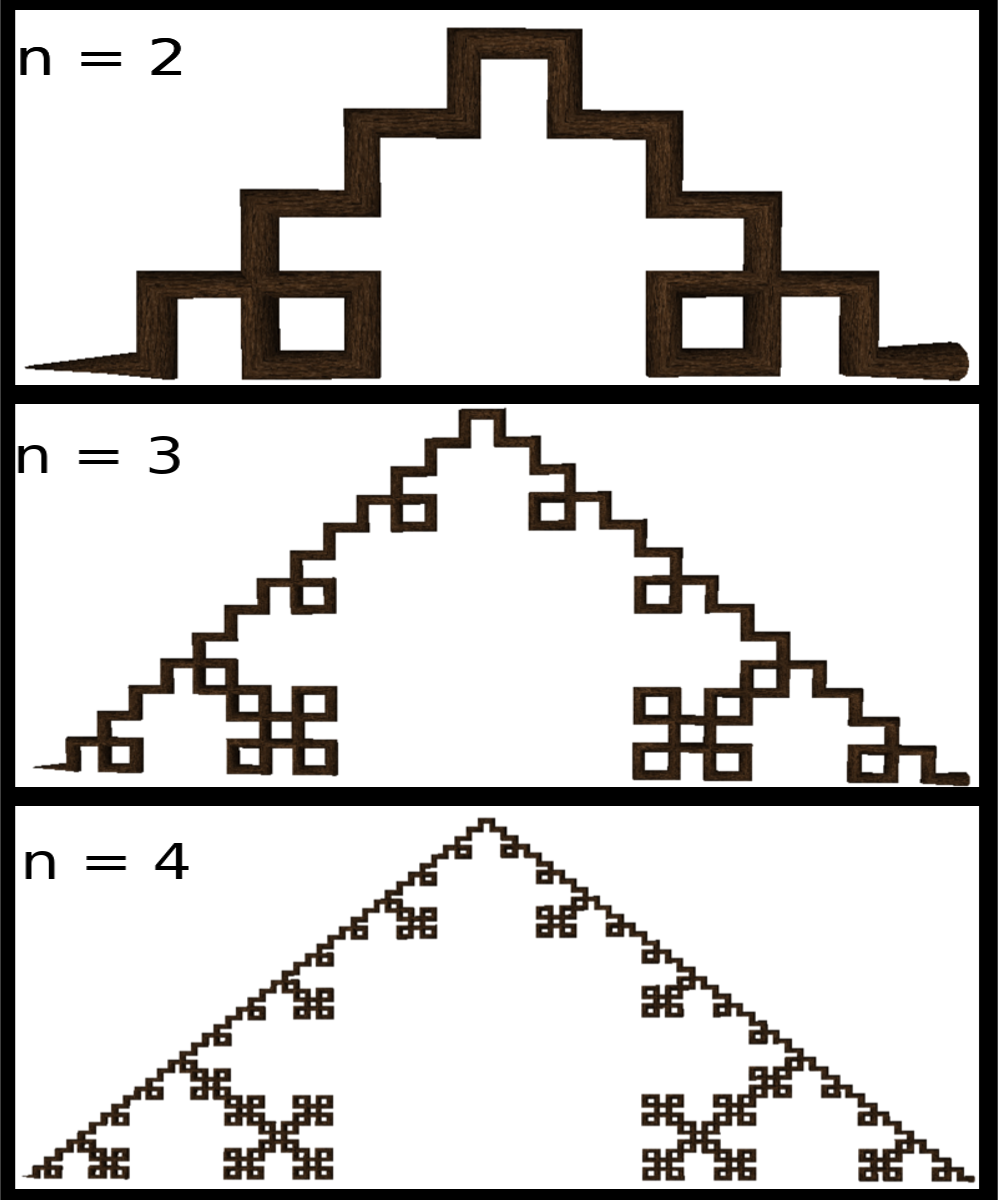
\includegraphics[scale=0.2]{Diagrams/koch_curves.png}
		\caption{Koch Curve.}
	}
\end{figure}
\begin{figure}[htbp]
	\raggedright
	\textbf{\underline{Sierpinski Triangles:}} \\
	Generations: 4\\
	Angle: 60$^\circ$\\
	Distance: 1 cm\\
	$\omega$ : F\\
	$p1$ : F $\rightarrow$ X-F-X\\
	$p2$ : X $\rightarrow$ F+X+F\\
	{\centering
		\vspace{7px}
		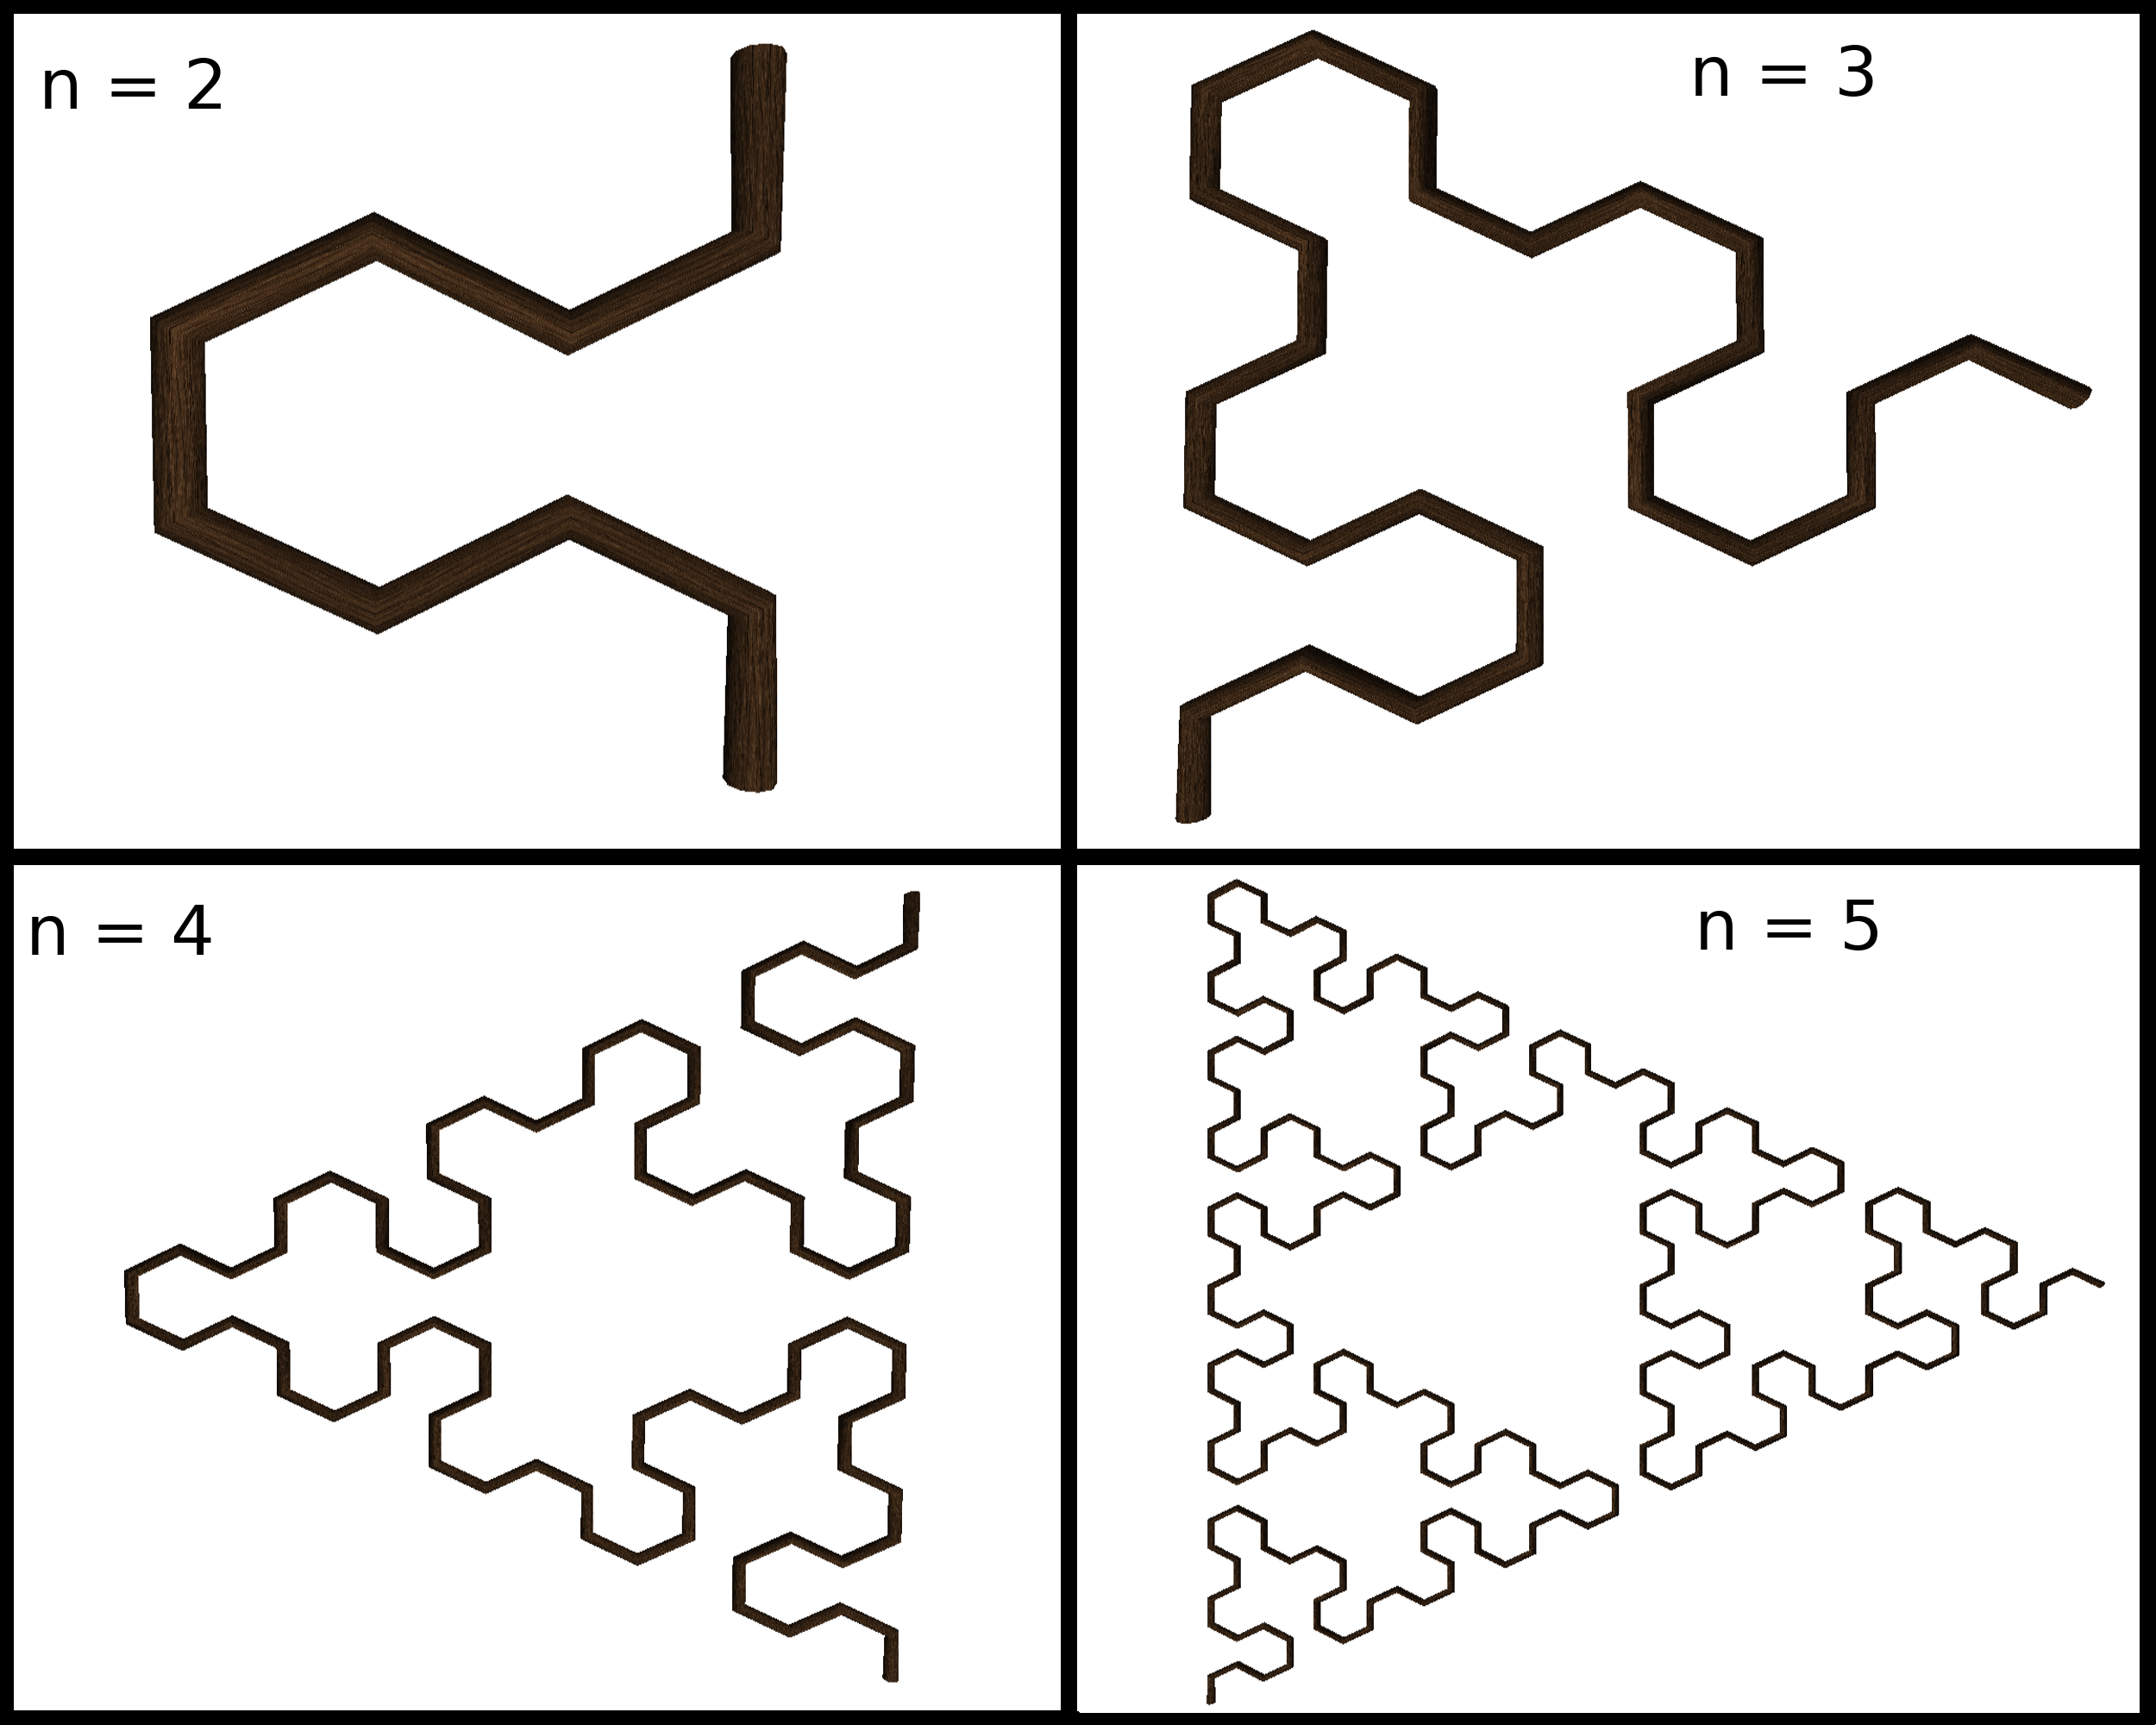
\includegraphics[scale=0.15]{Diagrams/sierpinsky_triangle.png}
		\caption{Sierpinski Triangles.}
	}
\end{figure}

\section{Branching} \label{branching}

The previous section covered a very basic 0L-system, which was capable of tracing a 3D pattern, the 0L-system allows us to move around a 3D space, however we are not able to branch off in two or more directions as plants do. Lindenmayer introduced two symbols which make branching much easier \cite{lindenmayer1968mathematical}. These are the square bracket commands '[', ']'. The square bracket characters instruct the turtle object to save its current position and orientation for the purpose of being able to go back to that saved position and orientation later. This allows the turtle to jump back to a previous position, facing the same direction as it was before. We can then change orientation and branch off in a different direction. This was originally used by Lindenmayer to develop the branching that occurs in algea, this idea was later used to represent plant-life by Smith \cite{smith1984plants}. 

The same method of interpreting the L-system string is applied, the symbols [ and ] are used in order the translate back to a previous position and orientation in order to branch off in a different direction. Each save state symbol [ must have a corresponding load state symbol within the string. In order to have a branch off of another branch we can have nested save and load state symbols. For instance the resultant string "F[+F-F]-F" branches off the main branch once as seen in figure \ref{branching 1}. Additionally using nested save and load states in the string "F[+F[+F]-F]-F" we are able to branch twice which can be shown in figure \ref{branching 2}.

\begin{figure}[htbp]
	{\centering
		\setlength{\fboxrule}{1pt}
		\vspace{7px}
		\fbox{
			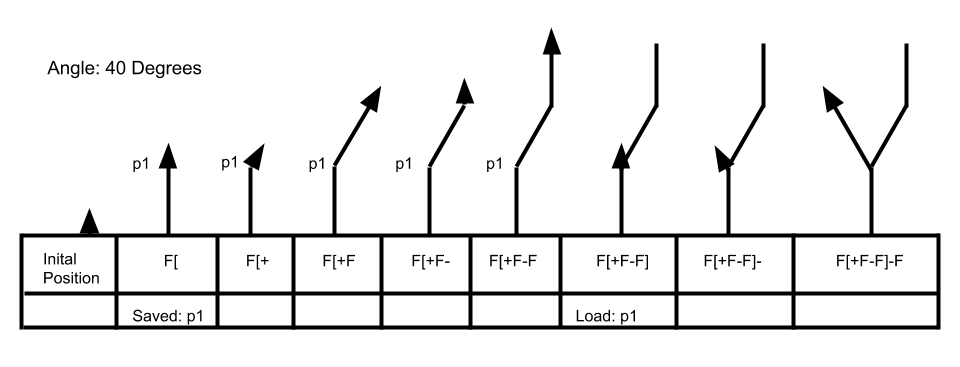
\includegraphics[scale=0.35]{Diagrams/branching.png}
		}
		\caption{Diagram showing a turtle interpreting an L-system using the branching symbols.} \label{branching 1}
	}
\end{figure}
\FloatBarrier

\noindent
Save and load operations are handled using the \acrfull{lifo} principle, meaning that when the save symbol is used [ the current position and orientation at $p1$ is saved, the next load state ] will restore $p1$'s position and orientation, unless another save takes place in which case that save will have to be loaded before $p1$ can be loaded. In this way, the position saves are stacked and the most recent save is loaded. This can be seen in figure \ref{branching 2} where we have nested branching. 

\begin{figure}[htbp]
	{\centering
		\setlength{\fboxrule}{1pt}
		\vspace{7px}
		\fbox{
			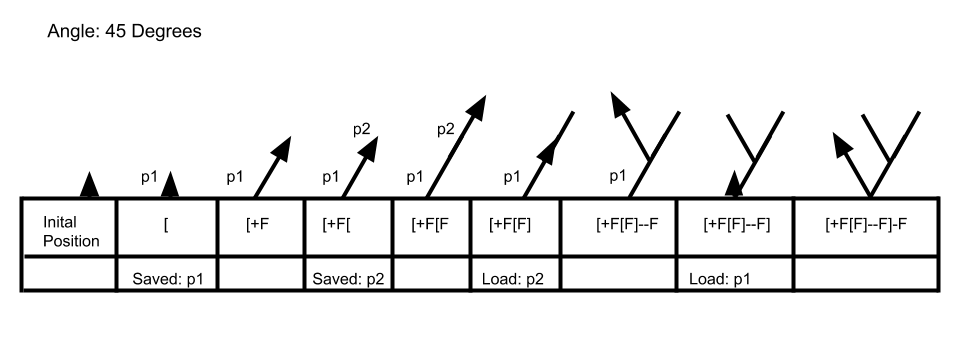
\includegraphics[scale=0.35]{Diagrams/NestedBranching.png}
		}
		\caption{Diagram showing a turtle interpreting an L-system with nested branching.} \label{branching 2}
	}
\end{figure}
\FloatBarrier

\noindent
The main advantage to using the save and load position functionality as a symbol within the alphabet of the L-system is that the rewiting system itself handles the branching. There is often no production rule for the save and load symbols and thus the symbols remain consistent from generation to generation. \\ 

\begin{figure}[htbp]
	\raggedright
	\textbf{\underline{Fractal Plant:}} \\
	\textbf{Alphabet:} X, F\\
	\textbf{Constants:} +, -, [, ] \\
	\textbf{Axiom:} X \\
	\textbf{Angle:} 25$^\circ$ \\
	\textbf{Rules:} \\
	X $\rightarrow$ F-[[X]+X]+F[+FX]-X\\
	F $\rightarrow$ FF \\
	{\centering
		\vspace{7px}
		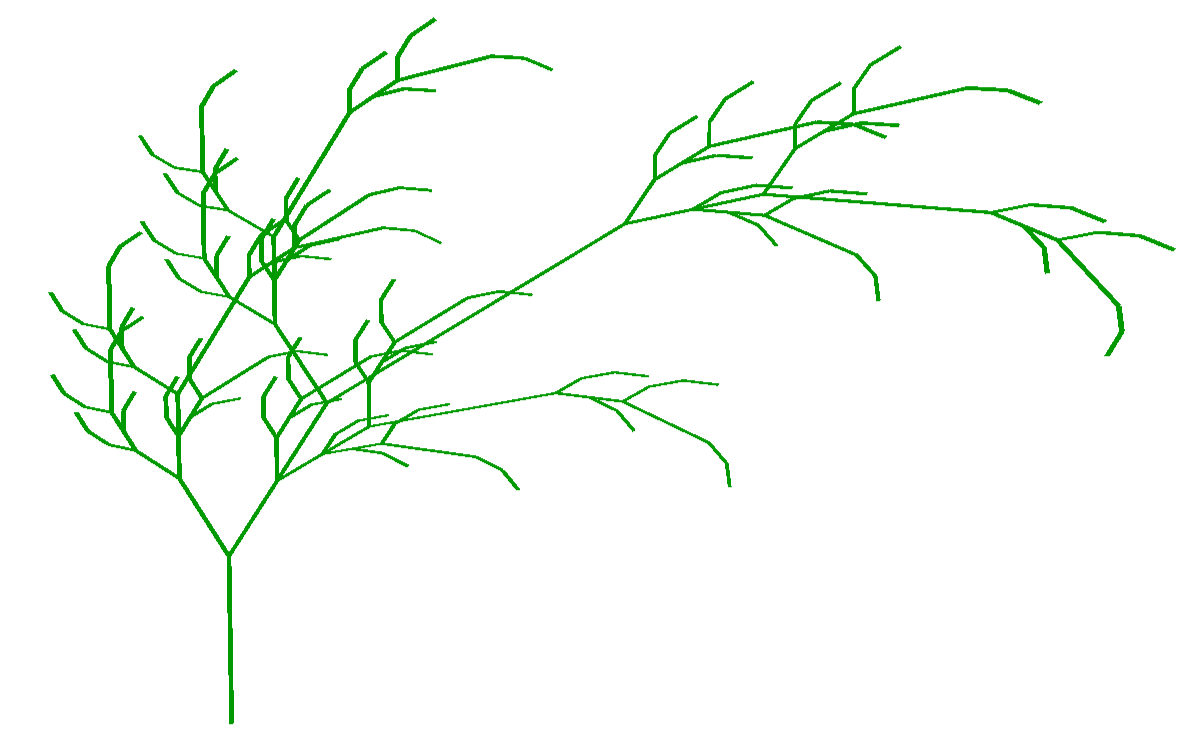
\includegraphics[scale=0.15]{FractalPlant/FractalPlant05.png}
		\caption{Fractal Plant.}
	}
\end{figure}
\FloatBarrier

\begin{figure}[htbp]
	\raggedright
	\textbf{\underline{Fractal Bush:}} \\
	\textbf{Alphabet:} F\\
	\textbf{Constants:} +, -, [, ] \\
	\textbf{Axiom:} F \\
	\textbf{Angle:} 25$^\circ$ \\
	\textbf{Rules:} \\
	F $\rightarrow$ FF+[+F-F-F]-[-F+F+F]\\
	{\centering
		\vspace{7px}
		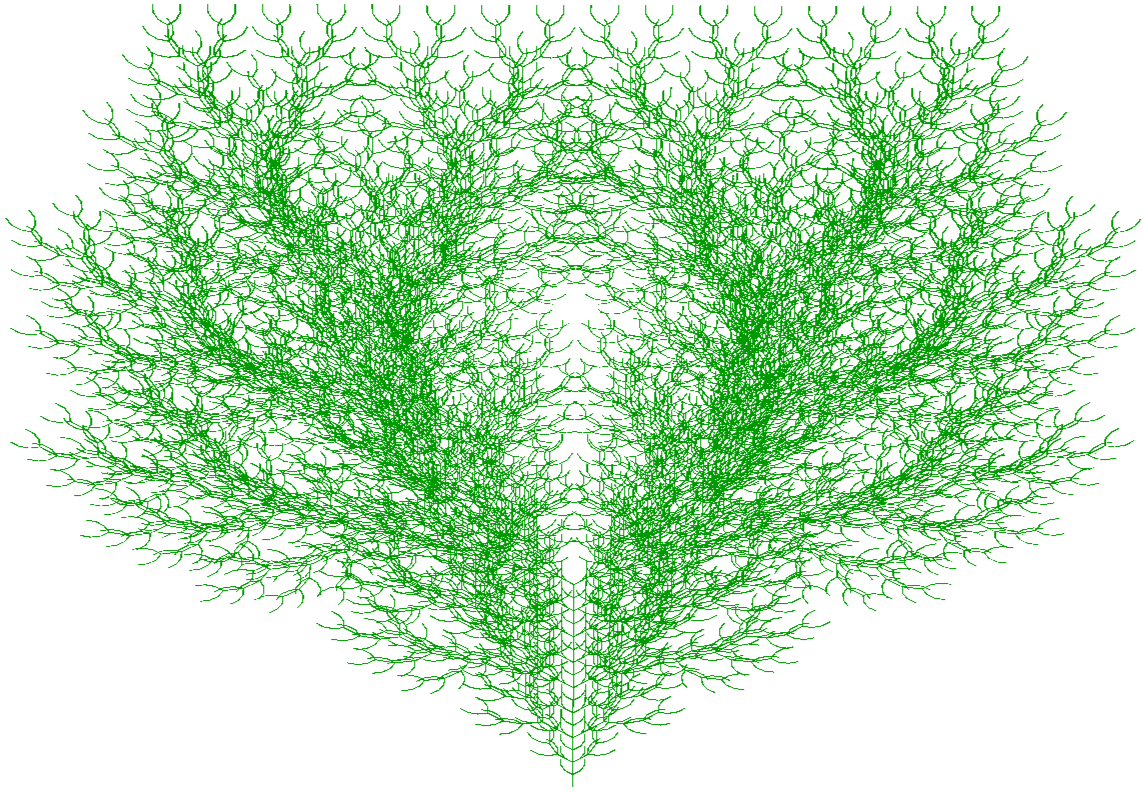
\includegraphics[scale=0.15]{FractalBush/FractalBush06.png}
		\caption{Fractal Bush.}
	}
\end{figure}
\FloatBarrier

\section{Parametric OL-systems} \label{parametric}

Simplistic L-systems like the algae representation in section \ref{Simple DOL-systems} above, give us enough information to create a very basic structure of plant life, there are many details that are not included which a simple OL-system will not be able to represent. With the simplistic approach we have assumed that the width and length and branching angles of each section is constant or predefined. The result of this was that all of the details such as width and length of branches is left up to the interpretation of the resultant L-system string. This begs the question as to how we should accurately interpret the L-system string when we are not provided the details by the L-system. The answer lies in parametric 0L-systems.

In this section I will outline the definition and major concepts of the parametric L-system formulated by Prusinkiewicz and Hanan in 1990 \cite{prusinkiewicz1990visualization}, and developed upon in 2012 by Prusinkiewicz and Lindenmayer \cite{prusinkiewicz2012algorithmic}. I will also be talking about some of the changes that I have made, and explaining why these changes are necessary for the purpose of this thesis.


\subsection{Formal Definition of a Parametric 0L-system} \label{definition of a parametric 0L-system section}

Prusinkiewicz and Hanan define the parametric 0L-systems as a system of parametric words, where a string of letters make up a module name $A$, each module has a number of parameters associated with it. The module names belong an alphabet $V$, therefore, $A~ \in~ V$, and the parameters belong to a set of real numbers $\Re$. If $(a_1,~ a_2,~ ...,~ a_n)~ \in~ R$ are parameters of $A$, the module can be stated as $A(a_1,~ a_2,~ ...,~ a_n)$. Each module is an element of the set of modules $M~ =~ V~ \times~ \Re^*$. $\Re^*$ represents the set of all finite sequences of parameters, including the case where there are no parameters. We can then infer that $M^*~ =~ (V~ \times~ \Re^*)^*$ where $M^*$ is the set of all finite modules. 

Each parameter of a given module corresponds to a formal definition of that parameter defined within the L-system productions. Let the formal definition of a parameter be $\Sigma$. $ E(\Sigma) $ can be said to be an arithmetic expression of a given parameter.\\ Similar to the arithmetic expressions in the programming languages C/C++, we can make use of the arithmetic operators $ +,~ -,~ *,~ \,~ \wedge{}$. Furthermore, we can have a relational expression $C(\Sigma)$, with a set of relational operators. In the literature by Prusinkiewicz and Hanan the set of relational operators is said to be $<,~ >,~ =$, I have extended this to include the relational operators $>,~ <,~ >=,~ <=,~ ==,~ !=$. Where $==$ is the 'equal to' operator and $!=$ is the 'not equal' operator, and the symbols $>=$ and $<=$ are 'greater than or equal to' and 'less than or equal to' respectively. The parentheses () are also used in order to specify precedence within an expression. A set of arithmetic expressions can be said to be $\hat{E} (\Sigma)$,  these arithmetic expressions can be evaluated and will result in the real number parameter $\Re $, and the relational expressions can be evaluated to either true or false. \\
\\
The parametric 0L-system can be shown as follows as per Prusinkiewicz and Hanan's definition:

\begin{equation}
G~ = (V, \Sigma, \omega, P)
\end{equation}
\vspace{5mm}

\noindent
$G$ is an ordererd quadruplet that describes the parametric OL-system. $V$ is the alphabet of characters for the system. $\Sigma$ is the set of formal parameters for the system. $\omega~ \in~ (V~ \times \Re^*)^+$ is a non-empty parametric word called the axiom. Finally $P$ is a finite set of production rules which can be fully defined as:

\begin{equation}
P~ \subset~ (V~ \times~ \Sigma^*)~ \times C(\Sigma)~ \times~ (V~ \times~ \hat{E}(\Sigma))^*
\end{equation}

\noindent
Where $(V~ \times~ \Sigma^*) $ is the predecessor module, $C(\Sigma) $ is the condition and $(V~ \times~ E(\Sigma))^* $ is the set of successor modules. For the sake of readability we can write out a production rule as \textit{predecessor} : \textit{condition} $\rightarrow$ \textit{successor}. I will be explaining the use of conditions in production rules in more detail in section \ref{Condition L-system Subsection}.
A module is said to match a production rule predecessor if they meet the three criteria below.

\begin{itemize}
\item The name of the axiom module matches the name of the production predecessor.
\item The number of parameters for the axiom module is the same as the number of parameters for the production predecessor.
\item The condition of the production evaluates to true. If there is no condition, then the result is true by default.
\end{itemize}

\noindent
In the case where the module does not match any of the production rule predecessors, the module is left unchanged, effectively rewriting itself. 


\subsection{Defining Constants and Objects}

There are some other features covered by Prusinkiewicz and Lindenmayer, that are not specific to the parametric L-systems definition itself but serve more as quality of life. In the literature, they refer to the \#define which is said "To assign values to numerical constants used in the L-system" as well as the \#include statement which specifies what type of shape to draw by refering to a library of predefined shapes \cite{prusinkiewicz2012algorithmic}.
\noindent
For instance if we have an value for an angle that we would like to use within the production rules we can use the \#define statement as follows:

\begin{equation} \label{define statement example}
\begin{aligned}
	&n=4 \\
	&\textrm{\#define angle 90}\\
	&\omega~~ : F(5)\\
	&p_1~ :  F(x)~~~~~ :~ * \rightarrow~ F(w)+(angle)F(w)+(angle)F(w)+(angle)F(w)\\
\end{aligned}
\end{equation}

Here you can see that the \#define acts like a declaration, where we are going to be defining a variable which will be used later. Essentially we are replacing any occurences of the variable \textit{angle} with the value of 90 degrees. The define statement is written as  \#define \textit{variable\_name} \textit{value}.

With regards to the \#include statement, In the literature the \#include may be used by stating \say{\#include H}. This would tell the turtle interpreter that the symbol \say{H} is a shape in a library of predefined shapes which should be rendered instead of the default shape. This functionality has been slightly modified, instead of the \#include statement, the \#object is used and serves a similar purpose, however, instead importing the symbol \say{H}, denoting to the hetrocist object from a library of predefined shapes, The statement \say{\#object H HETEROCYST} specifies that we are associating the symbol or module \say{H} with the object HETEROCYST. The HETEROCYST object is still stored in a predefined library, however, the advantage is that the object can be associated with multiple different symbols, it also does not limit us to a predefined name for an object. Below is an example using the \#object statement: 

\begin{equation} \label{object statement example}
\begin{aligned}
	&n=1 \\
	&\textrm{\#object F BRANCH}\\
	&\textrm{\#object S SPHERE}\\
	&\omega~~ : F(1)\\
	&p_1~ :  F(x)~~~~~ :~ * \rightarrow~ F(w)F(w)F(w)F(w)S(w)\\
\end{aligned}
\end{equation}

\begin{figure}[htbp]
	{\centering
		\vspace{7px}
		\setlength{\fboxrule}{1pt}
		\fbox{
			
\includegraphics[scale=0.2]{Diagrams/object_example.png}
		}
		\caption{Diagram of an L-system Using Multiple Objects.}
	}
\end{figure}
\FloatBarrier

\noindent
In the simple example in figure \ref{object statement example} above, you can see that the first three F modules render a branch segment with length of 1.0, however, for the final S module renders a sphere of diameter 1.0. The geometric shape that is eventually rendered does not affect the L-system in any way and the \#object feature bares no meaning to the rewriting system, it simply stands as an instruction to the interpreter which instructs that each time the symbols F or S are interpreted, a specific object should be rendered, such as BRANCH and SPHERE respectively. The position of the next object or branch can then be determined by moving forward by the diameter of the object and rendering the next object from that point, this will be discussed more detail chapter \ref{interpreter implementation} where the turtle graphics interpreter and renderer is defined.

\subsection{Modules With Special Meanings}

In the above section I defined the details of a parametric 0L-system, in the paper by Prusinkiewicz and Lindenmayer, there are two operators which I have not discussed yet, those are the ! and the ‘. Prusinkiewicz and Lindenmayer state that “The symbols ! and ‘ are used to decrement the diameter of segments and increment the current index to the color table respectively” \cite{prusinkiewicz2012algorithmic}. We have decided to modify this to work slightly differently, the ! and ‘ will still perform the same operation, however the ! and ‘ symbols are actually treated as a module that holds a particular meaning to the interpreter, rather than a single operator, furthermore, they share the same properties with modules, they can contain multiple parameters, and depending on the number of parameters they can be treated differently. The module ! with no parameters could mean decrement the diameter of the segment by a default amount, whereas !(10) means set the diameter of the segment to 10. The length can also be manipulated in a similar manner. The module with the name F has a default meaning to create a segment in the current direction by a default amount. If we provide the module F(10) we are specifying to create a segment of length 10.

Using the L-system below we can create figure \ref{parametric l-system practical}, the concepts discussed above have been used by decrementing the segment diameter during the rewriting process as well as by incrementing the branch length.

\begin{equation} \label{parametric l-system practical}
\begin{aligned}
	&n=8 \\
	&\omega~~ : A(5)\\
	&p_1~ :  A(w)~~~~~ :~ * \rightarrow~ F(1)!(w)[+A(w~*~0.707)][-A(w~*~0.707)]\\
	&p_2~ :  F(s)~~~~~ :~ * \rightarrow~ F(s~*~1.456)\\
\end{aligned}
\end{equation}

The above l-system gives the resulting representation shown below in figure 3.8. 

\begin{figure}[htbp]
	{\centering
		\vspace{7px}
		\setlength{\fboxrule}{1pt}
		\fbox{
			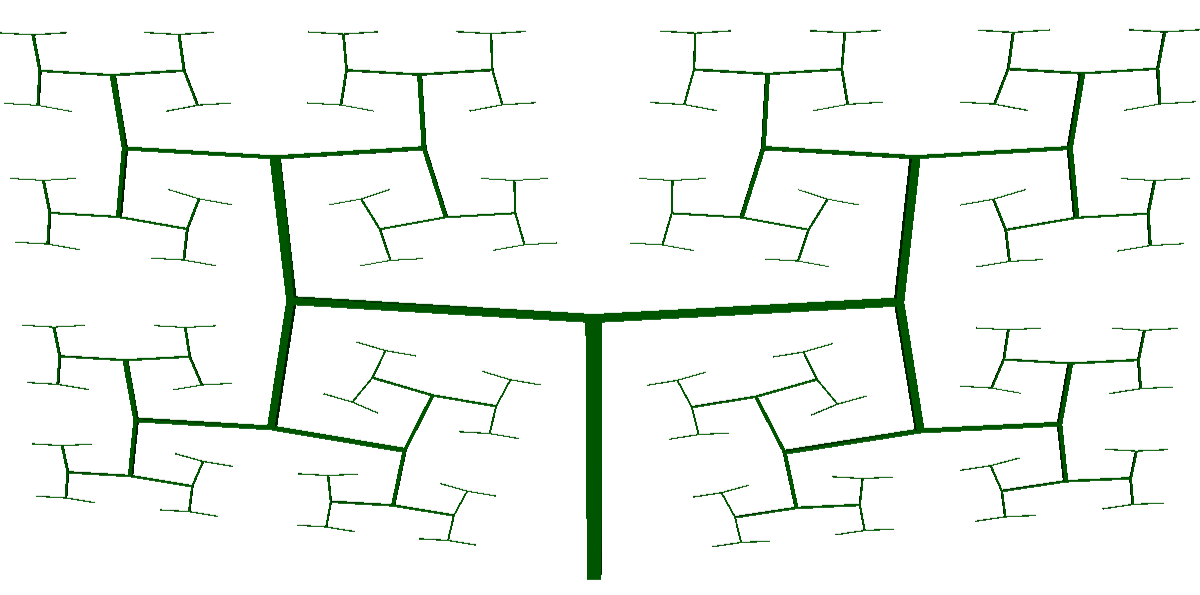
\includegraphics[scale=0.30]{ParametricLsystem/branchingPattern.png}
		}
		\caption{3D Parametric L-system.}
	}
\end{figure}
\FloatBarrier

\noindent
This gives a much more realistic looking tree structure as the branch segments become shorter but also become thinner in diameter as they get closer to the end of the branch as a whole. 

\subsection{Representing L-system Conditions} \label{Condition L-system Subsection}

A condition allows us to have multiple production rules that are the same in terms of the module name and the number of parameters that they have, furthermore, they require a particular condition to be met in order for the module to match that rule. 

In this section I will be detailing the use of the condition statement, which lies between the predecessor and the successor in a production rule, and can be seen as an a mathematical expression on either side of a relational operator. During the rule selection process the expressions are evaluated and the results are compared using the condition operator. If the result of the condition is true then that rule is selected for rewriting, if the result is false then it moves on to check the next rule. 


Below is an example of a parametric 0L-system using condition statements:

\begin{equation} \label{parametric l-system example}
\begin{aligned}
	&n=5 \\
	&\omega~~ : A(0)B(0,4)\\
	&p_1~ :  A(x)~~~~~ :~ x~ >~ 2~ \rightarrow~ C\\
	&p_2~ :  A(x)~~~~~ :~ x~ <~ 2~ \rightarrow~ A(x~ +~ 1)\\
	&p_3~ :  B(x,~ y)~ :~ x~ >~ y~ \rightarrow~ D\\
	&p_4~ :  B(x,~ y)~ :~ x~ <~ y~ \rightarrow~ B(x~ +~ 1,~ y)\\
\end{aligned}
\end{equation}

\noindent
The L-system above in \ref{parametric l-system example} is rewritten five times using the axiom specified by the symbol $\omega$, as well as the four production rules $p_1, p_2, p_3, p_4$. Each generation of the rewritting process can be seen below in \ref{parametric l-system example result}.

\begin{equation} \label{parametric l-system example result}
\begin{aligned}
	&g_0 :~ A(0)B(0,~4)\\
	&g_1 :~ A(1)B(1,~4)\\
	&g_2 :~ A(2)B(2,~4)\\
	&g_3 :~ C~B(3,~4)\\
	&g_4 :~ C~B(4,~4)\\
	&g_5 :~ C~D\\
\end{aligned}
\end{equation}

\noindent
A practical use of the condition statement might be to simulate different stages of growth. This is best illustrated using the L-system below: 

\begin{equation} \label{conditional l-system example}
\begin{aligned}
	&n=2,~4,~6 \\
	&\#\text{object F BRANCH} \\
 	&\#\text{object L LEAF} \\
	&\#\text{object S SPHERE} \\
	&\#\text{define r 45} \\
	&\#\text{define len 0.5} \\
	&\#\text{define lean 5.0} \\
	&\#\text{define flowerW 1.0} \\
	&\omega~~ :~ !(0.1)I(5)\\
	&p_1~ :  I(x)~ :~ x~ >~ 0~~ \rightarrow~ F(len)-(lean)[R({0, 100})]F(len)[R({0, 100})]I(x-1)\\
	&p_2~ :  R(x)~ :~ x~ >~ 50~ \rightarrow~ -(r)/(20)!(2.0)L(2)!(0.1)\\
	&p_3~ :  R(x)~ :~ x~ <~ 50~ \rightarrow~ -(r)\backslash(170)!(2.0)L(2)!(0.1)\\
	&p_4~ :  I(x)~ :~ x~ <=~ 0~ \rightarrow~ F(len)!(flowerW)S(0.3)\\
\end{aligned}
\end{equation}

\begin{figure}[htbp]
	{\centering
		\vspace{7px}
		\setlength{\fboxrule}{1pt}
		\fbox{
			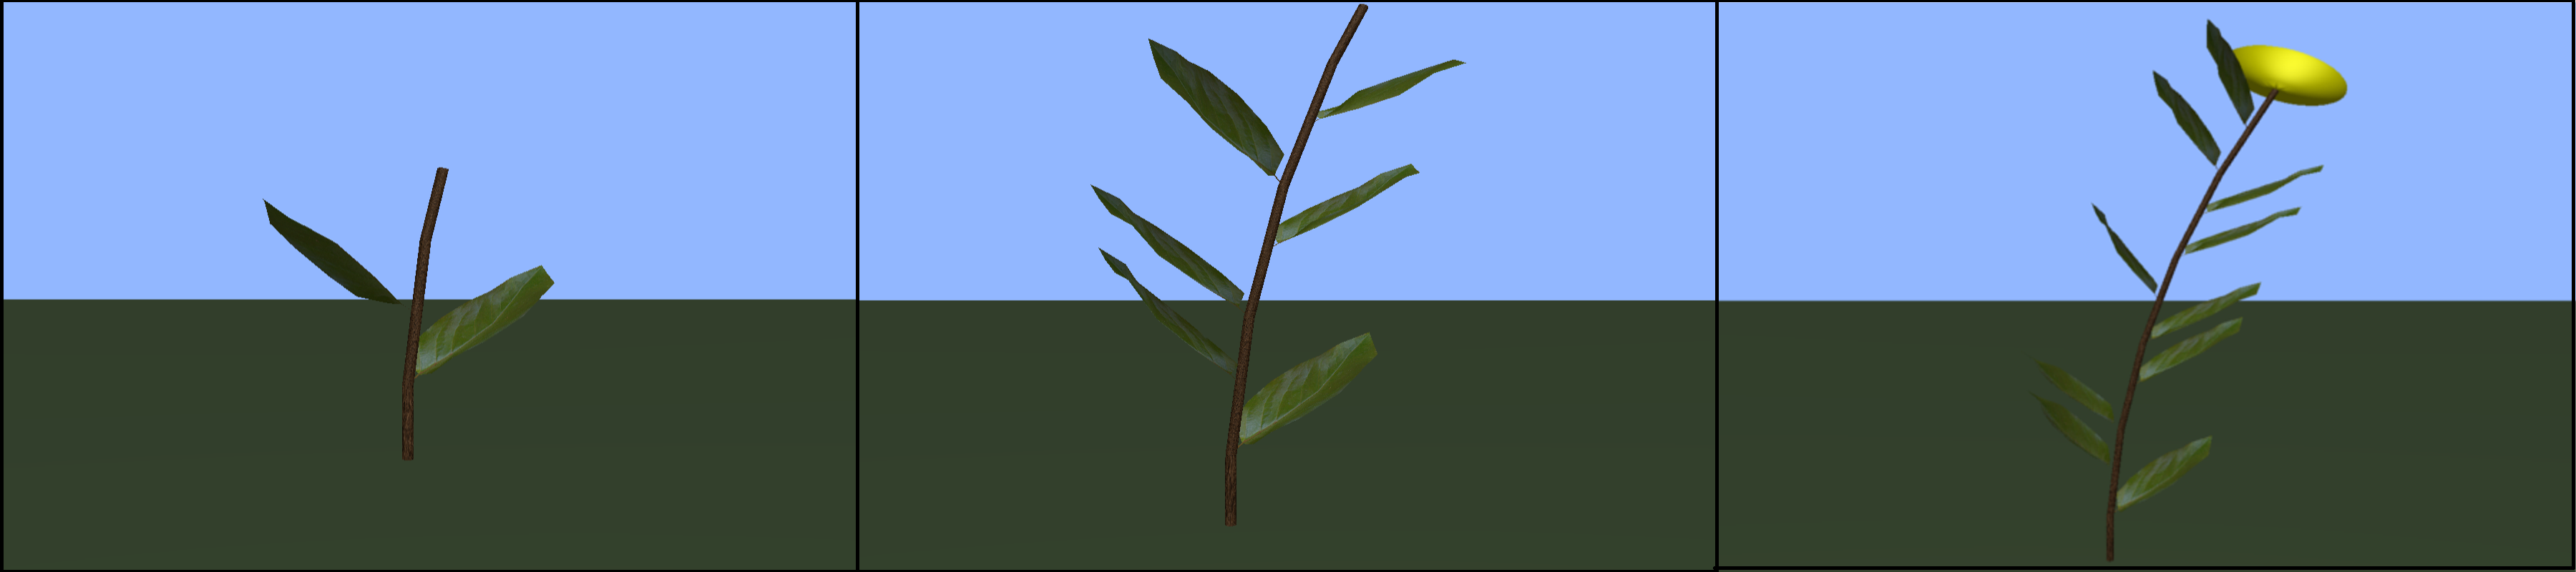
\includegraphics[scale=0.12]{Diagrams/conditionalLsystem.png}
		}
		\caption{Condition statements used to simulate the growth of a flower. 2nd generation on the left, 4th generation in the center and 6th generation on the right}
	}
\end{figure}
\FloatBarrier


\section{Randomness within L-systems} \label{Randomness L-system Subsection}

Randomness is an essential part of nature. If there was no randomness in plant life, it would end up with very symetric and unrealistic. Randomness is also responsible for creating variation in the same L-system. A L-system essentially describes the structure and species of a plant. It describes everything from how large the trunk of the tree is, to how many leaves there are on the end of branch, or even if it has flowers or not. However if there is no capability to have randomness in the generation of the L-system then we will always end up with the exact same structure. 
\vspace{5mm}
Below is a simple example of how randomness can be used to create variation.

\begin{equation} \label{randomness example}
\begin{aligned}
	&n=2\\
	&\text{\#define r 25} \\
	&\omega~~ :~ !(0.2)F(1.0)\\
	&p_1~ :  F(x)~ :~ *~ \rightarrow~ F(x)[+(r)F(x)][-(r)F(x)]+(\{-20, 20\})F(x)-(\{-20, 20\})F(x)\\
\end{aligned}
\end{equation}

\begin{figure}[htbp]

	{\centering
		\setlength{\fboxrule}{0pt}
		\fbox{
			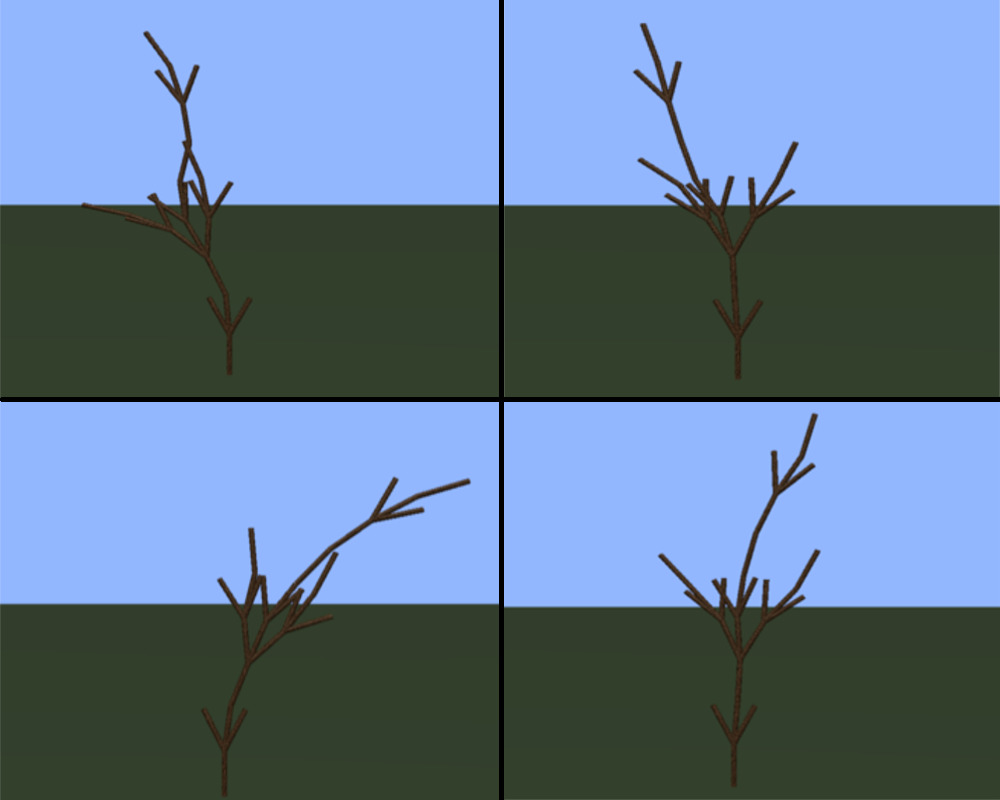
\includegraphics[scale=0.15]{Diagrams/RandomTrees.png}
		}
		\caption{Different Variations of the Same L-system with Randomness Introduced in The Angles. \label{figRandomness}}
	}
\end{figure}
\FloatBarrier

\noindent
In figure \ref{figRandomness} there are four variations of the same L-system using randomness, We can specify that we would like to create a random number by using the expression \{-20.0, 20.0\}. The curly braces signify that what is contained is a random number range, ranging from the minimum value as the first floating point value and the maximum value as the second floating point value separated by a comma. If both values are the same for instance +(\{10.0, 10.0\}) this is equivilant to +(10.0).

\section{Stochastic Rules within L-systems} \label{Stochastic L-system Subsection}

Similar to the previous section about randomness in L-systems, stochastic L-systems fulfill a similar goal. 0L-systems on their own are incapable of creating any variation, they simply follow a strict set of production rules which gives the same result. Introducing randomness to an 0L-system for width, length and other parameters can result in a plant that looks slightly different but does not change to overall structure of the plant or any branching. In order to create a different structure for a plant we must introduce stochastic probability within the selection of the production rules, thus effecting the rewriting of the structure itself.

Eichhorst and Savitch introduced a new type of 0L-system called the S0L-system, this added two features to the existing 0L-system, firstly the S0L-system is not limited to defining a single axiom (starting point), a finite number of starting points can be defined and a probability distribution is used in order to select the starting point at the start of the rewriting process. Secondly, the S0L-system allows you to define a finite number of production rules which have a probability distribution in order to decide which rule should be chosen for rewriting \cite{eichhorst1980growth}. Similarly an article by Yokomori proposes a stochastic 0L-system which also proposes a measure of the entropy of a string generated by a 0L-system \cite{yokomori1980stochastic}.\\
Later, Prusinkiewicz and Lindenmayer built upon this by creating a definition of a stochastic L-system, that makes use of the stochastic nature of the production rules from the SOL-system. In this paper, I will be using the definition of the stochastic 0L-system defined by Prusinkiewicz and Lindenmayer, and developing them into the existing parametric 0L-system. This paper will not allow multiple starting points as defined by Eichhorst and Savitch in the SOL-system, as it does not seem necessary and could overcomplicate the 0L-system, however, this functionality could be added in the future if it is seen to be neccessary. \\
Similarly to the 0L-sysstem, the stochastic 0L-system is an ordered quadruplet, represented as $G_\pi~ = (V, \omega, P, \pi)$, where $V$ is the alphabet of the 0L-system, $\omega$ is the axiom, $P$ is the finite set of productions and $\pi$ represents a probability distribution for a set of production probabilities this can be shown as $\pi~ :~ P~ \rightarrow~ (0, 1)$ the production probabilities must be between 0 and 1 and the sum of all production probabilies must add up to 1.

The following L-system definition created by Prusinkiewicz and Lindenmayer states three production rules with each rule having a probability of 0.33 out of one. For a finite set of production rules to be stochastic, the production rules must share the same module name an the same number of parameters. There must be two or more production rules and the total probability distribution must add up to 1.0 \cite{prusinkiewicz2012algorithmic}.

\begin{equation} \label{stochastic example}
\begin{aligned}
	&n=5\\
	&\text{\#define r 25}\\
	&\omega~~ :~ F(1)\\
	&p_1~ :  F(x)~ :~ \sim 0.33 ~ \rightarrow~ F(x)[+(r)F(x)]F(x)[-(r)F(x)]F(x)\\
	&p_2~ :  F(x)~ :~ \sim 0.33 ~ \rightarrow~ F(x)[+(r)F(x)]F(x)\\
	&p_3~ :  F(x)~ :~ \sim 0.34 ~ \rightarrow~ F(x)[-(r)F(x)]F(x)\\
\end{aligned}
\end{equation}

\noindent
As you can see the module F(x) above, is the predecessor for all three of the production rules, each rule has a probability which is defined using the $\sim$ symbol followed by probability from 0 to  1. In the above example each probability isapproximately one third, they are approximate in order to total a an exact probability of 1.0. During the rewriting process, when the module F with one parameter is found, a production rule is randomly selected using the probability distribution described within the production rule. The predecessor from the selected rule with then rewrite that module. 

\begin{figure}[htbp]
	{\centering
		\vspace{7px}
		\setlength{\fboxrule}{1pt}
		\fbox{
			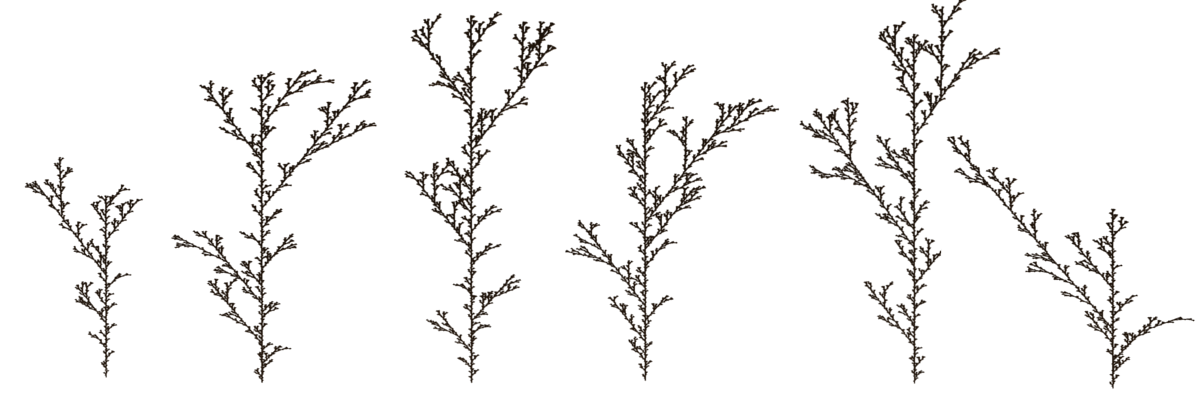
\includegraphics[scale=0.35]{Diagrams/stochastics.png}
		}
		\caption{Representation of an L-system with a probability stochastic with a 0.33 probabability for each rule.} \label{stochastic diagram}
	}
\end{figure}
\FloatBarrier

\noindent
The stochastic L-system definition in \ref{stochastic example}, produces the following fractal structures seen in figure \ref{stochastic diagram} below. The stochastic L-system will get a slightly different resultant string each time it is run, depending on which rules were selected for rewriting. This gives a different number of translation instructions, can result in the plants having branches of different lengths, for example $p1$ has two extra F instructions. Resulting in some branches being much longer than others, as well as possibly producing plants of different sizes. 

\begin{figure}[htbp]
	{\centering
		\setlength{\fboxrule}{1pt}
		\vspace{7px}
		\fbox{
			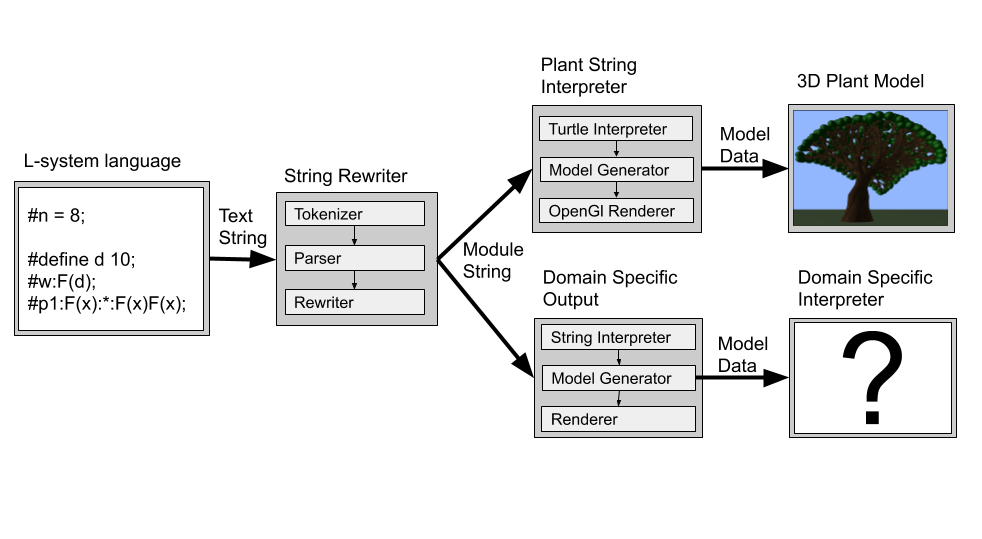
\includegraphics[scale=0.43]{Diagrams/FullDiagram.png}
			\label{3DAxisFigure}
		}
		\caption{Diagram of the procedural generation process.}
	}
\end{figure}
\FloatBarrier

\section{Summary}

L-systems represent a set of state transitions based upon the production rules provided, these rules dictate how a string will be rewritten, which in turn determines the overall structure of the plant it is trying to represent. The symbols in D0L-systems or modules in parametric 0L-systems represent particular instructions to be carried out by turtle graphics within the interpreter. The symbols or modules within an L-system do not change the behaviour of the L-system but matter only to the interpreter. Additionally the complexity of the L-system rewriter decides the complexity of the interpreter, if a L-system provides a large amount of information to the interpreter, less assumptions need to be made during the interpretation and therefore, providing the able to more accurately describe the plant-life it is representing.

By using the parametric 0L-system we can build in a number of features, otherwise used in other L-systems, such as branching, conditional production rules, randomness in parameters, stochasticity. These features allow the parametric 0L-system to represent plant-life with varying structures as well as branch lengths, branch widths and production rule conditions can give control over stages of growth.



\chapter{L-system Rewriter Implementation}

\lettrine[lines=3]{T}{}here are two major parts necessary to procedurally generate plant-life using an L-system. These are the rewriter and the interpreter. The purpose of the L-system rewriter is to take an L-system file as input, and generate the resulting string that fits the L-system grammar. It does this by syntactically and semantically analysing the L-system input, and generating the structures and information necessary to carry out the rewriting process. The rewriting process uses the structures and information, such as the string of modules and the production rules, to step through each string and rewrite the symbols. This chapter focuses on each part of the string rewriters' implementation and will introduce a technique of processing the L-systems' input, similar to how computer languages are compiled. This chapter will also formally define the L-system grammar in Backus-Naur Form, and provide the pseudocode for the L-system rewriter. 

For a simple D0L-system, like the one seen in section \ref{DOL-system example}. Each symbol within the alphabet is made up of a single character, the productions rules then match against those characters. As the D0L-system is deterministic, there is no randomness when determining the matching rule. The simplicity of the L-system makes it quite easy to create a rewriting system for the D0L-system. All the rewriter must do is store the starting string and production rule predecessors and successors. It then iterates over a string of symbols and replace them with the successor. The implementation of a more sophisticated L-system, like the parametric 0L-system, is much more complex. A parametric L-system can have multiple modules that make up a string, where each module may have multiple parameters, and each parameter could be a mathematical expression. The added complexity makes developing a rewriting system considerably more difficult. The rewriter must better understand what the syntax of the L-system is specifying, based on the context of each symbol within the L-system.

Due to the complexity of the L-system grammar, it is difficult for a computer to tell the syntactic and semantic properties of each part of the L-system input, which makes it difficult to carry out the rewriting process. Using a system similar to a \say{compiler}, an L-system "program" can be broken down into a three-stage process, as seen in figure \ref{3D rotations} below. The first stage is \textit{lexical analysis}, then a process called \textit{parsing} and finally the string rewriting stage. The lexical analyser is responsible for splitting the input into syntactic words, and then assigning each word into its syntactic category. Any word within the L-system that does match a syntactic category will result in a lexical error. If there are no lexical errors the words and their syntactic categories are sent to the parser. The parser matches the syntactical categories of each sentence in the language against a grammatical model. If any of the sentences within the language do not match the grammatical model, an appropriate error message can be displayed, similar to that of the lexical error. The error states where the syntax error occurred and what was grammatically incorrect. The parser also creates a syntax tree along with any data structures necessary for the rewriting process. These structures can then be used to carry out string rewriting or provide information to the interpreter.

\begin{figure}[htbp]
	{\centering
		\setlength{\fboxrule}{1pt}
		\vspace{7px}
		\fbox{
			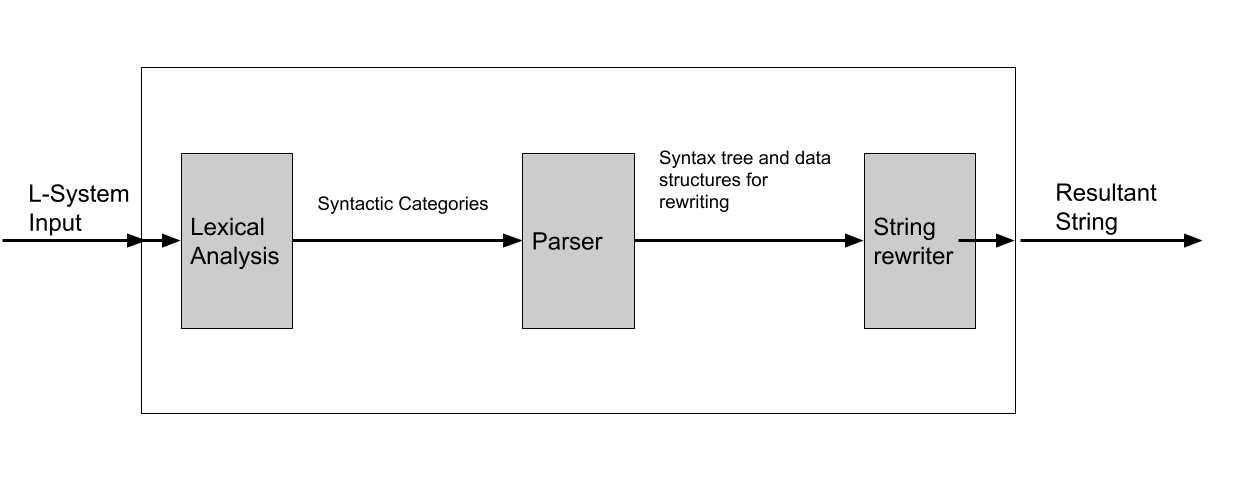
\includegraphics[scale=0.32]{Diagrams/StringRewriter.png}
		}
		\caption{Diagram of the Parts of The Rewiting System.} \label{3D rotations}
	}
\end{figure}
\FloatBarrier

\section{Environment and Tools}

The implementation of the string rewriter, and the string interpreter, is written in the C and C++ programming languages \cite{stroustrup2000c++}. The C and C++ languages are two of the most common programming languages that have stood the test of time with the first version of C being released in 1974. These languages are frequently used within computer graphics, with some of the most popular game engines supporting either C or C++. Such as CryEngine, Unreal Engine, Source Engine, and more. The main reason for this is the high performance and low-level memory management that C and C++ provide, and the graphics programming frameworks such as OpenGL, Vulkan, and DirectX all having direct support for either C or C++. The C and C++ languages also have a large number of useful libraries that provide extra functionality.  

The implementation of the rewriter and the interpreter will use the modern Open Graphics Library (\gls{OpenGL}). The OpenGL framework is one of the industry standards for creating 3D graphics applications. It is a cross-platform API for interacting with the \acrshort{gpu} in a low-level way. The high-performance nature of OpenGL is essential, as displaying and simulating the L-system can be very graphically intensive \cite{sellers2013opengl} \cite{movania2017opengl}. OpenGL was initially intended to be an \acrshort{api} for the C and C++ programming languages. Therefore, both the programming language and graphics API have a strong emphasis on performance, which is necessary when procedurally generating and simulating plant-life.

For more specialised mathematics capabilities, the \acrfull{glm} library holds many mathematics classes and functions for conveniently dealing with structures such as vectors, matrices, and quaternions. This thesis will cover these mathematical concepts in chapter \label{maths chapter}; however, it is convenient to have these implemented and tested within a C++ library. Another important library is \acrfull{glfw} which is a multi-platform \acrshort{api} for creating an managing user interface windows, events, and user-input \cite{glfwDocumentation}. To keep track of changes and manage versions. Git is a free and open-source version control software. It can keep track of changes that have been made to the files within a project folder as well as keep previous versions of the project throughout the development process. In conjunction with Git,  Github is an online web application that stores git repositories. Git acts as a backup as well as containing all previous versions of the project \cite{torvalds}.

\section{The L-system as an Interpreted Grammar}

Traditionally an interpreter in computing is a program that takes program code as input. It is then analyzed and interpreted as it is encountered in the execution process. All of the previously encountered information is kept for later interpretations. The information about the program can be extracted by inspecting the program, such as the set of declared variables in a block or a function \cite{wilhelm2010compiler}. In essence, the L-system rewriter contains a type of interpreter. This should not be confused with the interpreter that processes the resultant string using turtle graphics. Due to this confusion of terms, the system containing the lexical analyser, L-system parser, and the string rewriter will be referred to as the L-system rewriter, instead of the interpreter in the computational sense. 

A similarity can be drawn between traditionally interpreted languages and the L-system rewriter. The L-system rewriter defines a set of constant variables, a starting point, and then some production rules. This information can then be used to rewrite the starting string several times. Later on, it may be decided that, instead of five generations of rewriting, the rewriter should instead generate ten. Some information about the L-system is still valid, the production rules, axiom, and constants have not changed, and therefore this information can be used to interpret to the tenth generation. This concept can be used to go from the current state of the L-system rewriter and rewrite another five times. Instead of throwing all the information away and starting from scratch. Furthermore, if we would like to retrieve the resultant string, this can be requested from the L-system rewriter. 

The lexical analyser and parser are a necessary part to carry out rewriting. Without the lexical analyser or parser, it would not be straightforward to find the syntactic roles of each part of the L-system. Take the example of the module: F(2*3, x * (2 + y)). Here there is a single module with two parameters, one parameter has the expression (2 * 3), and the other has the expression (x * (2+y)). These complex structures within a grammar require knowledge about the grammatical model it represents. The lexical analyser firstly makes sure that all the syntax within the L-system is correct and assigns each word or symbol to a syntactic category, the parser then splits the L-system into its components and is describes each parts syntactic roll. The lexical analyser provides the understanding that x and y are variables within a module and do not represent something else. It also provides knowledge about how to find the values of x and y. 

The difficulty of creating an L-system with more complexity in the grammar is that it becomes more challenging to write a valid L-system to represent a particular structure. For example, imagine trying to write a C program where the compiler does specify why the program is incorrect. The advantage of using a rewriter similar to a compiler is that it makes it simpler to debug any syntactic errors, as well as make the string rewriting much faster. This means that writing an L-system becomes similar to rewriting a recursive program, where any syntactic mistakes will result in a meaningful error describing what was incorrect.

\section{The Syntax of a Parametric L-system}

This section will specify the valid syntax for the parametric L-system rewriter. The syntax is similar to the definition of the parametric L-system definition given by Prusinkiewicz and Lindenmayer in section \ref{definition of a parametric 0L-system section}. There are some additions and modifications to the syntax definition provided by Prusinkiewicz and Lindenmayer to construct an L-system that includes branching, constant variable definitions, object specifications, parametric L-system concepts, randomness, and stochastic L-systems \cite{prusinkiewicz2012algorithmic}. 

This L-system has five major parts. Each part is categorised as a statement. Valid statements are the \textit{defines} , the \textit{includes}, a single generation statement, a single axiom statement, and one or more production rules \cite{prusinkiewicz2013lindenmayer}. All of these statements collectively form an L-system. Each statement starts with a `\#' character and ends with a `;' symbol. These are used to indicate the start and end of a statement, even if multiple statements are written on the same line. 

The order that statements should be listed is as follows: 

\begin{equation} \label{statement order example}
\begin{aligned}
	&\text{\#generations statement;}\\
	&\text{\#define statements;}\\
	&\text{\hspace{10mm}...}\\
	&\text{\#include statements;}\\
	&\text{\hspace{10mm}...}\\
	&\text{\#axiom statement;}\\
	&\text{\#production statements;}\\
	&\text{\hspace{10mm}...}\\
\end{aligned}
\end{equation}

The order for the statements does not always matter; for instance, the generation statement can be defined anywhere within the L-system. However, some parts are required to be in a particular order, such as the define and include statements, which must appear above the axiom and production rule statements as they define values used within the axiom and production rules. It is best practice to specify the L-system in the above order as to avoid any conflictions or errors.

All numbers within the L-system are represented as floating-point numbers. Using a single data-type keeps all numbers consistent. Other data types could be added in the future; however, there are added complexities in doing so, such as the conversion from one type to another, or having to specify which data type a variable represents. The floating-point data type provides all the necessary functionality needed for the L-system; therefore, it seems unnecessary to add more data types. 

\section{The L-system Lexical Analyser} \label{Flex}

In computer science, specifically the study of programming language compilers, the program responsible for carrying out lexical analysis is the lexer. Depending on the literature the lexer can also be known as the tokenizer or scanner. D. Cooper and L. Torczon write that ``The scanner, or lexical analyser, reads a stream of characters and produces a stream of words. It aggregates characters to form words and applies a set of rules to determine whether each word is legal in the source language. If the word is valid, the scanner assigns it a syntactic category or part of speech'' \cite{cooper2011engineering}. This is no different for the parametric 0L-system rewriter. For the rewriter to have enough information to carry out rewriting, it must first understand what each word or token within the L-system means, this requires assigning a syntactic category to each token, and whether or not the token is valid or not within the L-system grammar.  

The scanner itself is quite complex, its main goal is to match the characters or strings within the language, to either a word or a regular expression defined in the grammar. When the match is made the token is given a syntactic category. The mechanism by which it achieves this is known as \textit{finite automata} \cite{wilhelm2013compiler}. It is possible to write custom \gls{Lexer}, however, it can be quite complicated and time-consuming to design and implement, and once a custom \gls{Lexer} has been created it is also difficult to change functionality at a later stage. There is a well known program known as the \acrlong{flex} (\acrshort{flex}). \acrshort{flex} takes in a file which contains the lexical rules of the language, this being the strings as well as the regular expression as well as its associated syntactic category. When \acrshort{flex} is executed it will create a \gls{Lexer} in the form of a C program. To create a lexer with \acrshort{flex}, the lexical rules must be defined. Below are the characters, strings and regular expressions and their associated syntactic categories, as well as a description as to its use in the parametric 0L-system. 

\begin{table}[h!] \center
\begin{tabular}{ | c | l | l |}
\hline
	Syntactic Word	& Syntactic Category & Description\\  
\hline
\hline
	, 				& T\_COMMA 				& Separation between module parameters \\
\hline
	: 				& T\_COLON 				& Separation between production rule parts \\
\hline
	; 				& T\_SEMI\_COLON 		& End of a statement\\
\hline
	\#				& T\_HASH 				& Beginning of a statement\\
\hline
	( 				& T\_PARENL 			& Start of a modules parameters \\
					&						& or specifies presidence in an expression \\
\hline
	) 				& T\_PARENR 			& End of a modules parameters \\
					&						& or specifies presidence in an expression \\
\hline
	\{ 				& T\_BRACKETL 			& Start of a random range\\
\hline
	\} 				& T\_BRACKETR 			& End of a random range\\
\hline
	$\sim$ 			& T\_TILDE 				& Stochastic operator\\
\hline
	$==$				& T\_EQUAL\_TO 			& Relational operator stating equal to\\
\hline
	$!=$				& T\_NOT\_EQUAL\_TO 	& Relational operator for not equal to\\
\hline	
	$<$ 			& T\_LESS\_THAN 		& Relational operator for less than\\
\hline
	$>$ 			& T\_GREATER\_THAN 		& Relational operator for greater than\\
\hline
	$<=$ 			& T\_LESS\_EQUAL 		& Relational operator for greater or equal\\
\hline
	$>=$  			& T\_GREATER\_EQUAL 	& Relational operator for greater or equal\\
\hline
	[ 				& T\_SQUARE\_BRACEL 	& Module name (branching save state) \\
\hline
	] 				& T\_SQUARE\_BRACER 	& Module name (branching load state) \\
\hline
	+ 				& T\_PLUS 				& Arithmetic operator for addition, or\\
					&						& Module name (Yaw right) \\
\hline
	- 				& T\_MINUS 				& Arithmetic operator for subtraction, or\\
					&						& Module name (Yaw left)\\
\hline
	/ 				& T\_FORWARD\_SLASH 	& Arithmetic operator for division, or\\
					&						& Module name (Pitch up)\\
\hline
	$\backslash$ 		& T\_BACK\_SLASH 		& Module name (Pitch down)\\
\hline
	* 				& T\_STAR 				& Arithmetic operator for multiplication, or\\
					&						& Condition in a production rule which is true\\
\hline
	$\land$		& T\_HAT 				& Arithmetic operator for and exponent, or\\
					&						& Module name (Roll right)\\
\hline
	$\&$ 			& T\_AMPERSAND 			& Module name (Roll left)\\
\hline
	! 				& T\_EXCLAMATION 		& Module name (Set size of branch)\\
\hline
	\$ 				& T\_DOLLAR 			& Module name \\
\hline
	= 				& T\_ASSIGN 			& Assignment operator used to set generations\\
\hline
	\#n 			& T\_GENERATIONS 		& Declaration of the number of generations\\
\hline
	\#w 			& T\_AXIOM 				& Declaration of the axiom\\
\hline
	\#define 			& T\_DEFINE 		& Declaration of the define\\
\hline
	\#object 			& T\_OBJECT			& Declaration of the object\\
\hline
	[0-9]+.[0-9]+$|$[0-9]+ 					& T\_FLOAT 				& Regular expression for a floating point number\\
\hline
	[a-zA-Z\_][a-zA-Z0-9\_]*  				& T\_VAR\_NAME 			& Regular expression for a module or variable name\\
\hline
\end{tabular}
\caption{Table of Valid Lexer Words}
\label{lexer words}
\end{table}
\FloatBarrier

\noindent
From the table above, several syntactic categories contain more than one meaning; for instance, the open and close parentheses have two meanings. They are used to either specify a modules' parameters or to specify precedence within an expression. It is not up to the scanner to determine what each parenthesis means, or that it has a meaning at all, the lexer only recognises that it falls into the syntactic categories, T\_PARENL and T\_PARENR. Deriving the meaning of a given token or syntactic category is decided by the parser. The parser is more aware of the context of each syntactic word. Similarly, the symbols [,],+,-,/,$\backslash$, $\land$, $\&$, !, \$, and T\_VAR\_NAME are valid module names. These symbols need to be specifically defined as their syntactic category, as they not only represent a module name but can also represent a different meaning depending on their context. For instance, the +, -, / are valid module names, but they also are mathematical symbols used within arithmetic expressions. The scanner must separate these symbols and keep them in their syntactic category for the parser to be able to understand the same symbol in multiple contexts. 

It is also important to note that there are two unique types of tokens. These are the T\_FLOAT and T\_VAR\_NAME. The regular expression for T\_FLOAT will match any floating-point value, and the regular expression for T\_VAR\_NAME will match with any valid variable name. These unique tokens are valid syntactic categories but also contain an associated value. For instance, T\_FLOAT has a floating-point value associated with it, and T\_VAR\_NAME has a string value associated with it. These values must be kept and provided to the parser for use later on.


\section{The L-system Parser} \label{parser}

The parsers' job is to find out if the input stream of words from the \gls{Lexer} is a valid sentence according to the grammar. If the syntactical categories from the \gls{Lexer} match the grammatical model, then the syntax is seen to be correct. If the syntax of the language is correct, the \gls{Parser} will generate a syntax tree and build the relevant data structures for use later on in the compilation process \cite{cooper2011engineering}. For the L-system rewriter, the syntax tree and data structures are not used for compilation but rather for the string rewriting process. 
 

In order to describe a grammar, a suitable notation is necessary to express its syntactic structure and grammatical model. According to Cooper, the \acrlong{bnf}(\acrshort{bnf}) has traditionally been used by computer scientists to represent context-free grammars such as programming languages. Its origins are from the late 1950s and early 1960s. The \acrshort{bnf} notation represents the context-free grammar by defining a set of non-terminal symbols that derive from a set of terminal or non-terminal symbols. Terminal symbols are elementary symbols of the language defined by the formal grammar. A terminal symbol will eventually appear in the resulting formal language. On the other hand, a non-terminal symbol exists only as a placeholder for patterns of terminal symbols but does not appear within the formal language itself. The syntactic convention for a \acrshort{bnf} is for non-terminal symbols to be surrounded by angled brackets. For instance, $<$expression$>$ and terminal symbols, such as the symbol for addition \say{+} to be underlined, but nowadays, it is not often underlined. The symbol $\epsilon$ represents an empty string, the ::= means \say{derives} and the $\mid$ means \say{also derives} but is often articulated as an \say{or} \cite{cooper2011engineering}. The very first derivation must be a non-terminal symbol called the goal symbol. The goal symbol is a set of all valid derived strings. This means that the goal symbol is not a word within the language, but rather a syntactic variable in the form of a non-terminal symbol. The \acrshort{bnf} notation below can be used to represent a simple grammar for arithmetic expressions, where the terminal \say{number} is any valid integer, and the goal symbol is $<$expression$>$. Below is the \acrshort{bnf} notation for the syntax of an arithmetic expression that can represent addition and subtraction.

\noindent
\begin{algorithm}
\begin{bnf*}
	\bnfprod{expression}
		{\bnfts{number}}\\
		\bnfmore{\bnfor \bnfts{(} \bnfpn{expression} \bnfts{)}}\\
		\bnfmore{\bnfor \bnfpn{expression} \bnfts{+} \bnfpn{expression}}\\
		\bnfmore{\bnfor \bnfpn{expression} \bnfts{-} \bnfpn{expression}}
\end{bnf*}
\end{algorithm}
\FloatBarrier

\noindent
The \acrshort{bnf} above states that the goal symbol, $<$expression$>$ derives from one of four states. Either a terminal number, or an expression contained within two parentheses, or two expressions either side of an addition or subtraction terminal symbol. This type of notation is recursive and allows the formal language to write expressions that exist within other expressions. For example the expression \say{5 + 10 - (20 + 2)} can be broken down into using the \acrshort{bnf} production rule forming a syntax tree as seen in figure \ref{syntax tree} below. In this case, the whole expression fits the grammatical model of the language. Thus it can be parsed, forming the syntax tree. Computationally, when parsed, this expression will create a data structure, which will be discussed in more detail in section \ref{expression tree}.

\begin{figure}[htbp]
	{\centering
		\vspace{7px}
		
		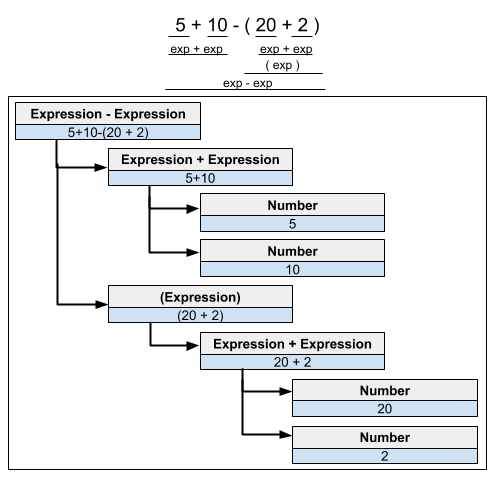
\includegraphics[scale=0.7]{Diagrams/syntaxTree.png}
		
		\caption{Diagram syntax tree for an expression.} \label{syntax tree}
	}
\end{figure}
\FloatBarrier

\noindent
Similar to the scanner, the parser program can be quite complex. It needs to find the associated terminal and non-terminal symbols and comply with the grammatical model. Furthermore, if there is a change in the grammar or there is a need to add features at a later date, it is frequently difficult to change the parser. Many studies have been conducted on creating a parsers; however this is beyond the scope of this thesis. Therefore, a program called a parser generator can be used to create the parser program. It uses a specification of the grammar similar to that of the \acrshort{bnf} to generate a C program capable of parsing a given language. A popular implementation of a parser generator is called Bison.

\subsection{\acrlong{bnf} of the L-system Grammar} \label{L-system Grammar}

A \acrshort{bnf} below is used to describe any possible valid L-system. The Bison program takes a definition similar to this one and creates the parser program. The parser takes in an L-system as input and will process and output the appropriate data structures and information necessary to carry out rewriting.

\begin{singlespace}
	\begin{bnf*}
	\bnfprod{lSystem}
		{\bnfes \bnfor \bnfpn{statements} \bnfsp \bnfts{EOF}}\\
	\bnfprod{statements}
		{\bnfes \bnfor \bnfpn{statement} \bnfpn{statements}}\\
	\bnfprod{statement}
		{\bnfts{EOL} \bnfor \bnfpn{generation} 
		\bnfor \bnfpn{definition} 
		\bnfor \bnfpn{object} 
		\bnfor \bnfpn{axiom} 
		\bnfor \bnfpn{production}}\\
	\bnfprod{generation}
		{\bnfts{\#define} \bnfsp \bnfts{=} \bnfsp \bnfpn{float} \bnfts{;}}\\
	\bnfprod{float}
		{\bnfts{[0-9]+.[0-9]+$|$[0-9]+}}\\
	\bnfprod{variable}
		{\bnfts{[a-zA-Z\_][a-zA-Z0-9\_]*}}\\
	\bnfprod{number}
		{\bnfpn{float} \bnfor \bnfts{-} \bnfsp \bnfpn{float}}\\
	\bnfprod{range}
		{\bnfts{\{} \bnfpn{number} \bnfts{,} \bnfpn{number} \bnfts{\}}}\\
	\bnfprod{definition}
		{\bnfts{\#define} \bnfsp \bnfpn{variable} \bnfsp \bnfpn{number} \bnfts{;}}\\
	\bnfprod{object}
		{\bnfts{\#object} \bnfsp \bnfpn{variable} \bnfsp \bnfpn{variable} \bnfts{;}}\\ 
	\bnfprod{module}
		{\bnfpn{variable} \bnfor \bnfts{+} 
		\bnfor \bnfts{-} 
		\bnfor \bnfts{/} 
		\bnfor \bnfts{$\backslash$} 
		\bnfor \bnfts{$\land$}
		\bnfor \bnfts{\&}
		\bnfor \bnfts{\$}
		\bnfor \bnfts{[}
		\bnfor \bnfts{]}
		\bnfor \bnfts{!}}\\
		\bnfmore{\bnfor \bnfts{+} \bnfts{(} \bnfpn{param} \bnfts{,} \bnfsp \bnfpn{paramList} \bnfts{)}}\\
		\bnfmore{\bnfor \bnfts{-} \bnfts{(} \bnfpn{param} \bnfts{,} \bnfsp \bnfpn{paramList} \bnfts{)}}\\
		\bnfmore{\bnfor \bnfts{/} \bnfts{(} \bnfpn{param} \bnfts{,} \bnfsp \bnfpn{paramList} \bnfts{)}}\\
		\bnfmore{\bnfor \bnfts{$\backslash$} \bnfts{(} \bnfpn{param} \bnfts{,} \bnfsp \bnfpn{paramList} \bnfts{)}}\\
		\bnfmore{\bnfor \bnfts{$\land$} \bnfts{(} \bnfpn{param} \bnfts{,} \bnfsp \bnfpn{paramList} \bnfts{)}}\\
		\bnfmore{\bnfor \bnfts{\&} \bnfts{(} \bnfpn{param} \bnfts{,} \bnfsp \bnfpn{paramList} \bnfts{)}}\\
		\bnfmore{\bnfor \bnfts{\$} \bnfts{(} \bnfpn{param} \bnfts{,} \bnfsp \bnfpn{paramList} \bnfts{)}}\\
		\bnfmore{\bnfor \bnfts{[} \bnfts{(} \bnfpn{param} \bnfts{,} \bnfsp \bnfpn{paramList} \bnfts{)}}\\
		\bnfmore{\bnfor \bnfts{]} \bnfts{(} \bnfpn{param} \bnfts{,} \bnfsp \bnfpn{paramList} \bnfts{)}}\\
		\bnfmore{\bnfor \bnfts{!} \bnfts{(} \bnfpn{param} \bnfts{,} \bnfsp \bnfpn{paramList} \bnfts{)}}\\
	\bnfprod{axiom}
		{\bnfts{\#w} \bnfsp \bnfts{:} \bnfsp \bnfpn{axiomStatementList} \bnfts{;}}\\
	\bnfprod{axiomStatementList}
		{\bnfes \bnfor \bnfpn{axiomStatement} \bnfpn{axiomStatementList}}\\
	\bnfprod{axiomStatement}
		{\bnfpn{module}}\\
	\bnfprod{paramList}
		{\bnfes \bnfor \bnfpn{param} \bnfpn{paramList}}\\
	\bnfprod{param}
		{\bnfpn{expression}}\\
	\bnfprod{expression}
		{\bnfpn{variable} \bnfor \bnfpn{number} \bnfor \bnfpn{range}}\\
		\bnfmore{\bnfor \bnfpn{expression} \bnfts{+} \bnfpn{expression}}\\
		\bnfmore{\bnfor \bnfpn{expression} \bnfts{-} \bnfpn{expression}}\\
		\bnfmore{\bnfor \bnfpn{expression} \bnfts{*} \bnfpn{expression}}\\
		\bnfmore{\bnfor \bnfpn{expression} \bnfts{/} \bnfpn{expression}}\\
		\bnfmore{\bnfor \bnfpn{expression} \bnfts{$\land$} \bnfpn{expression}}\\
		\bnfmore{\bnfor \bnfts{(} \bnfpn{expression} \bnfts{)}}\\
	\bnfprod{production}
		{\bnfts{\#} \bnfpn{variable} \bnfsp \bnfts{:} \bnfsp \bnfpn{predecessor} \bnfsp \bnfts{:} \bnfsp \bnfpn{condition} \bnfsp \bnfts{:} \bnfsp \bnfpn{successor} \bnfts{;}}\\
		\bnfprod{predecessor}
		{\bnfpn{predecessorStatementList}}\\
	\bnfprod{predecessorStatementList}
		{\bnfes \bnfor \bnfpn{predecessorStatement} \bnfpn{predecessorStatementList} }\\
	\bnfprod{predecessorStatement}
		{\bnfpn{module}}\\
	\bnfprod{condition}
		{\bnfts{*}}\\
		\bnfmore{\bnfor \bnfts{$\sim$} \bnfpn{float}}\\
		\bnfmore{\bnfor \bnfpn{leftExpression} \bnfpn{operator} \bnfpn{rightExpression}}\\
	\bnfprod{leftExpression}
		{\bnfpn{expression}}\\
	\bnfprod{rightExpression}
		{\bnfpn{expression}}\\
	\bnfprod{operator}
		{\bnfts{==} \bnfor \bnfts{!=} \bnfor \bnfts{$<=$} \bnfor \bnfts{$>=$} \bnfor \bnfts{$>$} \bnfor \bnfts{$<$}}\\
	\bnfprod{successor}
		{\bnfpn{successorStatementList}}\\
	\bnfprod{successorStatementList}
		{\bnfes \bnfor \bnfpn{successorStatement} \bnfpn{successorStatementList}}\\
	\bnfprod{successorStatement}
		{\bnfpn{module}}\\
	\end{bnf*}

\newpage

\end{singlespace} 

\noindent
As seen above in the \acrshort{bnf} notation for a L-system, the goal state is $<$lSystem$>$. The $<$lSystem$>$ can be made up of $<$statements$>$ beginning with the symbol \say{\#} and ending with the symbol \say{;}, or the \acrlong{eof} (\acrshort{eof}) character signifying the end of the L-system. Each non-terminal $<$statements$>$ is made up of a $<$statement$>$ followed by more $<$statements$>$, or an empty string ($\epsilon$). The $<$statement$>$ itself can either be an \acrlong{eol} (\acrshort{eol}) character or a $<$generation$>$, $<$definition$>$, $<$object$>$, $<$axiom$>$ or $<$production$>$ statement. The non-terminal symbols $<$float$>$ and $<$variable$>$ specify a regular expression. Each statement then has a number of terminal and non-terminal derivatives that allow the production of all valid L-systems that follow this grammar. 

In the previous chapter, the scanner defined the syntactic categories. These syntactic categories are all the valid terminal symbols within the L-system grammar. In essence, the parser takes these syntactic categories and finds if they fit the above \acrshort{bnf}, and if so, it extracts the information from the L-system and generates the relevant data structures and syntax tree. 

\subsection{Dealing with Constant Values and Objects} \label{constants subsection}

Defining constants and objects is essential as it allows the specification of named variables and module names that have a particular meaning. To define a constant or an object is syntactically similar. The keyword define or include is used, then a variable name followed by a value. The value for a constant is a floating-point number, and the value for an \textit{include} is a name of an object within the predefined object library. Seen below is an example of defining a constant and an object: 

\begin{equation} \label{constant and object example}
\begin{aligned}
	&\text{\#define num 10;}\\
	&\text{\#define pi 3.1415;}\\
	&\\
	&\text{\#include F BRANCH;}\\
	&\text{\#include S SPHERE;}\\
\end{aligned}
\end{equation}

\noindent
The definition variables can be stored as a table, called a constants table, which keeps track of all of the constant variable names as well as their values defined by the L-system, as seen in the table below: 

\begin{table}[h!] \center
\begin{tabular}{ | c | l | }
\hline
	Variable Name 	& Value\\  
\hline
\hline
	num 				& 10.0\\
\hline
	pi					& 3.1415\\
\hline
\end{tabular}
\caption{Table of turtle instruction symbols and their meaning to the interpreter}
\label{constants table}
\end{table}
\FloatBarrier

\noindent
The object table structure is very similar to the constants table. The object table holds the module name, and name of the object in the predefined object library. The object table is not used during rewriting, but it is necessary to provide information during the interpretation of the resulting string. 

\begin{table}[h!] \center
\begin{tabular}{ | c | l | }
\hline
	Module Name	& Object Name\\  
\hline
\hline
	F 				& BRANCH\\
\hline
	S				& SPHERE\\
\hline
\end{tabular}
\caption{Table of turtle instruction symbols and their meaning to the interpreter}
\label{constants table}
\end{table}
\FloatBarrier

\subsection{Implementing Modules and Strings} \label{modules and strings}

For the rewriter, it is crucial to understand that there are three significant parts of a module. There is a module name, which is a symbol or string of symbols. Secondly, there is a list of zero or more parameters signified by the open and close parenthesis. If there are no parameters for a module, it can be specified without parenthesis. However, if there are no parameters, there should then be a space between the current module and the next module. Thirdly, each parameter can either contain a number, variable, random number range, or a mathematical expression containing numbers, variables, and parentheses signifying precedence. 

It is important to note that there are two types of modules. One being a module definition and the other a module call. Although these are two different types of modules, they can refer to the same thing. The module definition stands as a template for a module within a production rule. These templates do not have to hold actual values but rather the variable names or random ranges, which will be substituted during the rewriting process. Module calls, on the other hand, would appear either in the axiom or in the resultant string. The parameters of a module call will always hold actual numerical values. Below is an example outlining the difference between the module definition and module calls.

\begin{equation} \label{module definition and call example}
\begin{aligned}
	&\text{\#w : A(10, 20);}\\
	&\text{\#p1 : A(x, y) : * : A(x+y, y); }\\
\end{aligned}
\end{equation}

\noindent
In the example \ref{module definition and call example} above, module A(10, 20) within the axiom is a module call, as it contains two numerical values of 10 and 20. In the production rule p1, the predecessor is the module A(x, y), this is a module definition, it states that module A's first parameter has a local variable x, and its second parameter has the local variable y. The calling modules values 10 and 20 will substitute x and y anywhere within the successor statement. The production rule p1's successor has a single module A(x+y, y). This is also a module definition; however, the variables will be substituted during rewriting with the calling modules value. When substituted, the successor will be A(10+20, 20). This module can be further evaluated to A(30, 20). After the successor module has been substituted and evaluated, the successors' modules must have a numerical value. They then become module calls within the resultant string ready for the next stage of rewriting.

A string in the context of a parametric L-system is a list of modules. The modules are linked one after the other, creating a type of string.

\subsection{Implementing Arithmetic Expressions Trees} \label{expression tree}

As stated previously within the L-system \acrshort{bnf}, an expression is either a variable name, a number, or a random range. It is also possible that an expression is part of another expression. Take the example: $5 \times 4 + n$, here there are three expressions 5, 4 and $n$ however, $5 \times 4$ is also an expression, as well as $4 + n$. An expression can also be described as any of the expressions above between a set of parentheses, such as $(4+n)$. The result of the expression is calculated from left to right unless parentheses are used, which prioritises the encapsulated expression to be calculated first. We can represent this expression as an expression tree in the diagram below:


\begin{figure}[htbp]
	{\centering
		\setlength{\fboxrule}{1pt}
		\vspace{7px}
		\fbox{
			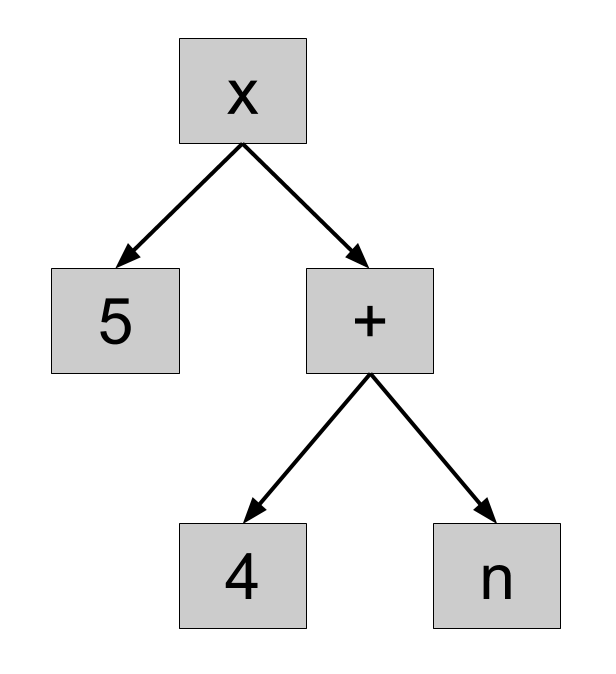
\includegraphics[scale=0.4]{Diagrams/ThesisContent.png}
		}
		\caption{Diagram of an expression tree.} \label{3D rotations}
	}
\end{figure}
\FloatBarrier

\noindent
The parser provides a syntax tree, which makes it easy to generate the above expression tree. The expression tree can be made up od four types of nodes: a variable, number, random range, or an operator. The leaf nodes of the expression tree must be either a number, variable or random range; moreover, a connecting node within the tree must be an operator. We can then traverse the generated tree and replace the variables with their associated value. For random ranges, the random value can be generated and assigned to the node. A second traversal during the rewriting process can then computes the result of the expression.

\subsection{Implementing Random Ranges} \label{random range}

L-systems are limited in the amount of variation they produce during the rewriting stage. In nature, the variation between the two plants depends on an enormous number of factors. These factors ultimately create variation within the branching structure and in the features of the branches, leaves, and flowers. These features include but are not limited to, branching angles, width, length, height, and weight. When introducing variation in the L-system branching structure, there must be randomness in how rules are chosen. This topic is discussed in section \ref{stochastic rules}. However, this section introduces a method of providing variation in the features of branch segments, called random ranges.

A random range is a method of declaring a variable that represents a number that is randomly generated between two bounding numbers. The bounding numbers are the minimum and a maximum, respectively. The primary method used for generating a pseudo-random number using a uniform distribution within a range can be seen below. 

\begin{singlespace}
\begin{algorithm}
\begin{algorithmic}[1]
\Procedure{Random Range}{min, max}
	\State n $\gets$ (rand() \% (max - min + 1)) + min
	\State \textbf{return} n
\EndProcedure
\end{algorithmic}
\end{algorithm}
\end{singlespace}

\noindent
Several other types of pseudo-random number generators could generate numbers according to different distributions, such as normal, binomial, Poisson, among others. When generating plant-life, a uniform distribution should be sufficient for most features and plant-life.

A random range can be declared in three different places within the L-system. It can be declared in the define statement, as an axiom parameter, or a production rule successor parameter. If the random range is declared within a define statement or the axiom, it will generate the random value during the parsing stage. However, if the range is defined in the successor, the number is generated during the rewriting process. More specifically, it is generated when the expressions within the successors are being evaluated. The values are generated during the rewriting process, rather than during parsing because each time a module is rewritten, the number should be a new random number. Generating the numbers during parsing means that the random number is only generated once, and then kept for use later. Conversely, generating the number during rewriting means that a new number will be generated every time rewriting takes place. 

\subsection{Implementing Stochastic Rules} \label{stochastic rules}

The term \say{stochastic} refers to a randomly determined process. This could be by a uniform distribution or some random probability distribution. 

One of the important factors of generating plant-life is being able to simulate randomness in the generation process. Section \ref{random range} covers a method of generating random numbers that can be used for the features within an L-system. This section covers a different type of randomness that affects the way the rewriter selects a rule for rewriting. In this way, rules can be selected randomly instead of meeting certain conditions. Randomly selecting rules provides randomness within the structure of the plant-life rather than the features.

In order to achieve stochastic rules, each rule must belong belonging to a stochastic group of rules that provides a probability value. The probability indicates how likely it is that rule is selected during the rewriting process. For production rules to be part of the same stochastic group, they are required to meet the following four criteria: 

\begin{itemize}
\item The stochastic operator $\sim$ must be used with a probability between 0.0 and 1.0.
\item The predecessor module name must match the other predecessor module names within that stochastic group.
\item The number of parameters within the predecessor must match the number of parameters of other production rules within that stochastic group.
\item The total probability of all of the production rules within the stochastic group must not exceed 1.0 or be less than 0.0.
\end{itemize}

\noindent
During the parsing phase, if the rule has the stochastic operator, the probability of the rule must be kept for later use within a stochastic probability table. The table also keeps track of which rules are associated with which stochastic groups. A stochastic probability table can be generated from the rules below, as seen in table \ref{stochastic table}. 

\begin{equation} \label{stochastic implementation example}
\begin{aligned}
	&p_1~ :  F(x)~ :~ \sim 0.33 ~ :~ F(x)[+(r)F(x)]F(x)[-(r)F(x)]F(x)\\
	&p_2~ :  F(x)~ :~ \sim 0.33 ~ :~ F(x)[+(r)F(x)]F(x)\\
	&p_3~ :  F(x)~ :~ \sim 0.34 ~ :~ F(x)[-(r)F(x)]F(x)\\
\end{aligned}
\end{equation}

\begin{table}[h!] \center
\begin{tabular}{ | c | c | c | }
\hline
	Stochastic Group & Rule Name & Probability\\  
\hline
\hline
\multirow{3}{*}{F1} & p1 & 0.33 \\
& p2 & 0.33 \\
& p3 & 0.34 \\
\hline
\end{tabular}
\caption{Table of the stochastic rules probabilities within a stochastic group.}
\label{stochastic table}
\end{table}
\FloatBarrier

The stochastic name used within the stochastic table is generated by using the predecessor module name in the production rule, as well as the number of parameters within the predecessor module. In the example above, we can use the predecessor name F, which has a single parameter, making the stochastic name F1. This method of naming serves as a unique identifier for the stochastic group. Once all of the production rules are processed, each groups' probabilities are added together. The total probability should equal 1.0. A tolerance should put in place to account for floating-point error.

During the rewriting process, the module that is being rewritten is matched to a particular stochastic group. A uniformly distributed random number is generated between 0.0 and 1.0. A range for each rule is generated, for instance, p1 will be between 0.0 and 0.33, p2 will be between 0.33 and 0.66, and finally, p3 will be between 0.66 and 1.0. The production rule will be chosen where the random number falls between. For example, if the random number is 0.456, p2 will be chosen as 0.456 falls between 0.33 and 0.66.

\section{The String Rewriter}

Once the L-system has been processed by the lexical analyser and the parser, the L-systems' resulting data structures are ready for string rewriting. All of the data structures necessary for rewriting can be seen in the list below. A definition of these data structures can be seen in appendix \ref{rewriter data structures}.

\begin{singlespace}
\begin{itemize}
	\item Constant variables table
	\item Local variable table
	\item Number of generations
	\item Production rules
	\begin{itemize}
		\item Predecessor module
		\item Condition or stochastic probability
		\item Successor string of modules
	\end{itemize}
	\item Axiom string of modules
\end{itemize}
\end{singlespace}

\noindent
The string rewriter is the final stage in the rewriter system. It starts with the axiom as the current string of modules. It then iterates over each module within the current string, matching it to the production rules. If the module matches a rule, the modules' parameter values are matched to the predecessors' parameter variable names and stored in the local variable table. The variables in the production rules successor are replaced according to the constant and local variable tables and subsequently evaluated. The production rule successor is then stored in a result string. If a match is not found, the module itself is stored in the result string. Once all the modules have been rewritten, the result string replaces the current string, and the local table is emptied. This process is carried out for the number of generations specified by the L-system and will eventually provide the final result string of modules. The pseudocode for the rewriting procedure, as well as several useful functions, can be found in appendix \ref{rewriter pseudocode} for more detail. 

\section{Summary}

The L-system rewriter is the first of two major systems within the process of procedurally generating plant-life. The second system is the interpreter. The rewriters' purpose is to take an L-system input and understand its grammatical structure and carry out string rewriting.

The rewriter system defined in this thesis acts as a type of compiler, which is similar to a computer language. The L-system becomes a type of language that the L-system rewriter can understand. This understanding allows the creation of data structures, which allow the rewriting process to be carried out. The lexical analysis stage and the parser stage, give informative messages if there is a mistake, either grammatically or syntactically. If the language meets all of the grammatical and syntactic requirements, the rewriter can use this data to generate the resultant string of modules. The result string produced by the rewriting system will always be a valid string according to the L-system grammar. 

The L-system languages can be used for many different applications and are not limited to that of procedural plant generation. The interpreter uses the resultant string to create the final rendered representation, such as the plant model. The advantage of having the rewriter be complex is that the rewriting system does not need to change, even if the L-system is used for a different purpose.  Only the interpretation will need to change in order to understand the resulting string. This is the main reason behind using a compiler-like process to govern the string rewriting. It allows the L-system enough complexity to provide information to the interpreter, but not so much that interpretation becomes reliant on the string rewriter.

\chapter{Mathematics For 3D Graphics} \label{maths chapter}

In any 3D application, mathematical models are used to represent the positions, rotations and scale of objects within a given scene. All objects within a 3D application are represented by a set of vertices or points, which can be represented with X, Y and Z coordinates. Three vertices can make up one triangle also called a face, multiple faces will then make up a whole 3D object. The use of mathematical methods in 3D graphics is to be able to manipulate all vertices of an object in a consistant way, thus rotating, translating or scaling the object within the scene. This section will provide sufficient background on some of most important concepts of 3D Mathematics, such as vectors, matrices and quaternions, which are widely used in the turtle graphics interpreter as well as the model generator.

\section{Vectors}

Vectors have many meanings in different contexts, in \acrshort{3d} computer graphics, often vectors are refering to the Euclidean vector. The Euclidean vector is a quantity in $n$-dimensional space that has both magnitude (the length from A to B) and direction (the direction to get from A to B). Vectors can be represented as a line segment pointing in a direction, with a certain length. A \acrshort{3d} vector can be written as a triple of scalar values eg: $(x, y, z)$

The most common operations on vectors are multiplication by a scalar, addition, subtraction, normalisation and the dot and cross product. The multiplication by a scalar value can be simply seen as scaling the magnitude of the vector itself, this can be done uniformly or non-uniformly as seen in the equation below:

\begin{equation}
a \otimes s = (a_x s_x, a_y s_y, a_z s_z)
\end{equation}

\noindent
Where $\otimes$ is the component-wise product of a vector $a$ and the scaling vector $s$. Similar to the scalar product of a vector the addition and subtraction of two vectors is the component-wise sum or difference. 

\begin{equation}
\begin{aligned}
a \oplus b = [(a_x + b_x), (a_y + b_y), (a_z + b_z)]\\
a \ominus b = [(a_x - b_x), (a_y - b_y), (a_z - b_z)]
\end{aligned}
\end{equation}

\begin{figure}[htbp]
	{\centering
		\setlength{\fboxrule}{1pt}
		\vspace{7px}
		\fbox{
			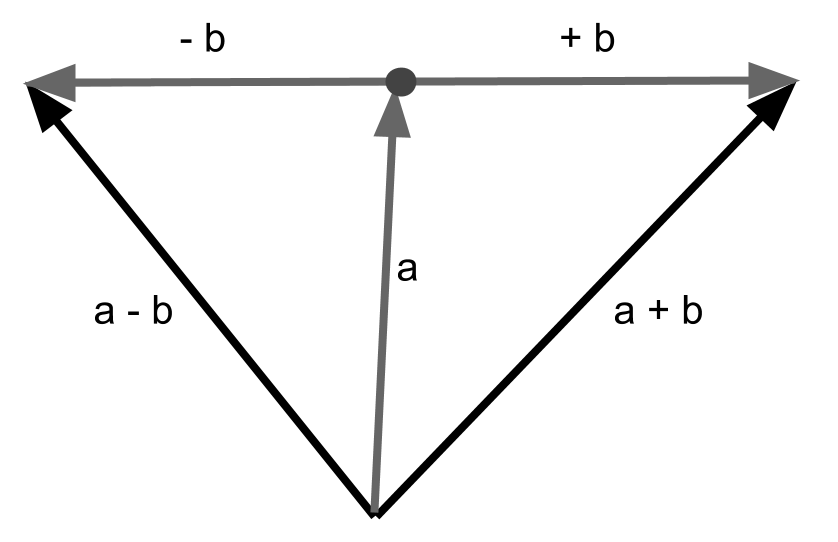
\includegraphics[scale=0.2]{Diagrams/vector_addition.png}
			\label{3DAxisFigure}
		}
		\caption{Table of common dot product tests between two vectors.}
	}
\end{figure}
\FloatBarrier

\noindent
A useful type of vector is known as a unit vector. This is a type of vector which has a magnitude of 1. Unit vectors are used extensively in computer graphics particularly with ragards to \gls{Shader}s. Take the vector v its magnitude $\alpha$ can be calculated by taking the square root of the product its components squared, as seen below 

\begin{equation}
	\alpha =~ \mid \textbf{v} \mid~ = \sqrt{\textbf{v}^2_x + \textbf{v}^2_y + \textbf{v}^2_z}
\end{equation}

The unit vector can then be calculated by taking the product of $v$ and the reciprocal of its magnitude shown in the following equation.

\begin{equation}
	\upsilon = \frac{\textbf{v}}{\alpha} = \frac{1}{\alpha} \textbf{v}
\end{equation}

There are many different ways to multiply vectors, however, in 3D graphics there two main multiplications. These being the dot and cross product. The dot product yields a scalar by adding the products of the vector product components. The cross product on the other hand is the product of two vectors which gives a vector which is perpendicular. The dot product can be calculated using the formula below: 

\begin{equation}
a \cdot b = a_x b_x + a_y b_y + a_z b_z = d
\end{equation}

\noindent
Some of the main uses for dot products within 3D graphics is to find whether two vectors are collinear, perpendicular, in the same direction or opposite directions. One possible use for this is to find the dot product of two branches directions in order to find out if they growing in the same direct or in opposite directions. In the table \ref{dot product test} below, there are each of the dot product test diagrams as well as the test equation where $ab = \mid a \mid \mid b \mid = a \cdot b$.

\begin{table}[h!]
\centering
\begin{tabular}{ | c | c | c |}
\hline
	Test 	& Equation & Example\\  
\hline
\hline
	Collinear 							& $(a \cdot b) = ab$ & 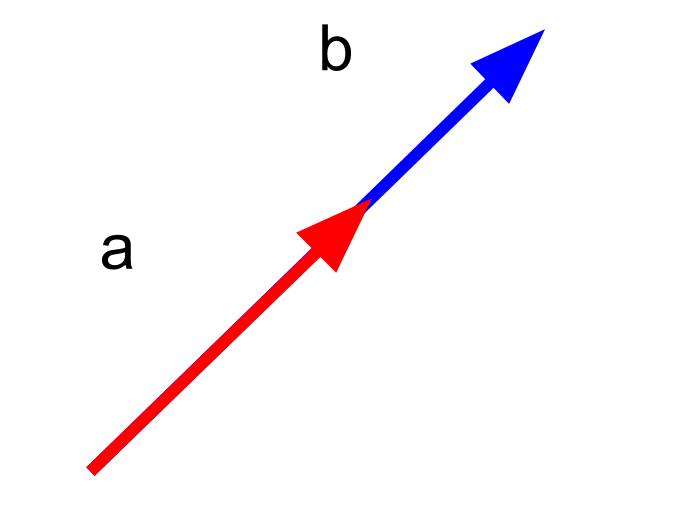
\includegraphics[scale=0.1]{Diagrams/vector1.png}\\
\hline
	Opposite Collinear 					& $(a \cdot b) = -ab$ &	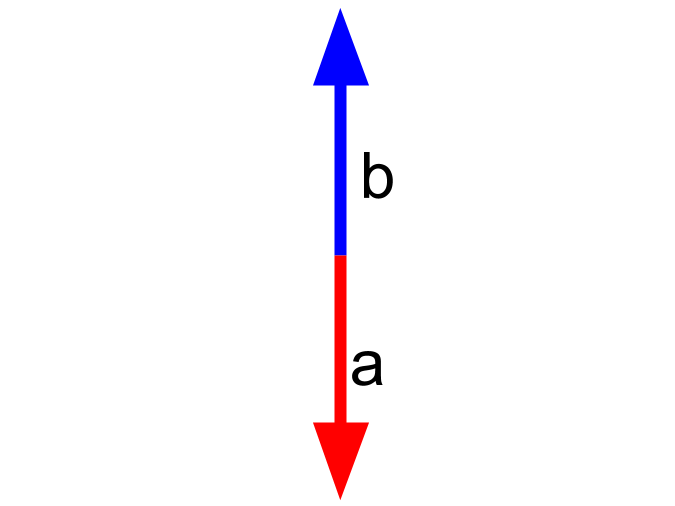
\includegraphics[scale=0.1]{Diagrams/vector2.png}\\
\hline
	Perpendicular 						& $(a \cdot b) = 0$	&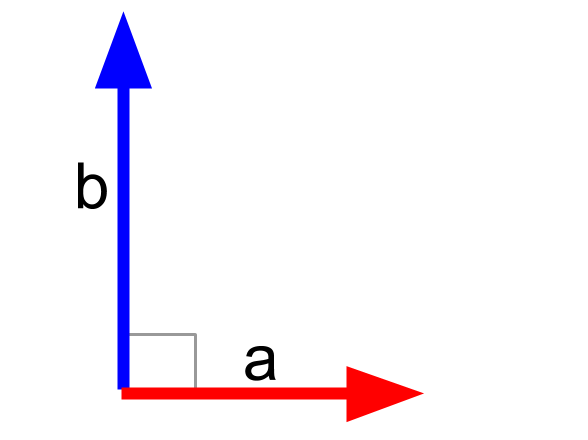
\includegraphics[scale=0.1]{Diagrams/vector3.png}\\
\hline
	Same Direction 						& $(a \cdot b) > 0$ &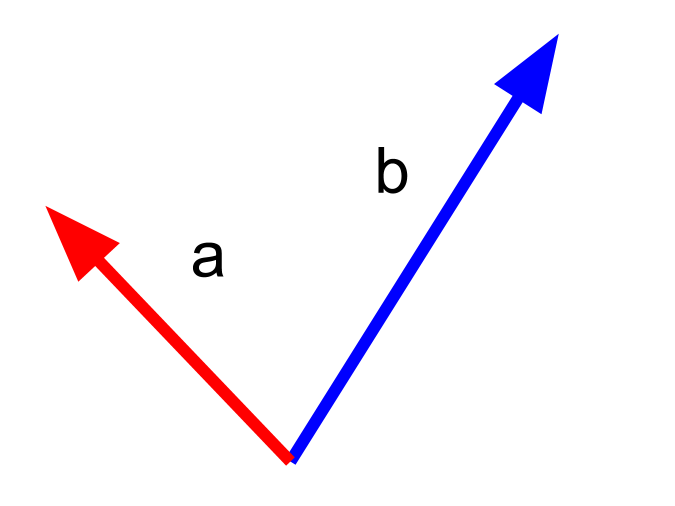
\includegraphics[scale=0.1]{Diagrams/vector4.png}\\
\hline
	Opposite Direction 					& $(a \cdot b) < 0$ &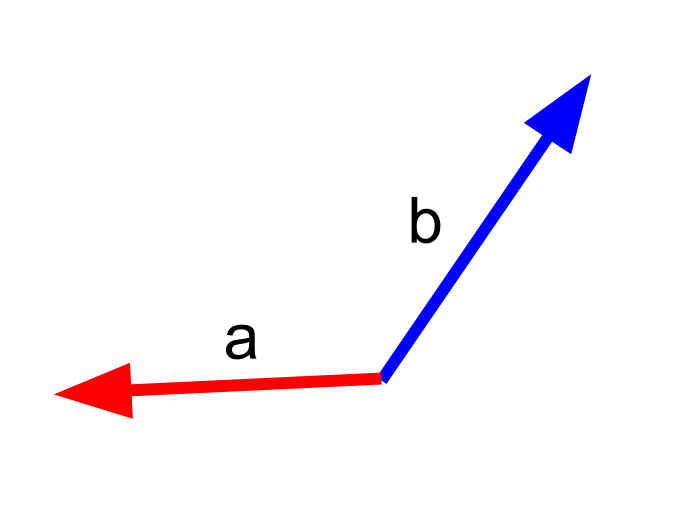
\includegraphics[scale=0.1]{Diagrams/vector5.png}\\
\hline

\end{tabular}
\caption{Table of turtle instruction symbols and their meaning to the interpreter}
\label{dot product test}
\end{table}
\FloatBarrier

\noindent
The cross product also known as the outer product takes two vectors and finds the perpendicular vector of the two vectors, this is only possible in 3D space and can be expressed in the following formula using the left-hand rule: 

\begin{equation}
a \times b = [(a_y b_z - a_z b_y), (a_z b_x - a_x b_z), (a_x b_y - a_y b_x)]
\end{equation}

\noindent
The result of a cross product can be seen in figure \ref{Cross product diagram} below. Where vectors $a$ and $b$ give the perpendicular vector $a \times b$. The cross product is very useful within physics calculations when it is necessary to find the rotational motion. 

\noindent
Some of the properties of the cross product are as follows:

\begin{itemize}
	\item is non-commutative, meaning order matters($a \times b \not= b \times a$).
	\item is anti-commutative ($a \times b = -(a \times b)$).
	\item is distributive with addition ($a \times (b + c) = (a \times b) + (a \times c)$).
\end{itemize}

\begin{figure}[htbp]
	{\centering
		\setlength{\fboxrule}{1pt}
		\vspace{7px}
		\fbox{
			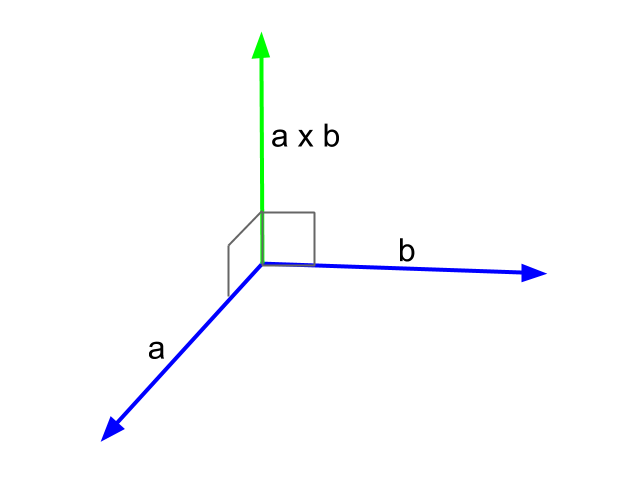
\includegraphics[scale=0.25]{Diagrams/cross_product.png}
			\label{Cross product diagram}
		}
		\caption{Diagram of the cross product of two vectors a and b.}
	}
\end{figure}
\FloatBarrier

\section{Matrices}

A model in 3D space will exist as a set of vertices which each have a position. Moving the model requires moving all of the the vertices of that model without distorting it in any way, this is called a model transform. There are four main types of transforms; translation, rotation, scale and shear. Matrices are a single matematical construct which is capable of carrying out all four of these transformations. This sections will only cover the first three as the shear transformation is likely not going to be useful for this thesis.    

A matrix is an 2D array of numbers, arranged into rows and columns, which can come in many different sizes. In 3D graphics, matrices used for transformations are the 3 $\times$ 3 and 4 $\times$ 4 matrix as seen below. A 3 $\times$ 3 matrix can be used for linear transorms such as scaling and rotation, furthermore, a linear transform which contains translation is known as an affine transform and can be represented by a 4 $\times$ 4 matrix known as an Atomic Transform Matrix. An atomic Transfom matrix is the concatination of four 4 $\times$ 4 matrices, one for translations, rotations, scale and shear transforms. Resulting in a 4 $\times$ 4 matrix as shown below. 

\begin{equation}
\textbf{M} = \begin{bmatrix}
M_{11} & M_{12} & M_{13} \\
M_{21} & M_{22} & M_{23} \\
M_{31} & M_{32} & M_{33}
\end{bmatrix}
\end{equation}

\begin{equation}
\textbf{M} = \begin{bmatrix}
M_{11} & M_{12} & M_{13} & M_{14}\\
M_{21} & M_{22} & M_{23} & M_{24}\\
M_{31} & M_{32} & M_{33} & M_{34}\\
M_{41} & M_{42} & M_{43} & M_{44}
\end{bmatrix}
\end{equation}

\noindent
The affine matrix can be shown in the expression below where $RS$ is a 3 $\times$ 3 matrix containing the rotation and scale where the $4^th$ elements are 0. The $T$ elements represent the translation with the 4th element being 1. 

\begin{equation}
\textbf{M} = \begin{bmatrix}
RS_{11} & RS_{12} & RS_{13} & 0\\
RS_{21} & RS_{22} & RS_{23} & 0\\
RS_{31} & RS_{32} & RS_{33} & 0\\
T_{1} & T_{2} & T_{3} & 1
\end{bmatrix}
\end{equation}

The product of two linear transform matrices will be another linear transform matrix that carries out both of those tranformations. This is true for the multiplication of two affine transform matrices as well, and is why matrix multiplication is so powerful in 3D graphics. Take the two matrices $A$ and $B$ which give the product $P$. In order to multiply $A$ and $B$ together, the dot product of the row and the column is calculated as seen below. It is also imporant to know that matrix multiplication is non-commutative $(AB \not= BA)$.

\begin{equation}
\textbf{AB} = \begin{bmatrix}
A_{11} & A_{12} & A_{13}\\
A_{21} & A_{22} & A_{23}\\
A_{31} & A_{32} & A_{33}
\end{bmatrix}
\times
\begin{bmatrix}
B_{11} & B_{12} & B_{13}\\
B_{21} & B_{22} & B_{23}\\
B_{31} & B_{32} & B_{33}
\end{bmatrix}
= \begin{bmatrix}
(A_{row1} \cdot B_{col1}) & (A_{row1} \cdot B_{col2}) & (A_{row1} \cdot B_{col3})\\
(A_{row2} \cdot B_{col1}) & (A_{row2} \cdot B_{col2}) & (A_{row2} \cdot B_{col3})\\
(A_{row3} \cdot B_{col1}) & (A_{row3} \cdot B_{col2}) & (A_{row3} \cdot B_{col3})
\end{bmatrix}
\end{equation}

To translate a vertex in 3D space without causing any distortion. The vertex can be added the the matrix below as follows. These translations can be carried out on all vertices in order to translate a whole object model. 

\begin{equation}
V + T = \begin{bmatrix}
V_{x} \\
V_{y} \\
V_{z}~ \\
1
\end{bmatrix}
+
\begin{bmatrix}
1 & 0 & 0 & 0\\
0 & 1 & 0 & 0\\
0 & 0 & 1 & 0\\
T_{x} & T_{y} & T_{z} & 1
\end{bmatrix}
= \begin{bmatrix}
(V_x + T_x)~ \\
(V_y + T_y)~ \\
(V_z + T_z)~ \\
1
\end{bmatrix}
\end{equation}

\noindent

In order to rotate a vertex in 3D space the vertex position and the rotation angle can be applied to the as a matrix depending on the axis about which it is rotating. These rotation matrices can be applied to the vertex itself in order to gain the new position of the vertex. 

\begin{equation}
R_x(\theta) = 
\begin{bmatrix}
(v_x)~ \\
(v_y)~ \\ 
(v_z)~ \\
1
\end{bmatrix}
\begin{bmatrix}
1 	& 0 					& 0 					& 0\\
0 	& \text{cos}(\theta) 	& \text{sin}(\theta) 	& 0\\
0 	& -\text{sin}(\theta) 	& \text{cos}(\theta) 	& 0\\
0 	& 0 					& 0 					& 1
\end{bmatrix}
\end{equation}

\begin{equation}
R_y(\theta) = 
\begin{bmatrix}
(v_x)~ \\
(v_y)~ \\
(v_z)~ \\
1
\end{bmatrix}
\begin{bmatrix}
\text{cos}(\theta) 	& 0 					& -\text{sin}(\theta) 	& 0\\
0 					& 1						& 0						& 0\\
\text{sin}(\theta) 	& 0 					& \text{cos}(\theta)	& 0\\
0 					& 0 					& 0 					& 1
\end{bmatrix}
\end{equation}

\begin{equation}
R_z(\theta) = 
\begin{bmatrix}
(v_x)~ \\
(v_y)~ \\
(v_z)~ \\
1
\end{bmatrix}
\begin{bmatrix}
\text{cos}(\theta) 	& \text{sin}(\theta) 	& 0						& 0\\
-\text{sin}(\theta) & \text{cos}(\theta) 	& 0
					& 0\\
0 					& 0 					& 1						& 0\\
0 					& 0 					& 0 					& 1
\end{bmatrix}
\end{equation}


\begin{equation}
ST = \begin{bmatrix}
S_{x} \\
S_{y} \\
S_{z} \\
1
\end{bmatrix}
\begin{bmatrix}
S_x & 0 & 0 & 0\\
0 & S_y & 0 & 0\\
0 & 0 & S_z & 0\\
0  & 0  & 0 & 1
\end{bmatrix}
= \begin{bmatrix}
(S_x R_x)~ \\
(S_y R_y)~ \\
(S_z R_z)~ \\
1
\end{bmatrix}
\end{equation}

\section{Quaternions}

In computer graphics there are a number of ways to represent 3D rotations. One method is to use matrix affine transforms, which is spoken about in the previous section. Matrices are a common way of represening rotation, however, it has a number of limitations. Matrices are represented by nine floating point values and can be computationally expensive to store and process, particularly when doing a vector to matrix multiplication. There are also situations where it is neccessary to smoothly interpolate from one rotation to another or to find the rotation somewhere between two different rotations. It is possible to make these calculations using matrices but it can become very complicated and even more computationally expensive. Quaterions are the answer to these challenges.

Quaternions look similar to a 4D vector. They contain four axes $q = [q_x, q_y, q_z, q_w]$, these are represented with a real axis ($q_w$) and three imaginary axes ($q_x, q_y, q_z$). A quaternion can be represented in the complex form below: 

\begin{equation}
q = (iq_x + jq_y + kq_z + qw)
\end{equation}

\noindent
For the purpose of this thesis it is not important to understand the derivation of quaterions in mathematics. However it is important to understand that any quaternion which obays the rule in \ref{unit quat} below is known as a unit quaternion.

\begin{equation} \label{unit quat}
	q_x^2 + q_y^2 + q_z^2 + q_w^2 = 1
\end{equation}

\noindent
Unit quaternions can be used for rotations, it is possible to convert a quaternion to a unit quaternion by taking the angle and the axis of a rotation and applying to the quaternion as seen in \ref{unit quat conversion}.

\begin{equation} \label{unit quat conversion}
\begin{aligned}
& q = [q_x, q_y, q_z, q_w]\\
& \text{where} \\
& q_x = a_x sin \frac{\theta}{2}\\
& q_y = a_y sin \frac{\theta}{2}\\
& q_z = a_z sin \frac{\theta}{2}\\
& q_w = cos \frac{\theta}{2}
\end{aligned}
\end{equation}

\noindent
The scalar part ($q_w$) is the cosine of the half angle, and the vector part ($q_x q_y q_z$) is the axis of that rotation, scaled by sine of the half angle of rotation. The unit quaternion can be used for rotations in a number of ways. The most useful of which is to rotate vectors, interpolate between two rotations and concatonate rotations together similar to how matrix transformations can be multiplied.

The first operation for quaternions is that of addition. The addition of two quaternions is quite simple, it involves taking each component of each quaternion and adding them together. This is similar to that of matrices addition and can be expressed as follows:

\begin{equation}
p + q = [(p_w + q_w), (p_x + q_x), (p_y + q_y), (p_z + q_z)]
\end{equation}

\noindent
Multiplication of quaternions is also incredibly powerful and can be used to concatonate rotations. There are a number of different types of quaternion multiplication, however, the one most commonly used for quaternion rotaton is called the grassmann product. This can be described in the following formula below. Where $p$ and $q$ are quaternions and the subscript $w$ indicates the scalar part and subscript $x, y, z$ indicate the vector components of each quaternion.

\begin{equation}
\begin{aligned}
& R = r_w + r_x + r_y + r_z\\
& \text{where}\\
& r_w = p_w q_w - (p_x q_x + p_y q_y + p_z q_z)\\
& r_x = p_w q_x + p_x q_w + p_y q_z - p_z q_y\\
& r_y = p_w q_y + p_y q_w - p_x q_z + p_z q_x\\
& r_z = p_w q_z + p_z q_w + p_x q_y - p_y q_x\\
\end{aligned}
\end{equation}

\noindent
To rotate a vector by a unit quaternion the vector will need to be converted into its quaternion form. This requires taking the unit vector $v$ and using it as the vector part of the quaternion with a scalar part being equal to zero. This can be written as $Q_v = [v, 0] = [v_x, v_y, v_z, 0]$. The grassmann product can be used to calculate the rotation, by taking the product of the rotation quaternion $q$ and the vector form quaternion $v$ and the inverse of the rotation quaternion $q^-1$. \\

\begin{equation}
	V_q = qvq^{-1}
\end{equation}

\noindent
For unit quaternions the conjugate and the inverse are identical. Quite simply the inverse of a unit quaternion can be calculated by negating the vector components of the quaternion whilst leaving the scalar component the same. This can be expressed as follows:

\begin{equation}
	q^{-1} = [-q_v, q_s]
\end{equation}

\noindent
Quaternion rotations can be concatonated together similar to how matrix transforms can be multiplied together in affine transforms. The grassman product is noncommutative and therefore order matters. Using the grassmann product the rotations can easily be multiplied together to give the result of all of those rotations as if they were to happen one after the other. This can be expressed as follows:

\begin{equation}
\begin{aligned}
Q_{net} = Q_3 Q_2 Q_1\\
v' = Q_3 Q_2 Q_1~ v~ Q_{1}^{-1} Q_{2}^{-1} Q_{3}^{-1}
\end{aligned}
\end{equation}

\noindent
The order by which the quaternions $Q_1, Q_2$ and $Q_3$ are applied is $Q_3$ then $Q_2$ and then $Q_1$. To apply this to a vector the product of the three quaternions is multiplied to the vector and then multiplied to the product of the inverse of each quaternion. 

Another incredibly useful mathematical function is called rotational linear interpolation also known as \acrshort{lerp}. The \acrshort{lerp} function takes two quaternions, $Q_1$ and $Q_2$ and linearly interperpolates between those two rotations by a given percentage  $\beta$. The \acrshort{lerp} function can be defined as follows.

\begin{equation}
\begin{aligned}
& Q_{\text{LERP}} = \text{LERP}(Q_1, Q_2, \beta) = \frac{(1-\beta)Q_1 + \beta Q_2}{\mid(1-\beta)Q_1 + \beta Q_2\mid} \\
& = \text{normalize} \left(\begin{bmatrix}
(1 - \beta) Q_{1x} + \beta Q_{2x}\\
(1 - \beta) Q_{1y} + \beta Q_{2y}\\
(1 - \beta) Q_{1z} + \beta Q_{2z}\\
(1 - \beta) Q_{1w} + \beta Q_{2w}					
\end{bmatrix}\right)
\end{aligned}
\end{equation}

\noindent
Using the linear interpolation function will result in a rotation between $Q_1$ and $Q_2$ at a given percentage $\beta$ that is between 0 and 1. Where 0 is the rotation of $Q_1$ and 1 is rotation of $Q_2$.

\section{summary}










\chapter{L-system String Interpreter Implementation} \label{interpreter implementation}

\lettrine[lines=3]{T}{}he string interpreter is one of the major components of plant generation and it is the final step in the process of procedural generation. The output of this stage of processing is dependant on what the L-system is representing, in this case it is responsible for interpreting the resulting string of modules provided by the L-system rewriter, and uses this to generate the 3D models, structures and data of the resulting plant, which is then rendered and simulated on the screen using the OpenGL framework. The generation of plant-life has three main stages, the first part consists of a turtle graphics interpreter which takes the string of modules as a set of instructions, it starts from the root of the tree and generates a skeleton made up of joints, this is similar to the techniques used in skeletal rigging in animation \cite{gregory2014game}. The joints within the tree skeleton each represents a branch segment which has some information about the properties of that segment. These segements can be used to generate the vertex, index and other data that make up the 3D models of the plant. These models can finally be passed to the final part of string interpreter which is the renderer, the renderer is reponsible for taking all the vertices, indices, textures and shaders and organising it in an optimal way that enables rendering the plant on the screen, as well as the physical simulation of the tree skeleton. The stages of string interpretation can be seen in figure \ref{l-system interpreter} below. 

\begin{figure}[htbp]
	{\centering
		\vspace{7px}
		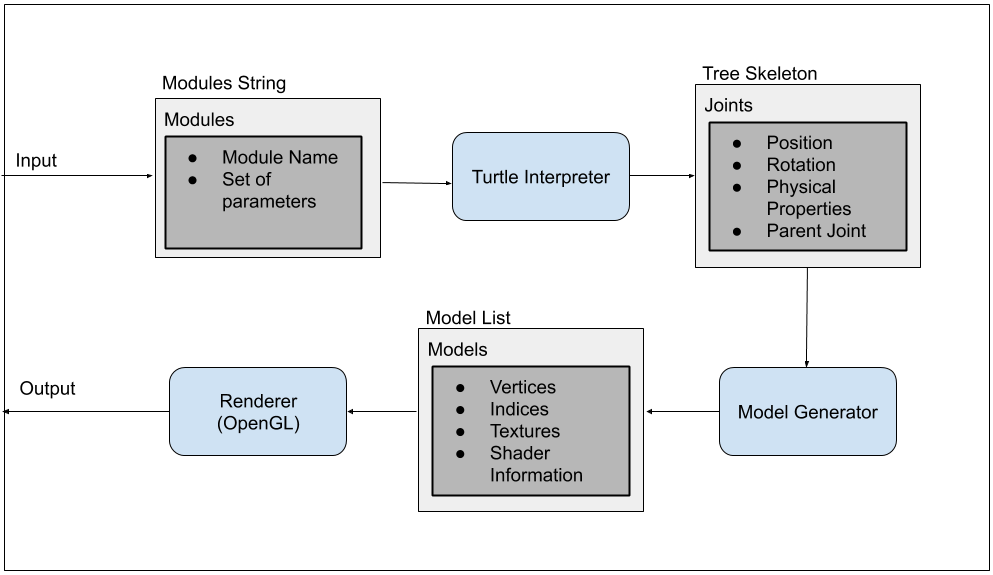
\includegraphics[scale=0.4]{Diagrams/L-systemInterpreter.png}
		\caption{Diagram of the stages of L-system interpretation and rendering} \label{l-system interpreter}
	}
\end{figure}
\FloatBarrier

\noindent
This chapter will cover each stage of the string interpreter implementation in detail, as well as well as talk about how the interpreter is able to simulate and animation the plants movements under forces such as gravity and wind in real time. 

\section{Turtle Graphics Interpreter}

The main purpose of the turtle graphics interpreter is to take the string of modules from the L-system rewriter, and interpret it as a list of turtle graphics instructions. As briefly covered in chapter \ref{l-system chapter}, each module name within the L-systems resultant string represents a particular meaning to the turtle graphics interpreter. The meaning of the module names are predefined in the string interpreter and are dependant on what the L-system is trying to represent. The L-system defined for this thesis is a parametric L-system, which allows each module to also provide a number of optional parameters. These may also carry a particular meaning for the interpreter. For instance the forward instruction or module name \say{F} can have three parameters. The value of the first parameter is the distance to move forward, this can also be seen as the length of the branch segment. The second and third parameter is the spring constant of the branch and the mass of the branch repectively. These give some information to the physics simulation in order to animate the plant. Below is a table describing the L-system module names as well as the parameter meanings for the turtle graphics interpreter.

\begin{table}[h!]
\centering
\begin{tabular}{ | c | l | l | l |}
\hline
	Instruction Name 	& Parameter 1 & Parameter 2 & Parameter 3 \\  
\hline
\hline
	F 							& Distance	& Spring Constant	& Branch Mass\\
\hline
	f 							& Distance	& Spring Constant	& Branch Mass\\
\hline
	+ 							& Angle of rotation &			&\\
\hline
	- 							& Angle	of rotation	&			&\\
\hline
	/ 							& Angle	of rotation	&			&\\
\hline
	$\backslash$ 				& Angle	of rotation	&			&\\
\hline
	$\land$ 					& Angle	of rotation	&			&\\
\hline
	\& 							& Angle	of rotation	&			&\\
\hline
	! 							& Branch width		&			&\\
\hline
\end{tabular}
\caption{Table of turtle instruction symbols and their meaning to the interpreter}
\label{instruction table 1}
\end{table}
\FloatBarrier

\noindent
Each modules instruction is carried out one by one to generate the plants skeletal structure, which is made up of joints. The joints hold information about the properties of each particular segement or object of the plant. The joints properties are the position, orientation, scale, parent joint as well as its physical characteristics. It is important to note that all of the scales and rotations must happen before the forward movement. As the rotations change the orientation of the brach and then the movement generates the joint itself. A joint is defined by the figure below:

\begin{figure}[htbp]
	{\centering
		\vspace{7px}
		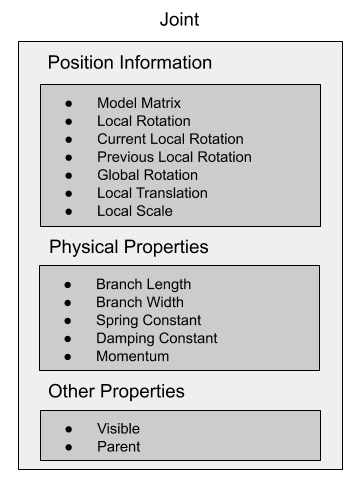
\includegraphics[scale=0.6]{Diagrams/JointDiagram.png}
		\caption{Diagram for the properties of a joint} \label{joint properties}
	}
\end{figure}
\FloatBarrier

\noindent
Figure \ref{joint properties} shows that there is in fact a large amount of information stored for the position and orientation of each joint. This is because the rotation of the joint is stored in both a local and global space. Local space refers to the rotation of the joint relative to its parent rotation, this is useful as it allows the manipulation of subsequent child joints, whilst leaving other joints local rotation unchanged. Global space, also known as world space, is the rotation of each joint relative to the world itself this is useful for understanding the current rotation of the joint relative to the world for instance calculating the torque or force calculations due to gravity. It is important to store both the current and previous rotations as they are used to calculate the rate of change for physics calculations.

The physical properties for each joint are the parts are what will affect model generation as well as physics simulations. These properties include the length, width, spring constant, damping constant as well as the current momentum of the branch. 

Take the following string of modules \say{F(1)[/(90)F(1)$\backslash$ (90)F(1)]-(90)F(1)+(90)F(1)}, the alphabet is made up of seven unique modules F, /, $\backslash$, [, ], + and -. According to the as discussed in previous chapters the \say{F} symbol represents a move forward, and \say{+}, \say{-}, \say{/}, \say{$\backslash$} symbolize different rotations, and the \say{[} and \say{]} represent save and load state respecively. The aforementioned symbols each have a single parameter except the load and save state. It is the turtle graphics interpreters job to understand what these parameters are and how to interpret them. In this case all of the \say{F} modules have the parameter value of 1, and all of the rotation modules have the parameter of 90. These are interpreted as the distance to move forward and the change in angle from the previous joint in degrees. This interpretation can be represented with the joint structure shown in figure \ref{skeleton diagram} below:

\begin{figure}[htbp]
	{\centering
		\vspace{7px}
		\setlength{\fboxrule}{1pt}
		\fbox{
			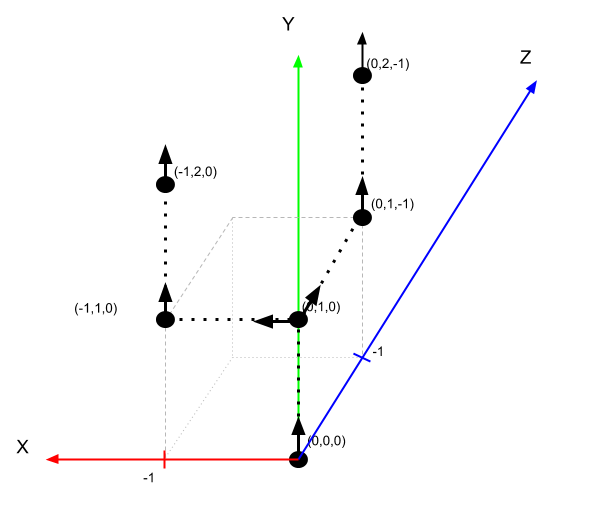
\includegraphics[scale=0.4]{Diagrams/SkeletonJoints.png}
		}
		\caption{Diagram of a simple plant skeleton with joint position and orientation.} \label{skeleton diagram}
	}
\end{figure}
\FloatBarrier


\section{3D Mathematics}

In any 3D application, mathematical models are used to represent the positions, rotations and scale of objects within a given scene. All objects within a 3D application are represented by a set of vertices or points, which can be represented with X, Y and Z coordinates. Three vertices can make up one triangle also called a face, multiple faces will then make up a whole 3D object. The use of mathematical methods in 3D graphics is to be able to manipulate all vertices of an object in a consistant way, thus rotating, translating or scaling the object within the scene. This section will provide sufficient background on some of most important concepts of 3D Mathematics, such as vectors, matrices and quaternions, which are widely used in the turtle graphics interpreter as well as the model generator.

\subsection{Vectors}

Vectors have many meanings in different contexts, in \acrshort{3d} computer graphics, often vectors are refering to the Euclidean vector. The Euclidean vector is a quantity in $n$-dimensional space that has both magnitude (the length from A to B) and direction (the direction to get from A to B). Vectors can be represented as a line segment pointing in a direction, with a certain length. A \acrshort{3d} vector can be written as a triple of scalar values eg: $(x, y, z)$

The most common operations on vectors are multiplication by a scalar, addition, subtraction, normalisation and the dot and cross product. The multiplication by a scalar value can be simply seen as scaling the magnitude of the vector itself, this can be done uniformly or non-uniformly as seen in the equation below:

\begin{equation}
a \otimes s = (a_x s_x, a_y s_y, a_z s_z)
\end{equation}

\noindent
Where $\otimes$ is the component-wise product of a vector $a$ and the scaling vector $s$. Similar to the scalar product of a vector the addition and subtraction of two vectors is the component-wise sum or difference. 

\begin{equation}
\begin{aligned}
a \oplus b = [(a_x + b_x), (a_y + b_y), (a_z + b_z)]\\
a \ominus b = [(a_x - b_x), (a_y - b_y), (a_z - b_z)]
\end{aligned}
\end{equation}

\begin{figure}[htbp]
	{\centering
		\setlength{\fboxrule}{1pt}
		\vspace{7px}
		\fbox{
			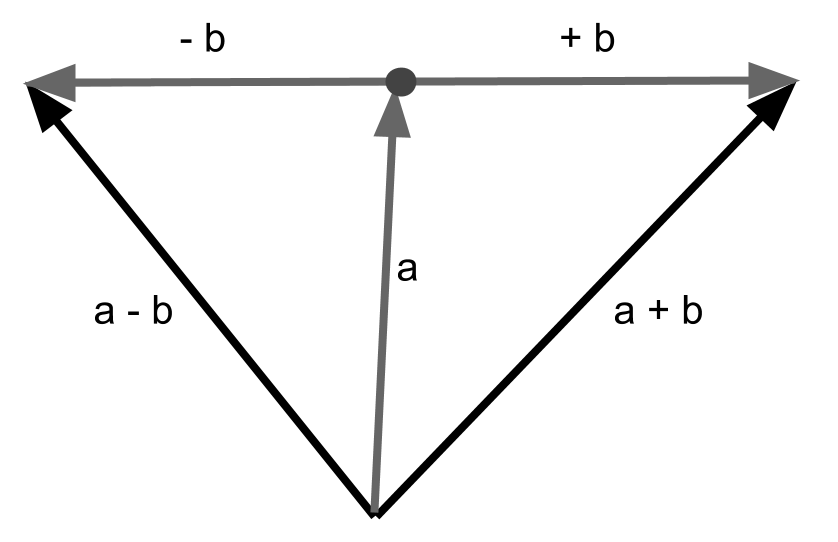
\includegraphics[scale=0.2]{Diagrams/vector_addition.png}
			\label{3DAxisFigure}
		}
		\caption{Table of common dot product tests between two vectors.}
	}
\end{figure}
\FloatBarrier

\noindent
A useful type of vector is known as a unit vector. This is a type of vector which has a magnitude of 1. Unit vectors are used extensively in computer graphics particularly with ragards to \gls{Shader}s. Take the vector v its magnitude $\alpha$ can be calculated by taking the square root of the product its components squared, as seen below 

\begin{equation}
	\alpha =~ \mid \textbf{v} \mid~ = \sqrt{\textbf{v}^2_x + \textbf{v}^2_y + \textbf{v}^2_z}
\end{equation}

The unit vector can then be calculated by taking the product of $v$ and the reciprocal of its magnitude shown in the following equation.

\begin{equation}
	\upsilon = \frac{\textbf{v}}{\alpha} = \frac{1}{\alpha} \textbf{v}
\end{equation}

There are many different ways to multiply vectors, however, in 3D graphics there two main multiplications. These being the dot and cross product. The dot product yields a scalar by adding the products of the vector product components. The cross product on the other hand is the product of two vectors which gives a vector which is perpendicular. The dot product can be calculated using the formula below: 

\begin{equation}
a \cdot b = a_x b_x + a_y b_y + a_z b_z = d
\end{equation}

\noindent
Some of the main uses for dot products within 3D graphics is to find whether two vectors are collinear, perpendicular, in the same direction or opposite directions. One possible use for this is to find the dot product of two branches directions in order to find out if they growing in the same direct or in opposite directions. In the table \ref{dot product test} below, there are each of the dot product test diagrams as well as the test equation where $ab = \mid a \mid \mid b \mid = a \cdot b$.

\begin{table}[h!]
\centering
\begin{tabular}{ | c | c | c |}
\hline
	Test 	& Equation & Example\\  
\hline
\hline
	Collinear 							& $(a \cdot b) = ab$ & 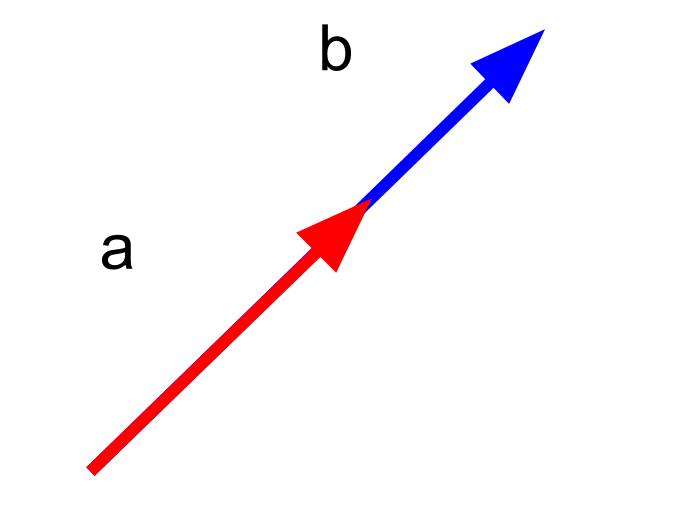
\includegraphics[scale=0.1]{Diagrams/vector1.png}\\
\hline
	Opposite Collinear 					& $(a \cdot b) = -ab$ &	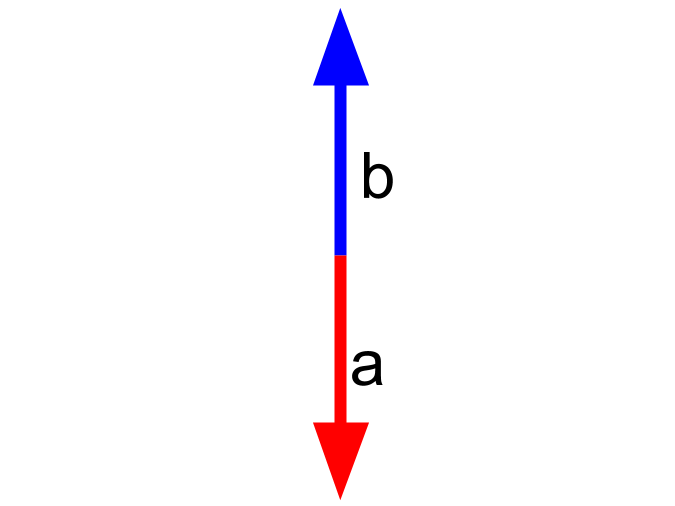
\includegraphics[scale=0.1]{Diagrams/vector2.png}\\
\hline
	Perpendicular 						& $(a \cdot b) = 0$	&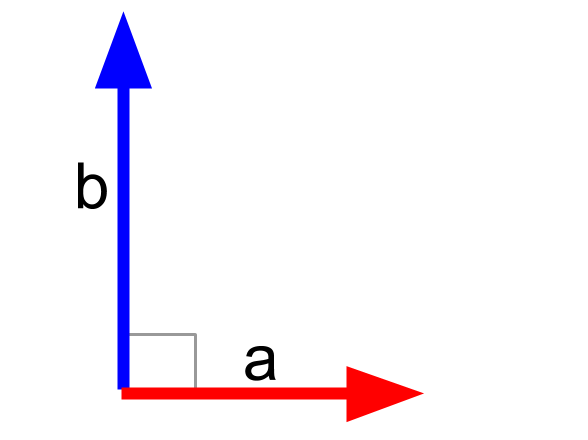
\includegraphics[scale=0.1]{Diagrams/vector3.png}\\
\hline
	Same Direction 						& $(a \cdot b) > 0$ &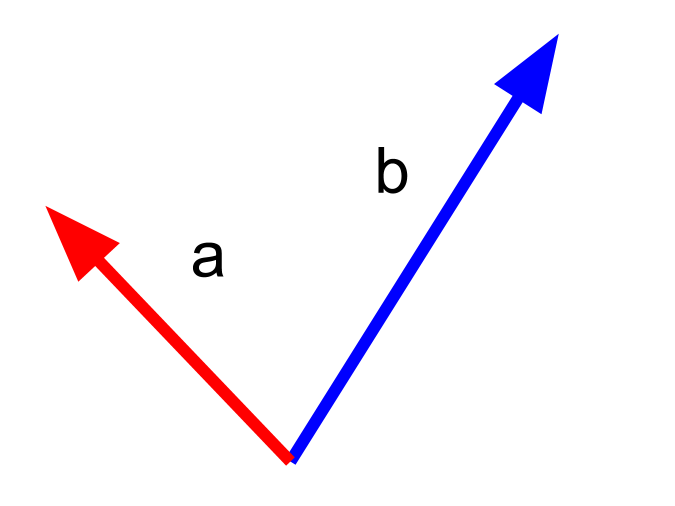
\includegraphics[scale=0.1]{Diagrams/vector4.png}\\
\hline
	Opposite Direction 					& $(a \cdot b) < 0$ &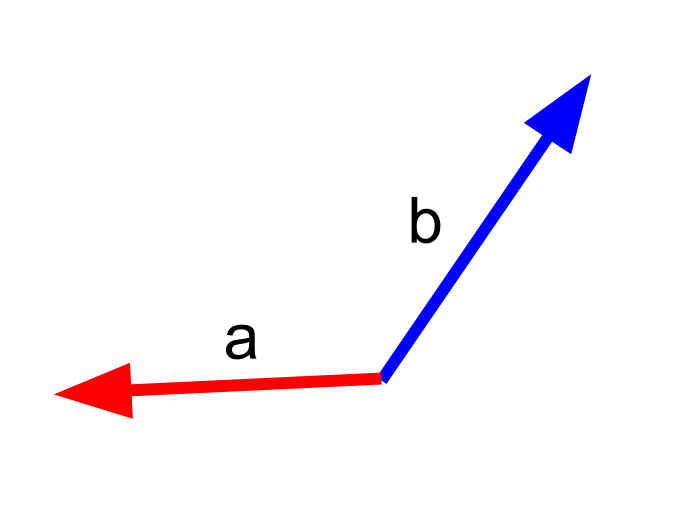
\includegraphics[scale=0.1]{Diagrams/vector5.png}\\
\hline

\end{tabular}
\caption{Table of turtle instruction symbols and their meaning to the interpreter}
\label{dot product test}
\end{table}
\FloatBarrier

\noindent
The cross product also known as the outer product takes two vectors and finds the perpendicular vector of the two vectors, this is only possible in 3D space and can be expressed in the following formula using the left-hand rule: 

\begin{equation}
a \times b = [(a_y b_z - a_z b_y), (a_z b_x - a_x b_z), (a_x b_y - a_y b_x)]
\end{equation}

\noindent
The result of a cross product can be seen in figure \ref{Cross product diagram} below. Where vectors $a$ and $b$ give the perpendicular vector $a \times b$. The cross product is very useful within physics calculations when it is necessary to find the rotational motion. 

\noindent
Some of the properties of the cross product are as follows:

\begin{itemize}
	\item is non-commutative, meaning order matters($a \times b \not= b \times a$).
	\item is anti-commutative ($a \times b = -(a \times b)$).
	\item is distributive with addition ($a \times (b + c) = (a \times b) + (a \times c)$).
\end{itemize}

\begin{figure}[htbp]
	{\centering
		\setlength{\fboxrule}{1pt}
		\vspace{7px}
		\fbox{
			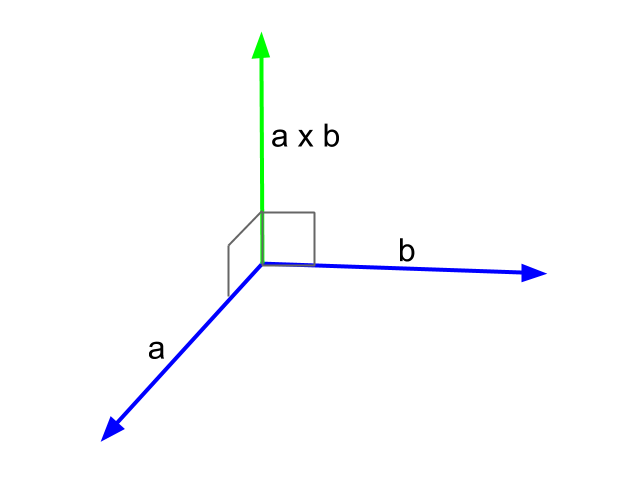
\includegraphics[scale=0.25]{Diagrams/cross_product.png}
			\label{Cross product diagram}
		}
		\caption{Diagram of the cross product of two vectors a and b.}
	}
\end{figure}
\FloatBarrier

\subsection{Matrices}

A model in 3D space will exist as a set of vertices which each have a position. Moving the model requires moving all of the the vertices of that model without distorting it in any way, this is called a model transform. There are four main types of transforms; translation, rotation, scale and shear. Matrices are a single matematical construct which is capable of carrying out all four of these transformations. This sections will only cover the first three as the shear transformation is likely not going to be useful for this thesis.    

A matrix is an 2D array of numbers, arranged into rows and columns, which can come in many different sizes. In 3D graphics, matrices used for transformations are the 3 $\times$ 3 and 4 $\times$ 4 matrix as seen below. A 3 $\times$ 3 matrix can be used for linear transorms such as scaling and rotation, furthermore, a linear transform which contains translation is known as an affine transform and can be represented by a 4 $\times$ 4 matrix known as an Atomic Transform Matrix. An atomic Transfom matrix is the concatination of four 4 $\times$ 4 matrices, one for translations, rotations, scale and shear transforms. Resulting in a 4 $\times$ 4 matrix as shown below. 

\begin{equation}
\textbf{M} = \begin{bmatrix}
M_{11} & M_{12} & M_{13} \\
M_{21} & M_{22} & M_{23} \\
M_{31} & M_{32} & M_{33}
\end{bmatrix}
\end{equation}

\begin{equation}
\textbf{M} = \begin{bmatrix}
M_{11} & M_{12} & M_{13} & M_{14}\\
M_{21} & M_{22} & M_{23} & M_{24}\\
M_{31} & M_{32} & M_{33} & M_{34}\\
M_{41} & M_{42} & M_{43} & M_{44}
\end{bmatrix}
\end{equation}

\noindent
The affine matrix can be shown in the expression below where $RS$ is a 3 $\times$ 3 matrix containing the rotation and scale where the $4^th$ elements are 0. The $T$ elements represent the translation with the 4th element being 1. 

\begin{equation}
\textbf{M} = \begin{bmatrix}
RS_{11} & RS_{12} & RS_{13} & 0\\
RS_{21} & RS_{22} & RS_{23} & 0\\
RS_{31} & RS_{32} & RS_{33} & 0\\
T_{1} & T_{2} & T_{3} & 1
\end{bmatrix}
\end{equation}

The product of two linear transform matrices will be another linear transform matrix that carries out both of those tranformations. This is true for the multiplication of two affine transform matrices as well, and is why matrix multiplication is so powerful in 3D graphics. Take the two matrices $A$ and $B$ which give the product $P$. In order to multiply $A$ and $B$ together, the dot product of the row and the column is calculated as seen below. It is also imporant to know that matrix multiplication is non-commutative $(AB \not= BA)$.

\begin{equation}
\textbf{AB} = \begin{bmatrix}
A_{11} & A_{12} & A_{13}\\
A_{21} & A_{22} & A_{23}\\
A_{31} & A_{32} & A_{33}
\end{bmatrix}
\times
\begin{bmatrix}
B_{11} & B_{12} & B_{13}\\
B_{21} & B_{22} & B_{23}\\
B_{31} & B_{32} & B_{33}
\end{bmatrix}
= \begin{bmatrix}
(A_{row1} \cdot B_{col1}) & (A_{row1} \cdot B_{col2}) & (A_{row1} \cdot B_{col3})\\
(A_{row2} \cdot B_{col1}) & (A_{row2} \cdot B_{col2}) & (A_{row2} \cdot B_{col3})\\
(A_{row3} \cdot B_{col1}) & (A_{row3} \cdot B_{col2}) & (A_{row3} \cdot B_{col3})
\end{bmatrix}
\end{equation}

To translate a vertex in 3D space without causing any distortion. The vertex can be added the the matrix below as follows. These translations can be carried out on all vertices in order to translate a whole object model. 

\begin{equation}
V + T = \begin{bmatrix}
V_{x} \\
V_{y} \\
V_{z}~ \\
1
\end{bmatrix}
+
\begin{bmatrix}
1 & 0 & 0 & 0\\
0 & 1 & 0 & 0\\
0 & 0 & 1 & 0\\
T_{x} & T_{y} & T_{z} & 1
\end{bmatrix}
= \begin{bmatrix}
(V_x + T_x)~ \\
(V_y + T_y)~ \\
(V_z + T_z)~ \\
1
\end{bmatrix}
\end{equation}

\noindent

In order to rotate a vertex in 3D space the vertex position and the rotation angle can be applied to the as a matrix depending on the axis about which it is rotating. These rotation matrices can be applied to the vertex itself in order to gain the new position of the vertex. 

\begin{equation}
R_x(\theta) = 
\begin{bmatrix}
(v_x)~ \\
(v_y)~ \\ 
(v_z)~ \\
1
\end{bmatrix}
\begin{bmatrix}
1 	& 0 					& 0 					& 0\\
0 	& \text{cos}(\theta) 	& \text{sin}(\theta) 	& 0\\
0 	& -\text{sin}(\theta) 	& \text{cos}(\theta) 	& 0\\
0 	& 0 					& 0 					& 1
\end{bmatrix}
\end{equation}

\begin{equation}
R_y(\theta) = 
\begin{bmatrix}
(v_x)~ \\
(v_y)~ \\
(v_z)~ \\
1
\end{bmatrix}
\begin{bmatrix}
\text{cos}(\theta) 	& 0 					& -\text{sin}(\theta) 	& 0\\
0 					& 1						& 0						& 0\\
\text{sin}(\theta) 	& 0 					& \text{cos}(\theta)	& 0\\
0 					& 0 					& 0 					& 1
\end{bmatrix}
\end{equation}

\begin{equation}
R_z(\theta) = 
\begin{bmatrix}
(v_x)~ \\
(v_y)~ \\
(v_z)~ \\
1
\end{bmatrix}
\begin{bmatrix}
\text{cos}(\theta) 	& \text{sin}(\theta) 	& 0						& 0\\
-\text{sin}(\theta) & \text{cos}(\theta) 	& 0
					& 0\\
0 					& 0 					& 1						& 0\\
0 					& 0 					& 0 					& 1
\end{bmatrix}
\end{equation}


\begin{equation}
ST = \begin{bmatrix}
S_{x} \\
S_{y} \\
S_{z} \\
1
\end{bmatrix}
\begin{bmatrix}
S_x & 0 & 0 & 0\\
0 & S_y & 0 & 0\\
0 & 0 & S_z & 0\\
0  & 0  & 0 & 1
\end{bmatrix}
= \begin{bmatrix}
(S_x R_x)~ \\
(S_y R_y)~ \\
(S_z R_z)~ \\
1
\end{bmatrix}
\end{equation}

\subsection{Quaternions}

In computer graphics there are a number of ways to represent 3D rotations. One method is to use matrices, as spoken about in the previous section. Matrices are often used to represent rotation, however, it has a number of limitations. Matrices are represented by nine floating point values and can be computationally expensive store and, process particularly when doing a vector to matrix multiplication. There are also situations where it is neccessary to smoothly transition from one rotation to another, or find a certain degree of rotation between two rotations. For example, when calculating the rotation of branch segments between time intervals in physics calculations. It is possible to make these calculations using matrices but it can become very complicated and even more computationally expensive. Quaterions are the miraculous answer to all of these difficulties.\\

Quaternions look similar to a 4D vector, as contains 4 axes $q = [qx, qy, qz, qw]$, these are represented with a real axis ($qw$) and three imaginary axis $qx, qy, qz$. A quaternion can be represented in complex form as follows: 

\begin{equation}
q = (iq_x + jq_y + kq_z + qw)
\end{equation}

For the purpose of this thesis it is not important to understand the derivation of quaterions in mathematics, however it is important to understand that any unit length quaternion which obays the rule in \ref{unit quat} below. 

\begin{equation} \label{unit quat}
	q_x^2 + q_y^2 + q_z^2 + q_w^2 = 1
\end{equation}

\noindent
Unit quaternions are used for rotations, it is possible to convert a quaternion to a unit quaternion  by taking the angle and the axis of a rotation and applying to the quaternion as follows: 

\begin{equation}
\begin{aligned}
& q = [qx, qy, qz]\\
& \text{where} \\
& q_x = a_x sin \frac{\theta}{2}\\
& q_y = a_y sin \frac{\theta}{2}\\
& q_z = a_z sin \frac{\theta}{2}\\
& q_w = cos \frac{\theta}{2}
\end{aligned}
\end{equation}

\noindent
The scalar part $q_w$ is the cosine of the half angle, and the vector part $q_x q_y q_z$ is the axis of that rotation, scaled by sine of the half angle of rotation. The unit quaternion can be used for rotations in a number of ways. The most useful of which is to rotate vectors, concatonate rotations together similar to how matrix transformations can be multiplied together as well as interpolate between two rotations. \\

The first operation for quaternions is that of addition. Simply the addition of two quaternions is just the component wise addition of the two quaternions, similar to that of matrices addition.

\begin{equation}
p + q = [(p_w + q_w), (p_x + q_x), (p_y + q_y), (p_z + q_z)]
\end{equation}

There are a number of types of quaternion multiplication, however, the one most commonly used for quaternion rotaton is called the grassmann product. This can be described in the following formula below. Where $p$ and $q$ are quaternions and the subscript $w$ indicates the scalar part and subscript $x, y, z$ indicate the vector components of each quaternion.

\begin{equation}
\begin{aligned}
R = r_w + r_x + r_y + r_z\\
\text{where}\\
r_w = p_w q_w - (p_x q_x + p_y q_y + p_z q_z)\\
r_x = p_w q_x + p_x q_w + p_y q_z - p_z q_y\\
r_y = p_w q_y + p_y q_w - p_x q_z + p_z q_x\\
r_z = p_w q_z + p_z q_w + p_x q_y - p_y q_x\\
\end{aligned}
\end{equation}

To rotate a vector by a unit quaternion the vector will need to be converted into its quaternion form. This requires taking the unit vector $v$ and using it as the vector part of the quaternion with a scalar part being equal to zero. This can be written as $Q_v = [v, 0] = [v_x, v_y, v_z, 0]$. In order to rotate the vector we can therefore take the grassmann product of the rotation quaternion $q$ and the vector form quaternion $v$ and the inverse of the rotation quaternion $q^-1$. \\

\begin{equation}
	V_q = qvq^{-1}
\end{equation}

\noindent
For unit quaternions the conjugate and the inverse are identical. The inverse of a unit quaternion can be calculated as follows. 

\begin{equation}
	q^{-1} = [-q_v, q_s]
\end{equation}

\noindent
Quaternion rotations can be concatonated together similar to how matrix transforms can be multiplied together. The order by which rotations matter but using the grassmann product the rotations can easily be multiplied together to give the result of all of those rotations as if they were to happen one after the other. This can be expressed as follows:

\begin{equation}
\begin{aligned}
Q_{net} = Q_3 Q_2 Q_1\\
v' = Q_3 Q_2 Q_1~ v~ Q_{1}^{-1} Q_{2}^{-1} Q_{3}^{-1}
\end{aligned}
\end{equation}

\noindent
The order in which the quaternions $Q_1, Q_2$ and $Q_3$ are applied is in the order $Q_3~$ then $Q_2~$ and then $Q_1$. To apply this to a vector the product of the three quaternions is multiplied to the vector and then multiplied to the product of the inverse of each quaternion. \\ 


\section{Model Generator}

Modeling the branches of a plant is one of the most important parts for the overall look and feel of that plant that is being generated. The L-system described in the previous sections is able to describe the details about the plants structure, for instance the position, width, length, weight and other important information. The job of the model generator is to take this information and intelligently generate the models vertices, normals, texture coordinates and other information that can then be provided to the OpenGL renderer and finally to the GPU to be rendered on the screen.

The simplest way to generate a model for a branching structure of a plant would be to take a number of cylinders, and to rotate and stack them according to each joints position in 3D space. The up side to this approach is that every branch within the plant shares the same object model, depending on the position, rotation and scale of the branch the relavent matrix transforms can be applied. In this way we are able to represent the overall branching structure of the plant. However, there is a problem which is pointed out by Baele and Warz\'{e}e "The branches junction causes a continuity problem: to simply stack up cylinders generates a gap" \cite{baele2005real}. This can be shown in the figure below:

\FloatBarrier

\begin{figure}[htbp]
	{\centering
		\vspace{7px}
		\setlength{\fboxrule}{1pt}
		\fbox{
			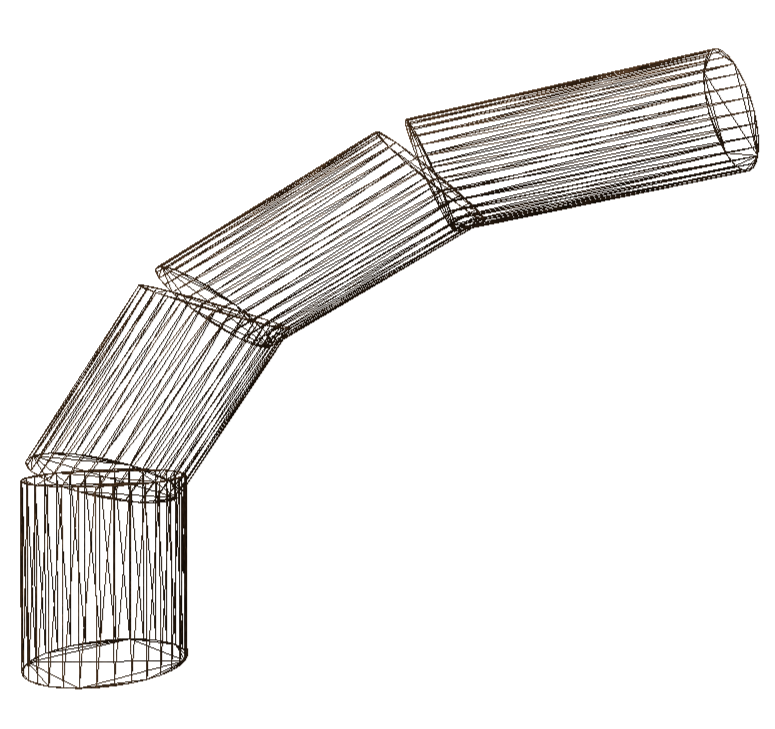
\includegraphics[scale=0.2]{Diagrams/stackedBranchesMesh.png}
		}
		\caption{Example of the continuity problem faced with stacked branching with a 25$^{\circ}$ bend per joint.}
	}
\end{figure}

\FloatBarrier

\noindent
This simple method of stacking cylinders gives a reasonable looking tree structure and it is usually good enough when the angles of branches are not more than 25$^{\circ}$ and the size of the branches do not change. However for a much more convincing tree structure there will need to be a better solution. The logical next step would be to actively link the branch segments together. This requires a number of things to take place, first of all the vertices from the previous branch top must be linked with the new top of the branch. These are the circles of vertices at either end of each branch segment. These circles will have to rotate depending on the bending direction of the branch. This means that the final model will not be made up of a large number of the same model but rather a single model with many linked branches. An example of this can be seen below:

\begin{figure}[htbp]
	{\centering
		\vspace{7px}
		\setlength{\fboxrule}{1pt}
		\fbox{
			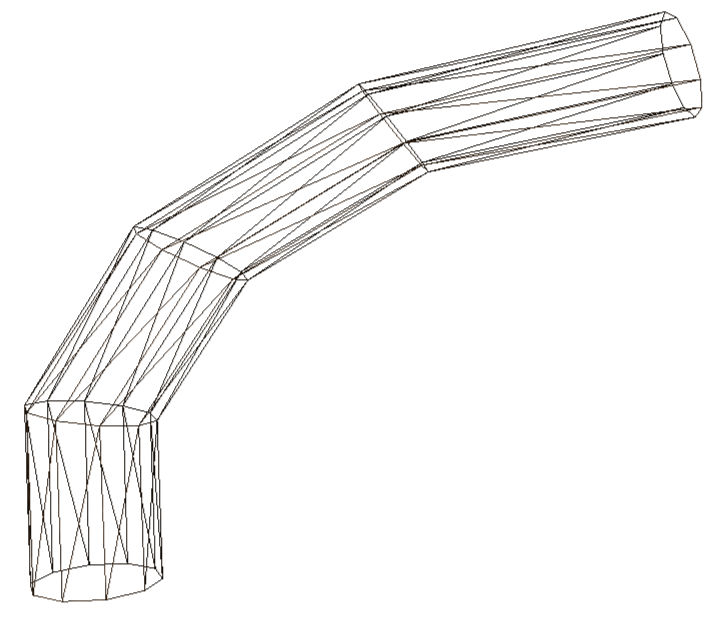
\includegraphics[scale=0.2]{Diagrams/linkedBranchesMesh.png}
		}
		\caption{Example of linked branching with a 25$^{\circ}$ bend per joint.}
	}
\end{figure}
\FloatBarrier

\noindent
This method of branch generation gives a very similar result at first glance to that of stacking cylinders. Although it does have a number of advantages, firstly it completely avoids the branch gap problem that happens with angle changes as well as branch size changes. It also means that the resolution is dynamic, meaning the number of vertices that make up a cylinder can be dynamically changed. This means that a very high resolution tree can be rendered which may look very smooth but will take a lot more computational resources, or a very low resolution tree can be rendered with more jagged edges but will require a lot less computational resources. This can be seen in figure \ref{} below, where similar a looking branch can be acheived using less than half the number of vertices, with joined branches instead of stacked branches.

\begin{figure}[htbp]
	{\centering
		\vspace{7px}
		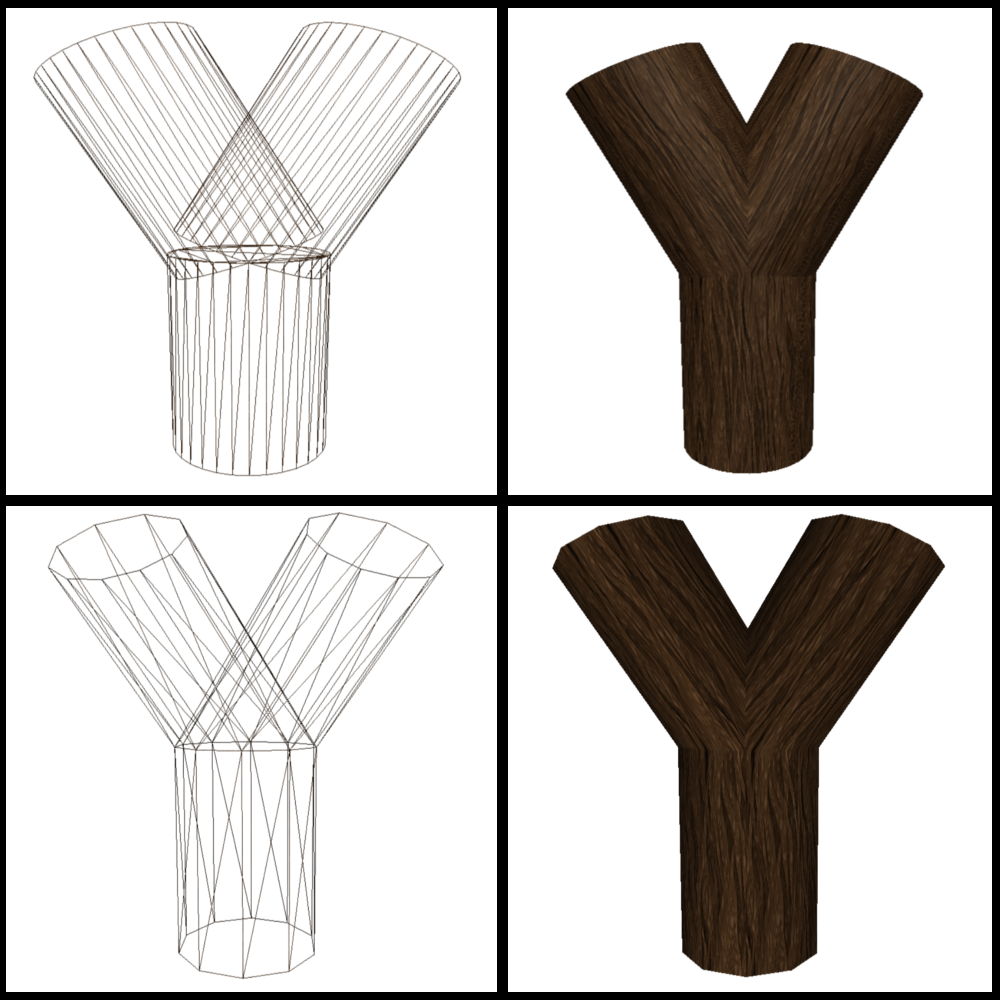
\includegraphics[scale=0.2]{Diagrams/StackedVsLinked.png}
		\caption{Stacked Vs Linked.}
	}
\end{figure}
\FloatBarrier



\section{Renderer}

\noindent
The renderer is the final stage in the procedural generation pipeline. It takes all of the 3D models generated by the model generator, such as leaves, branches and flowers and renders them on the screen.  For this thesis, the \acrlong{opengl} (\acrshort{opengl}) application programming interface is use used to efficiently render the models on the screen using the \acrlong{gpu} (\acrshort{gpu}). 

The \acrshort{gpu} is a specially designed piece of harware for processing computer graphics and image processing, it has hundereds of individual compute cores which can be used in parallel. Due to the highly parallel nature of the \acrshort{gpu}, the \acrshort{opengl} framework helps to abstract the hardware and create an interface to interact with the \acrshort{gpu} in a simpler way. There are a number of other types of graphics \acrshort{api} such as Vulkan, Metal or DirectX. These \acrshort{api}s all provide a way of interacting with the hardware behind the scenes, However, they each have a different approach. Therefore, this section will not be be going into great detail about about the specifics of \acrshort{opengl} but rather the general concepts required for rendering the plant model on the screen.

\subsection{Models and Buffer Objects}

The model generator produces all of the information neccessary for the renderer to produce the result on the screen. In general the model data will consist of vertex data, texture co-ordinates and vertex normals. The vertex data is simply position of a point within a model, three vertices make up a face and the faces are what are ultimately rendered on the screen. The texture co-ordinates are the locations on a texture image which maps directly to the model vertices. Finally the vertex normals simply known as normals are the average normal vector. A normal vector being the vector that is purpendicular to the surface at a given point, and can be used for Phong shading or other types of lighting techniques.  

One of the most important parts of the rendering process is buffering the model data onto the \acrshort{gpu}. The \acrlong{vbo} (\acrshort{vbo}) is a data structure within the \acrshort{opengl} library which can be used to store this data on the \acrshort{gpu}. Generally, the data is stored as a single buffer or array with the first 3 values being a vertex position, the second two being a texture co-ordinate and the last three being a vertex normal. 

\begin{figure}[htbp]
	{\centering
		\vspace{7px}
		\setlength{\fboxrule}{1pt}
		\fbox{
			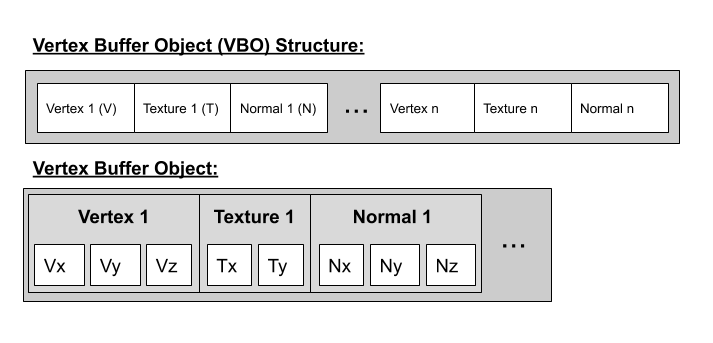
\includegraphics[scale=0.5]{Diagrams/VertexObjects.png}
		}
		\caption{Diagram showing the structure of a vertex buffer object.}
	}
\end{figure}
\FloatBarrier

 










\chapter{Physics Simulator} \label{physics chapter}
\lettrine[lines=3]{P}{}hysics simulations are becoming more common in many types of 3D graphics applications, particularly in video games. Physics engines such as Bullet, PhysX, Havok, and others are used to simulate anything from projectiles to ragdoll physics. These are known as physics engines because they are complex systems for simulating many common types of simulations. Simulating plant-life using a physics engine may be possible; however, these types of systems are continually being updated and changed. In order to keep this information relevant, this thesis will implement a full physics simulator to simulate plants generated by the L-system. Using a physics engine instead of the purpose-built simulator should be relatively straightforward, as the L-system generates a tree skeleton with all of the joint information such as width and length. Any other information that is needed can be provided through module parameters in the L-system and added to the joint information. Currently, the joint contains the following information: branch length, branch width, weight, spring constant, damping constant, momentum, as well as its rotation and position. 

This chapter will discuss a purpose-built method of simulating the physical motion of plant-life, laid out by Barron et al. \cite{barron2001real}. This method will be built so that it interacts with the L-system itself in such a way that the L-system can provide the parameters necessary for the simulation. This will allow a physics simulation to be run on any plant generated by the L-system.  

The primary technique discussed by Barron et al. for simulating the motion of a system like a tree or a plant, is taken from that of a particle system, first described by Reeves \cite{reeves1983particle}. Particle systems can be applied to simulate phenomena like clouds, smoke, water, and fire. The main advantage of particle systems is that the motion for each particle can be updated simultaneously. This technique can be applied to the L-system representation of plant-life, where branches are split into segments that make up a skeleton of segments or joints. Each joint can represent a \say{particle} within the system, which has a dependency on all of its parent branches.

The particle system concept can be used to simulate the motion of the plant by having each joint within the plant skeleton provide some basic physical properties. These properties include but are not limited to the width, length, direction vector, spring consistent, and dampening constant. The direction vector is the global direction that the branch is pointing in 3D space. The spring constant and the dampening constant are used in Hooke's Law calculations. The spring force of the branch resists it from bending. Whereas gravity, wind, and other forces generate torque, which generally acts against this spring force, causing the branch to bend.

\begin{figure}[htbp]
	{\centering
		\vspace{7px}
		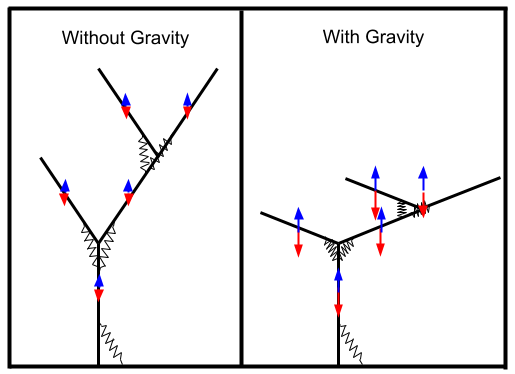
\includegraphics[scale=0.5]{Diagrams/HookesLaw.png}
		\caption{Diagram showing how Hooke's Law can be applied to a plant structure.} \label{rewriter diagram}
	}
\end{figure}
\FloatBarrier

\noindent
This chapter defines a method of calculating the physical motion of a plant, where the properties can be defined in an L-system. The chapter starts by explaining how the volume, mass, inertia, and displacement of a given branch can be calculated. It then moves on to explain Hooke's Law and its role within the simulation of plant movement. The equations of motion in a 3D setting are then explained. Finally, this chapter talks about the challenges faced with efficiency when updating branches and some of the results that can be achieved by using this method. 

\section{Physical Properties of Branches}

The mass of each branch segment can be simply calculated by taking the volume of each branch and multiplying it by the density of the wood or material. To do this the volume of each branch needs to be calculated. This can be done by multiplying $\pi$ by the radius $r$ squared and the length $l$ as sees below.

\begin{equation}
v  = \pi r^2 l
\end{equation}

\noindent
The volume of the branch segment is not often a clean cylindrical shape, particularly if the branch segment is decreasing in size. However, it gives a good indication as to the volume of the branch. The volume can now be used to calculate the mass. Calculating the mass also requires the density of the material. For instance the density of pine wood is between 400 - 420 $\text{kg/m}^3$. Some woods being less dense at about 200 $\text{kg/m}^3$, and other hardwood being as dense as 1000$\text{kg/m}^3$. The denser the wood, the higher the mass, and ultimately the greater its resistance to its change in velocity.

\begin{equation}
m = v \times d
\end{equation}

\noindent
The mass can be used to calculate each branch segments' moment of inertia. The moment of inertia is the branches' resistance to angular momentum. As the object is 3D, the shape of the object needs to be taken into account. Each branch can be seen as a long cylinder, which can be expressed in the following equation.

\begin{equation}
I = \frac{1}{3} m l ^ 2
\end{equation}

\noindent
Where $I$ is the inertia of the branch, $m$ is the mass, and $l$ is the length. Similarly, an inertia tensor can be used for the sake of convenience to describe better the objects' rotational inertia, which is used within vector and matrix calculations. The inertia will be used when calculating the velocity of each segment in section \ref{motion equations}. Below is an inertia tensor for a shape that is similar to that of a branch segment.


\begin{equation}
\begin{aligned}
I = \begin{bmatrix}
\frac{1}{12}m(3r^2 + l^2) 	& 0 							& 0 \\
0 							& \frac{1}{12}m(3r^2 + l^2)		& 0 \\
0 							& 0 							& \frac{1}{2}mr^2 
\end{bmatrix}
\end{aligned}
\end{equation}

\noindent
The next vital piece of information needed is the direction that torque is acting on the branch ($V$), depending on the forces that are acting on it. The vector that represents the direction that the branch is pointing is known as the forward vector ($v$). The torque can be calculated by taking the cross product of the forward vector $v$ and the force vector $w$. This can be visualised using the right-hand rule, where the index finger is the forward vector, and the middle finger is the force vector. The direction of the thumb then points in the direction of the torque. The angular velocity is produced as spin in the direction around the torque vector.

\begin{equation}
V = v \otimes w
\end{equation}

\noindent
The displacement is the change of angle of a branch from its resting position and is used to calculate the spring force of the branch in Hooke's Law. The displacement can be calculated by keeping track of the starting local resting rotation of the branch $p$ as well as its current rotation $q$ in the form of two quaternions. The difference quaternion $d$ is calculated by taking the local resting rotation $p$ and multiplying it by the inverse of its current rotation $q$. 

\begin{equation}
d = p \times q^{-1}
\end{equation}

\section{Hooke's Law} \label{hookes law}

Hooke's law is a law of physics that states that the resultant force from compressing or extending a spring is equal to the product of the spring constant and the displacement of the spring. Each branch in a plant structure can be seen as a type of semi-rigid spring where external forces like gravity or wind bend the spring. Hooke's law is used to calculate the reaction force due to the displacement of the spring. Hooke's Law can be expressed in the equation below.

\begin{equation}
f = -k _s d + k _d v
\end{equation}

\noindent
Where $f$ is the force exerted by the spring, $k _s$ is the spring constant, and $d$ is the total displacement of the spring. The dampening force can be calculated as $k _d v$ part where $k _d$ is the dampening constant, and $v$ is the velocity at the end of the spring or branch.


\section{Equations of Motion} \label{motion equations}

All of the forces such as gravity, wind, and spring forces can then be multiplied together to get the net force $f_{net}$ acting on the spring. This is used to calculate the momentum of the branch, where $T_{delta}$ is the change in time between physics calculations.

\begin{equation}
M = M_0 + f_{net} * T_{delta}
\end{equation}

\noindent
The velocity $v$ is the current speed of the branch. In 3D graphics, the velocity is represented as a 3D vector and can be calculated by taking the inverse of the inertia tensor $I$ and multiplying that by the momentum vector $M$.

\begin{equation}
v = I^{-1} * M
Q_v = [0, v]
\end{equation}

\noindent
The velocity vector can be converted to its quaternion form $Q_v$ in order to make the last step simpler. The scalar part of a quaternion can be set to 0, and the vector part can be set to $v$. This allows the next rotation quaternion $R$ to be calculated. The last part involves taking the previous rotation quaternion, the velocity of the branch, and the change in time, to calculate the next quaternion rotation of the branch.

\begin{equation}
R = R_0 + (\frac{1}{2} * Q_v * R_0 * T_{delta})
\end{equation}

\noindent
$R$ is the next local rotation quaternion, $R_0$ is the previous local rotation quaternion, $Q_v$ is the velocity quaternion, and finally, $T_{delta}$ is the change in time since the previous physics update. This new rotation quaternion can then replace the current local rotation of the branch, in turn, simulating the motion of the branch.

\section{Updating Branches}

The particles in this system are the joints within the trees' skeleton. All of the joints have to be updated in each update step. The updates can happen as frequently as needed. A consideration is that if the branches are not updated frequently enough, the animations will not look smooth. Effectively each update step needs to take the forces acting on each branch, its current position, and rotation and calculate the next position and rotation of that branch. This information is then used to generate the model of the tree once again. This position and rotation are passed to the renderer, which will render the result.

\newpage
\section{Summary}

This chapter outlined a method of simulating and animating a procedurally generated plant by representing each branch as a  particle in a larger particle system. The trees' skeleton provides information about the location, rotation, dimensions, and properties of each branch. The turtle graphics interpreter creates the skeleton during the interpretation stage. The properties of each branch can be simulated as a joint, which represents each particle within the entire tree system. Due to the embarrassingly parallel nature of particle systems, each branch update can be computed in parallel, either on the \acrshort{cpu} or \acrshort{gpu}. 

This physics system was purpose-built to demonstrate the concept behind the physics simulation; it might be possible or even beneficial in some cases to use an existing physics engine such as Bullet, PhysX, or Havok. The plant-skeleton and joints make it straightforward to use a physics engine if any additional physical parameters are required that information can be provided through the parameters of the l-system and stored in the joint information. 




\chapter{Results} \label{results chapter}
This thesis set out to design a software solution that uses the parametric L-system to representing complex plant-like structures and to explore whether the L-system can provide the relevant information necessary for physical simulation. This chapter will show several features of the parametric L-system, such as how varying parameters like branch width and branching angles can affect the resulting visual effect on the plant models. Furthermore, parameters that manipulate the physical behaviour of the plant under forces like wind or gravity are tested, and their results are discussed. All of the tests run in this chapter use the same interpreter and physics simulator, with the acceleration due to gravity at a constant value of $9.8m/s^2$. 

L-system \ref{parametric L-system results} defined below has several parameters that affect the look and behaviour of the resulting plant. The chosen parameters each have an effect on a visible property of plant when rendered or simulated.

The table below shows three sets of default values that will be applied to the L-system in each example. These parameters are numeric values and can be provided to the L-system by means of the \#define statements. Each test manipulates one or two of these parameters, and screenshots are taken to show the effects on the structure or how it reacts in the physical simulation. These features have the following meanings:


\begin{itemize}[noitemsep]
	\item n - The number of generations to rewrite
	\item a1 - The angle of the first pitch rotation in production rule 1
	\item a2 - The angle of the second pitch rotation in production rule 1
	\item a3 - The angle of both roll rotations in production rule 1
	\item dl - The proportion to increase the branch length each generation
	\item dr - The proportion to increase the branch width each generation
	\item scstart - The starting spring constant 
	\item scmod - The proportion to increase the spring constant each generation
\end{itemize}

\begin{singlespace}
\begin{equation}
\begin{aligned}
	&\textrm{\#object F BRANCH;}\\
	&\textrm{\#w : !(1.4)F(2.0, scstart)/(45)A(scstart);}\\
	&\textrm{\#p1 : A(sc) : * : !(dr)F(2, sc)[\&(a3)F(2, sc)A(sc)]/(a1)[\&(a3)F(2, sc)A(sc)]/(a2)[\&(a3)F(2, sc)A(sc)];}\\
	&\textrm{\#p2 : F(l, sc) : * : F(l*dl, sc*scmod);}\\
	&\textrm{\#p3 : !(w) : * : !(w*dr);}
\end{aligned}
\end{equation} \label{parametric L-system results}
\end{singlespace}

\vspace{10mm}
\hrule
\begin{table}[h!]
\centering
\begin{tabular}{ | c | c | c | c | c | c | c | c | c | }
\hline
	Variation Name & n & a1 & a2 & a3 & dl & dr & scstart & scmod\\  
\hline
\hline
	L-system 1  & 6 & 112.5 & 157.5 & 22.5 & 1.1 & 1.4 & 200 & 1.0 \\
\hline
	L-system 2  & 6 & 137.5 & 137.5 & 18.95 & 1.1 & 1.2 & 200 & 1.0 \\
\hline
	L-system 3  & 7 & 112.5 & 157.5 & 22.5 & 1.1 & 1.4 & 200 & 1.0 \\
\hline
\end{tabular}
\caption{Table of turtle graphics instructions symbols and their meaning to the interpreter}
\label{L-system params}
\end{table}
\FloatBarrier
\hrule

\vspace{10mm} 

\noindent
In the example in figure \ref{example thickness}, the value `dr', manipulates how thick each branch is. It does this during the rewriting process. Each time the width module `!' is encountered, it is rewritten with the current radius multiplied by the value of `dr', which increases the radius exponentially. This relationship can be expressed as $r_{i+1} = r_i \times dr$, where $r_i$ is the current branch radius and $r_{i+1}$ is the radius of the branch in the next generation. This relationship gives a tree that gets thicker exponentially as the branch moves closer to the base of the tree. These branch instructions will be rewritten a greater number of times at the base of the tree, compared to the top of three. This can be shown in the graphs in figure \ref{graph thickness} below. The relationship that determines the rate of change of the branch width can be cahnged. A tree that gets thicker linearly could have the relationship expressed as $r_{i+1} = r_i + dr$. In this case, each time a branch is rewritten, its size would grow by a constant amount, this would result in a tree that gets thicker much more progressively.

In the past example, the simulator is turned off, and therefore the tree is entirely static; however, the generated tree does have all the information required to be simulated. In fact, given the larger width of the branches near the base of the tree, they would have a higher mass and, therefore, more inertia, making them more resistant to changes in velocity. Due to this dependency between the branch width and the physical simulation, there will always be some correlation between the look of the tree and how it reacts to forces such as wind or gravity.

\begin{figure}[htbp]
	{\centering
		\vspace{7px}
		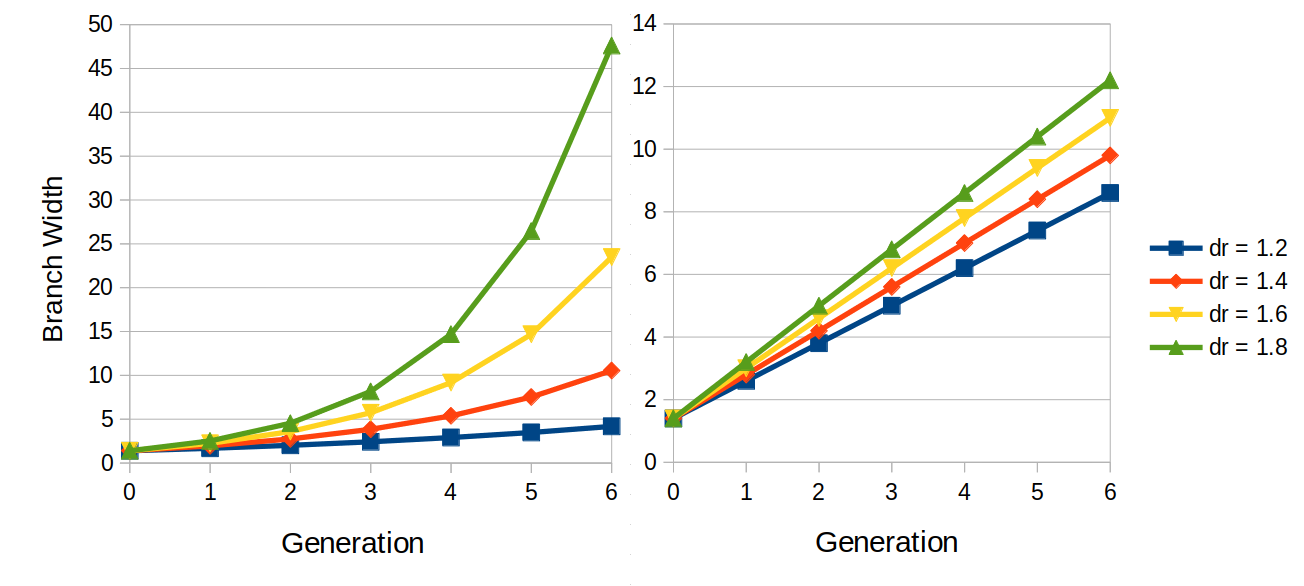
\includegraphics[scale=0.35]{Diagrams/branchWidthIncrease.png}
		\caption{Graph showing an exponential and linear relationship between the branch width and the generation when increasing the value of `dr'.} \label{graph thickness}
	}
\end{figure}
\FloatBarrier

\begin{figure}[htbp]
	{\centering
		\vspace{7px}
		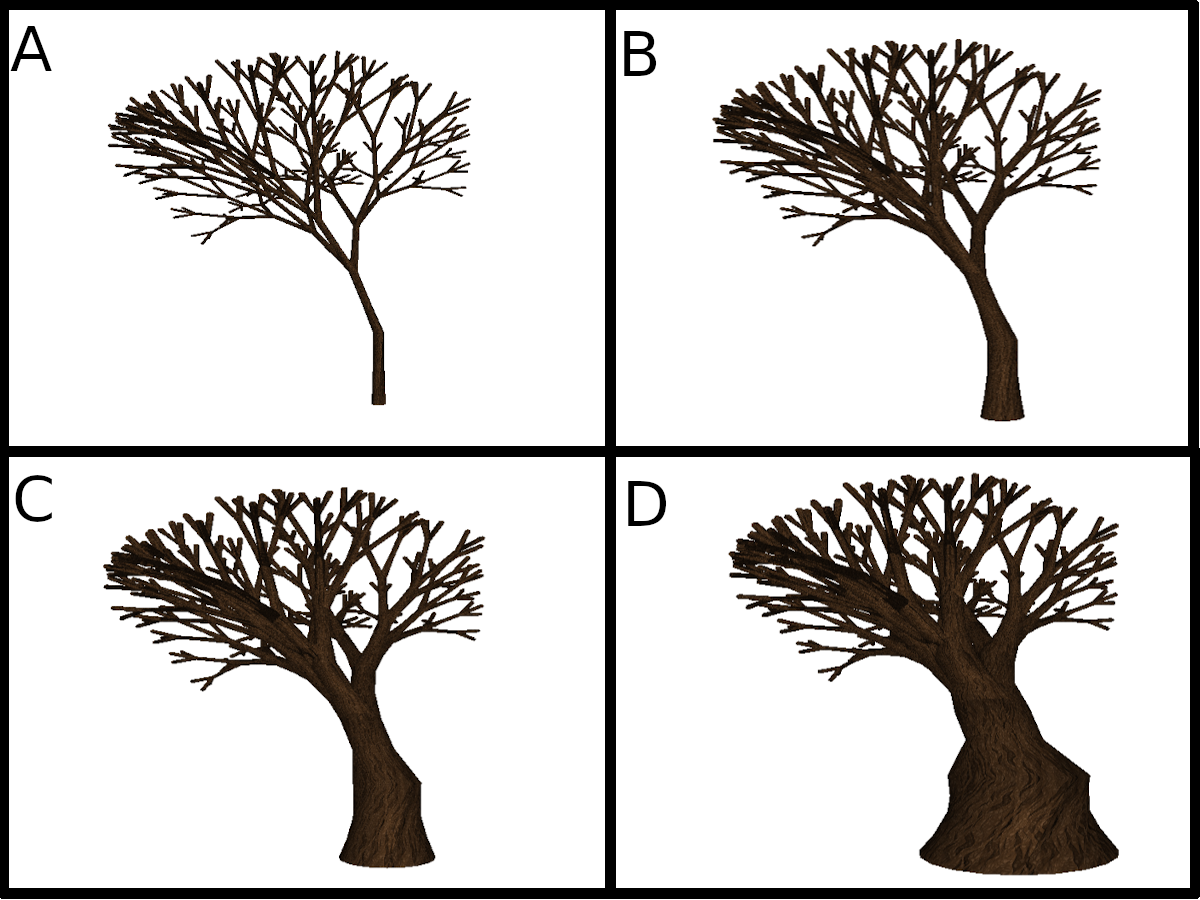
\includegraphics[scale=0.30]{Diagrams/TernaryBranching3_vr.png} 
		\caption{Examples of L-system 1 changing the `dr' variable which modifies the thickness of the base of the tree.} \label{example thickness}
	}
\end{figure}
\FloatBarrier

\noindent
Figure \ref{example angle} below shows that the result of changing the roll rotations' angle for some of the branches gives the tree a very different shape. In this case, increasing the angle of the branches' roll rotations from 15$^\circ$ to 30$^\circ$ can create a branch that curls slightly. Increasing this angle causes the result to be more dramatic. Furthermore, the angles of rotations can be randomised using the random range feature to have the same L-system produce many variations of the same structure. Manipulating the angles of rotations is a very powerful tool to allow very drastic changes to the look or behavior of a plant without changing its structure. 

\begin{figure}[htbp]
	{\centering
		\vspace{7px}
		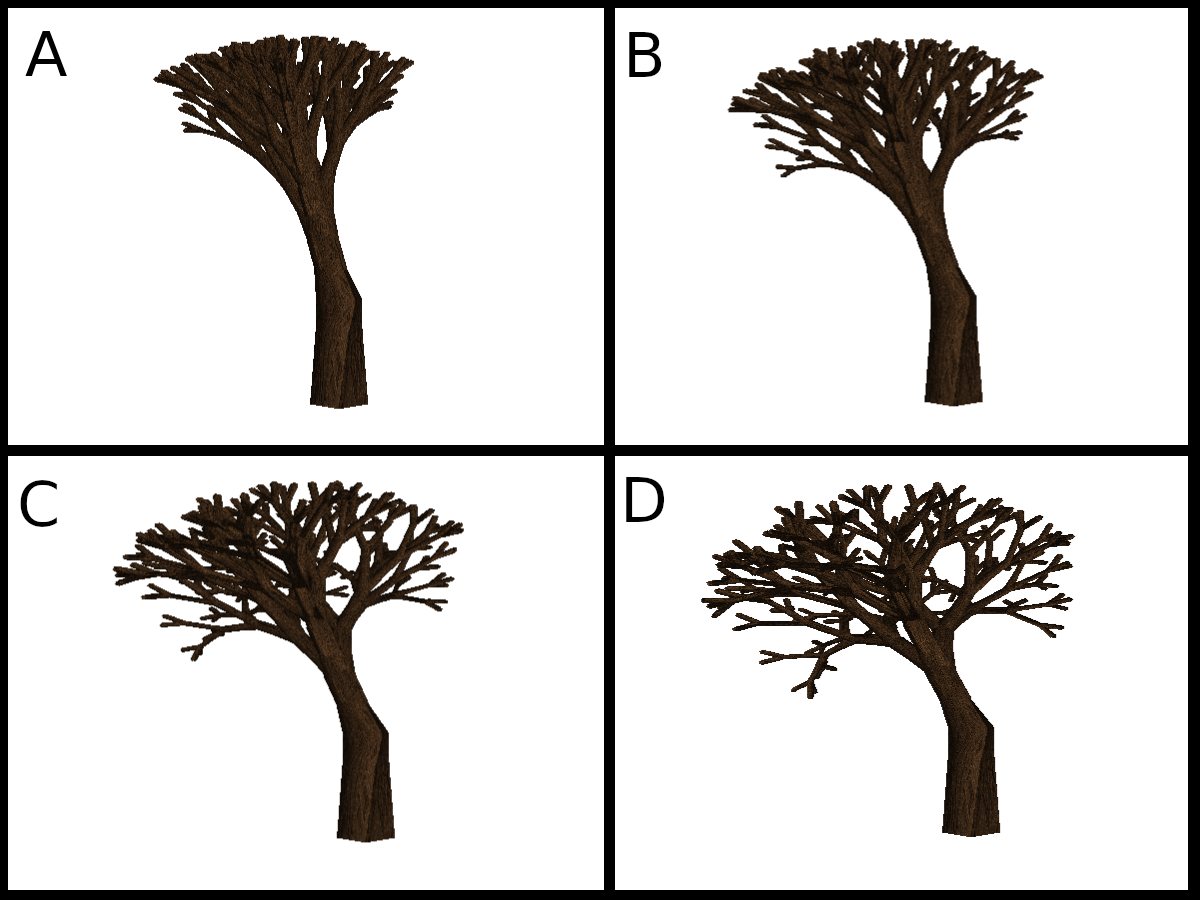
\includegraphics[scale=0.30]{Diagrams/TernaryBranching2_angle_example.png}
		\caption{Examples of L-system 2 changing the `a3' variable modifying the roll angle of certain branches.} \label{example angle}
	}
\end{figure}
\FloatBarrier

\noindent
If the angle is increased to 60$^\circ$ the result looks unrecognisable to its original structure. This can be seen in figure \ref{extreme example angle} below. The branch segment at the ends of the branch is rendered as a green sphere, this is to indicate where leaves may be rendered. It is easy to see how the functionality of these parameters can be advantagious, a user can create many variations of a tree without doing very much work, they only need to change a single parameters' value. 

\begin{figure}[htbp]
	{\centering
		\setlength{\fboxrule}{1pt}
		\vspace{7px}
		\fbox{
			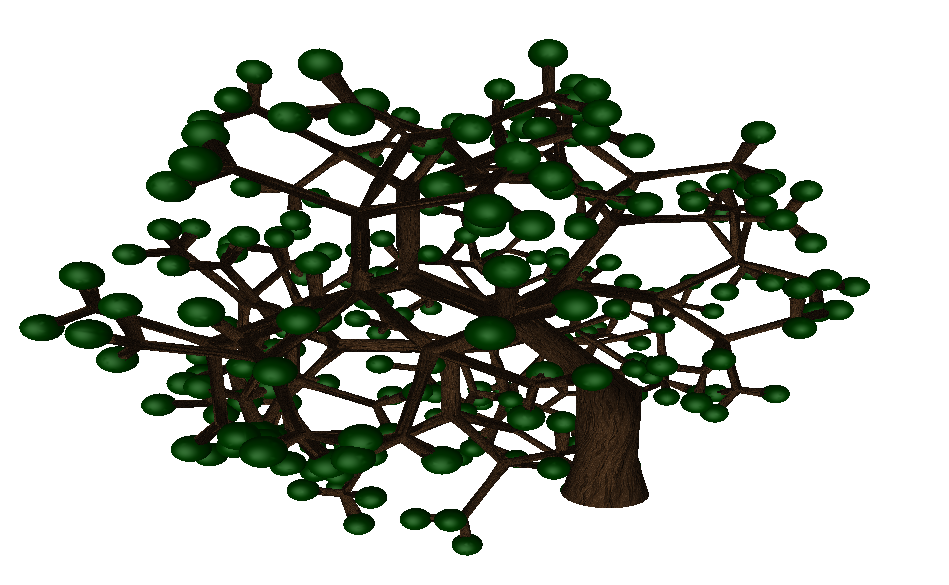
\includegraphics[scale=0.3]{Diagrams/ternarybranching3_a60.png}
		}
		\caption{L-system 2 where the variable `a3' has the value of 60$^\circ$. } \label{extreme example angle}
	}
\end{figure}
\FloatBarrier

\noindent
The previous tests have highlighted the capabilities of the parametric L-system without having the results be simulated. The advantage of having the simulator, interpreter, and rewriter as separate systems is the simulator and interpreter can choose to ignore specific parameters from the rewriter. For instance, if the L-system provides the physical properties of a plant, the simulator can easily be turned off, resulting in a static plant. Without running the simulator, the plant will become less resource-intensive to render, as it is not continuously updated. The next examples show that changing the physical properties of the plant can change how it responds when the simulator is turned on. Each screenshot where the plant is under gravity is taken after five seconds of the simulator running; this allows the branches' movement to settle into their final position.

As discussed in section \ref{hookes law}, discussing Hooke's Law, the spring constant is the In figure \ref{constant spring} below, the spring constant is a property of the spring which dictates the stiffness of the spring. In figure \ref{constant spring} `scstart' refers to the spring constant value when a branch is created. This is decreased from 200 to 50 at a decrement of 50. However, the spring constant modifier `scmod' is kept at 1.0; this value refers to the proportion to increase or decrease the spring constant by, in each generation. The spring constant for each branch is rewritten with the current spring constant multiplied by the spring constant modifier. This gives the relationship similar to how the width is calculated $sc_{i+1} = sc_i * scmod$. If the `scmod' value is 1.0, the spring constant will be a uniform value independent of how many generations there are. Leaving the spring constant the same throughout the tree assumes that thick branches at the base of the tree are as stiff as thin branches at the top of the tree. This is not accurate and will result in large branches bending unrealistically, particularly under extreme forces. Although this kind of behaviour would not be realistic, it highlights the flexibility of the system. If the physical properties are changed within the L-system, it will have a direct effect on the resulting model and simulation.

\begin{figure}[htbp]
	{\centering
		\vspace{7px}
		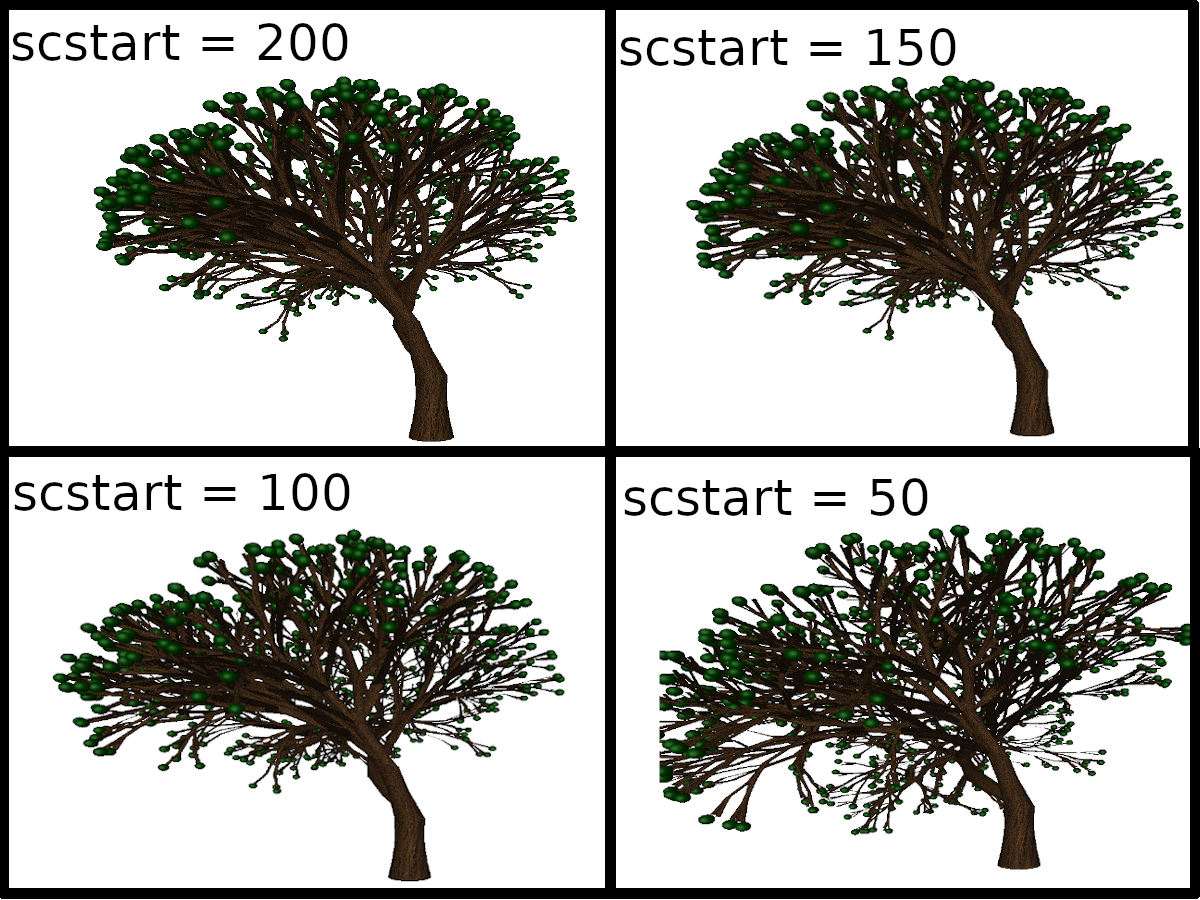
\includegraphics[scale=0.30]{Diagrams/TernaryBranching3_constantSC.png}
		\caption{Examples of L-system 1 when uniformly changing the `scstart' for all branches and leaving `scmod = 1.0'.}\label{constant spring}
	}
\end{figure}
\FloatBarrier

\noindent
The main limitation of the previous L-system example \ref{constant spring} is all the branches are the same stiffness. Creating more realistic simulation requires thinner branches to bend more than thicker ones. This can be achieved by using the spring constant modifier `scmod' value can be increased, resulting in the branches closer to the base being exponentially stiffer. Therefore, branches closer to the top are week and susceptible to smaller forces moving them around. As seen in figure \ref{increasing scmod} below, when the modifier is very high, the larger branches hardly bend at all, and the thinner branches only bend a small amount, whereas, with a lower modifier, the larger branches visibly bend and thinner bend a lot. The graphs in \ref{spring constant graphs} below, show a few different relationships of spring constant and spring constant modifiers and how they can be changed to produce different types of branch strengths during the rewriting process. The top right-hand graph is that used in figure \ref{constant spring}, where the spring constant modifier is 1.0, and only starting spring constant is changed. The top-left graph is used in figure \ref{increasing scmod}, where the modifier is decreased, but the starting spring constant is kept the same. Finally, the bottom graph shows how a modifier less than 1.0 could decrease the spring constant of branches the more they are rewritten; this would give the effect of branches near the base being less stiff than those near the top.

\begin{figure}[htbp]
	{\centering
		\vspace{7px}
		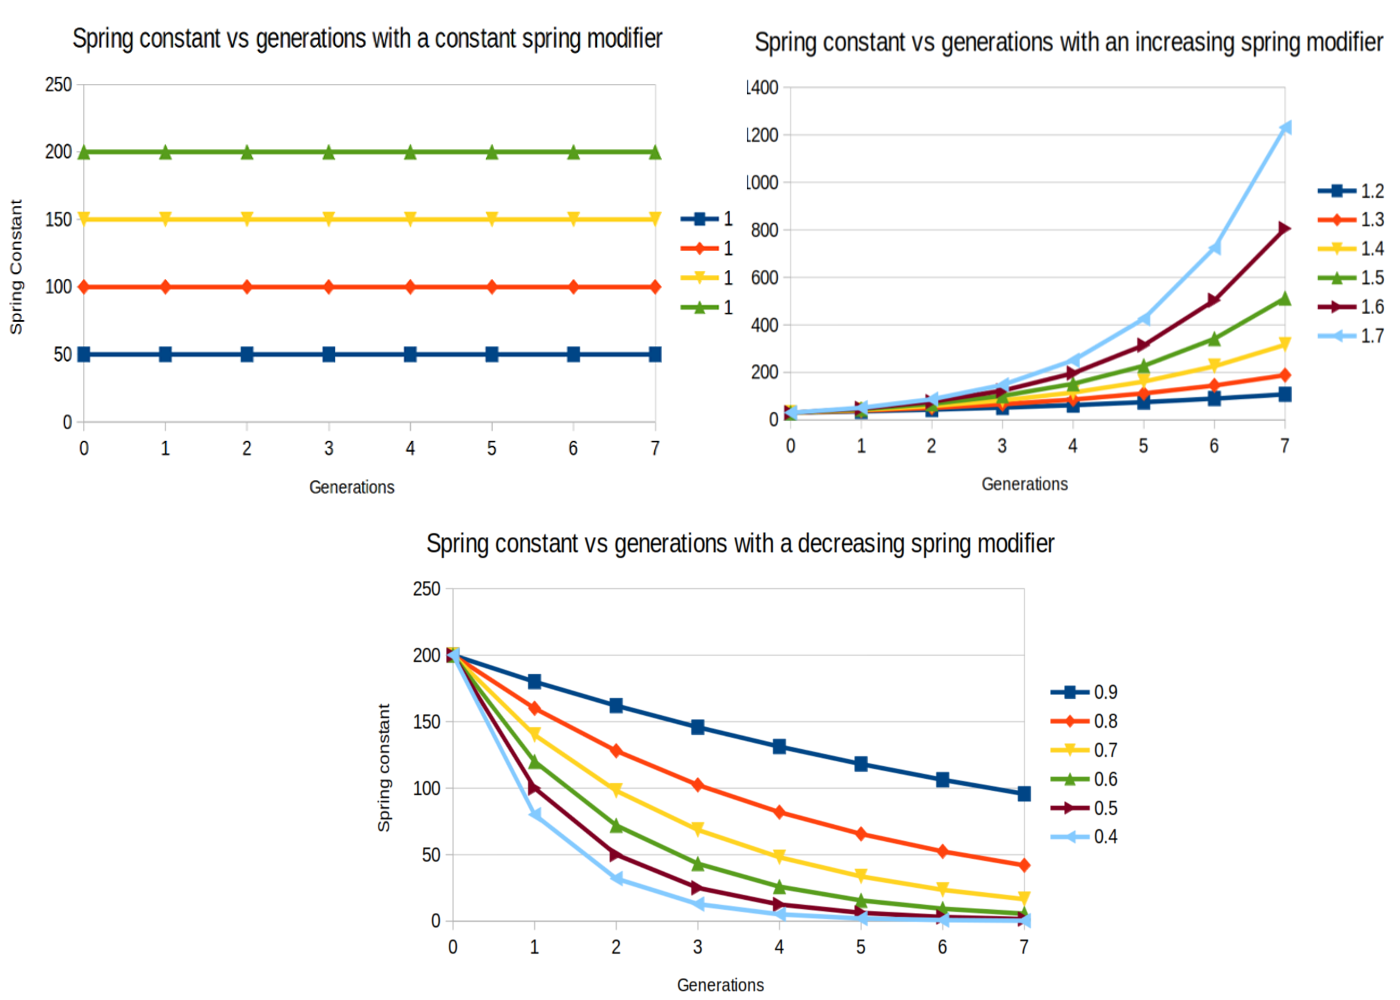
\includegraphics[scale=0.30]{Diagrams/springconstantgraphs.png}
		\caption{Graphs showing the distribution of spring constants dependency on the spring modifier and number of generations.}\label{spring constant graphs}
	}
\end{figure}
\FloatBarrier

\begin{figure}[htbp]
	{\centering
		\vspace{7px}
		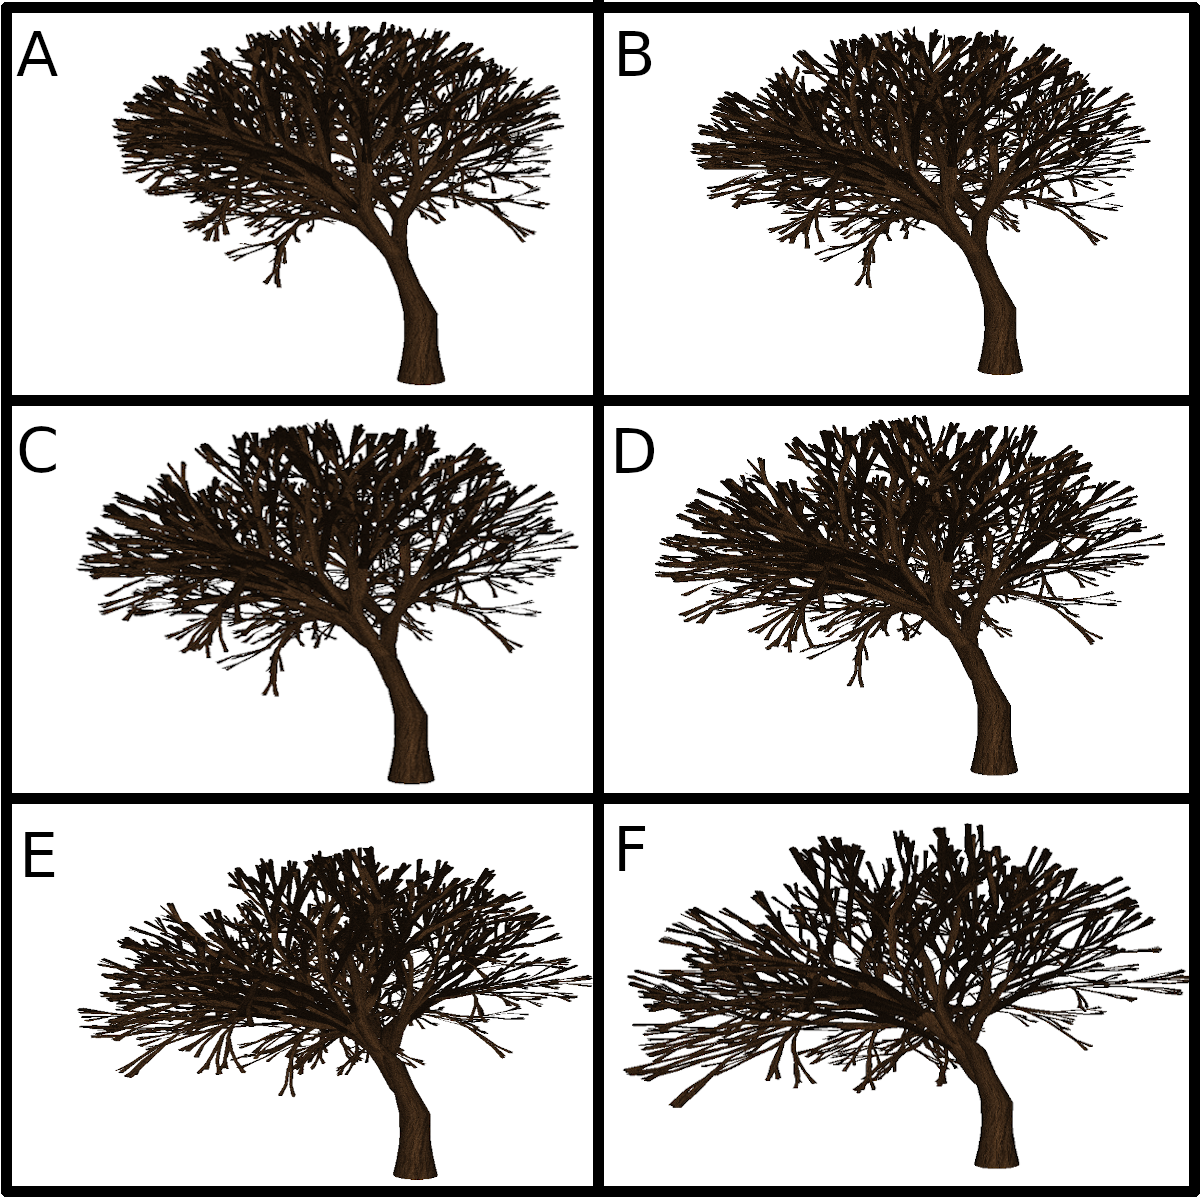
\includegraphics[scale=0.30]{Diagrams/TernaryBranching3_scmod.png}
		\caption{Examples of L-system 3 with gravity applied when changing the spring constant modifier `scmod', when the starting spring constant is set to 30 `scstart = 30'.}\label{increasing scmod}
	}
\end{figure}
\FloatBarrier

\noindent
The L-system below creates the 2D fractal tree that has rendered in three dimensions. It is a 2D tree as it only consists of left and right yaw rotations signified with the `+ and -' symbols without any pitch or roll rotations. In this tree, the rotation `r' is defined as 20$^{\circ}$, the distance `d' is 0.4, and the width `w' is 0.5. The spring constant of the branches is kept at a constant 30.0. This means that all the branches are equally stiff. 

\begin{singlespace}
\begin{equation} \label{2d L-system physics}
\begin{aligned}
	&\textrm{\#n = 6;} \\
	&\textrm{\#define r 20; \#define d 0.4; \#define w 0.5;}\\
	&\textrm{\#w : !(w)Z;}\\
	&\textrm{\#p1 : Z : * : F(d, 30.0)[-(r)Z]F(d, 30.0)[+(r)Z]-(r)Z;}\\
	&\textrm{\#p2 : F(s, x) : * : F(s, x)F(s, x);}
\end{aligned}
\end{equation}
\end{singlespace}

\begin{figure}[htbp]
	{\centering
		\vspace{7px}
		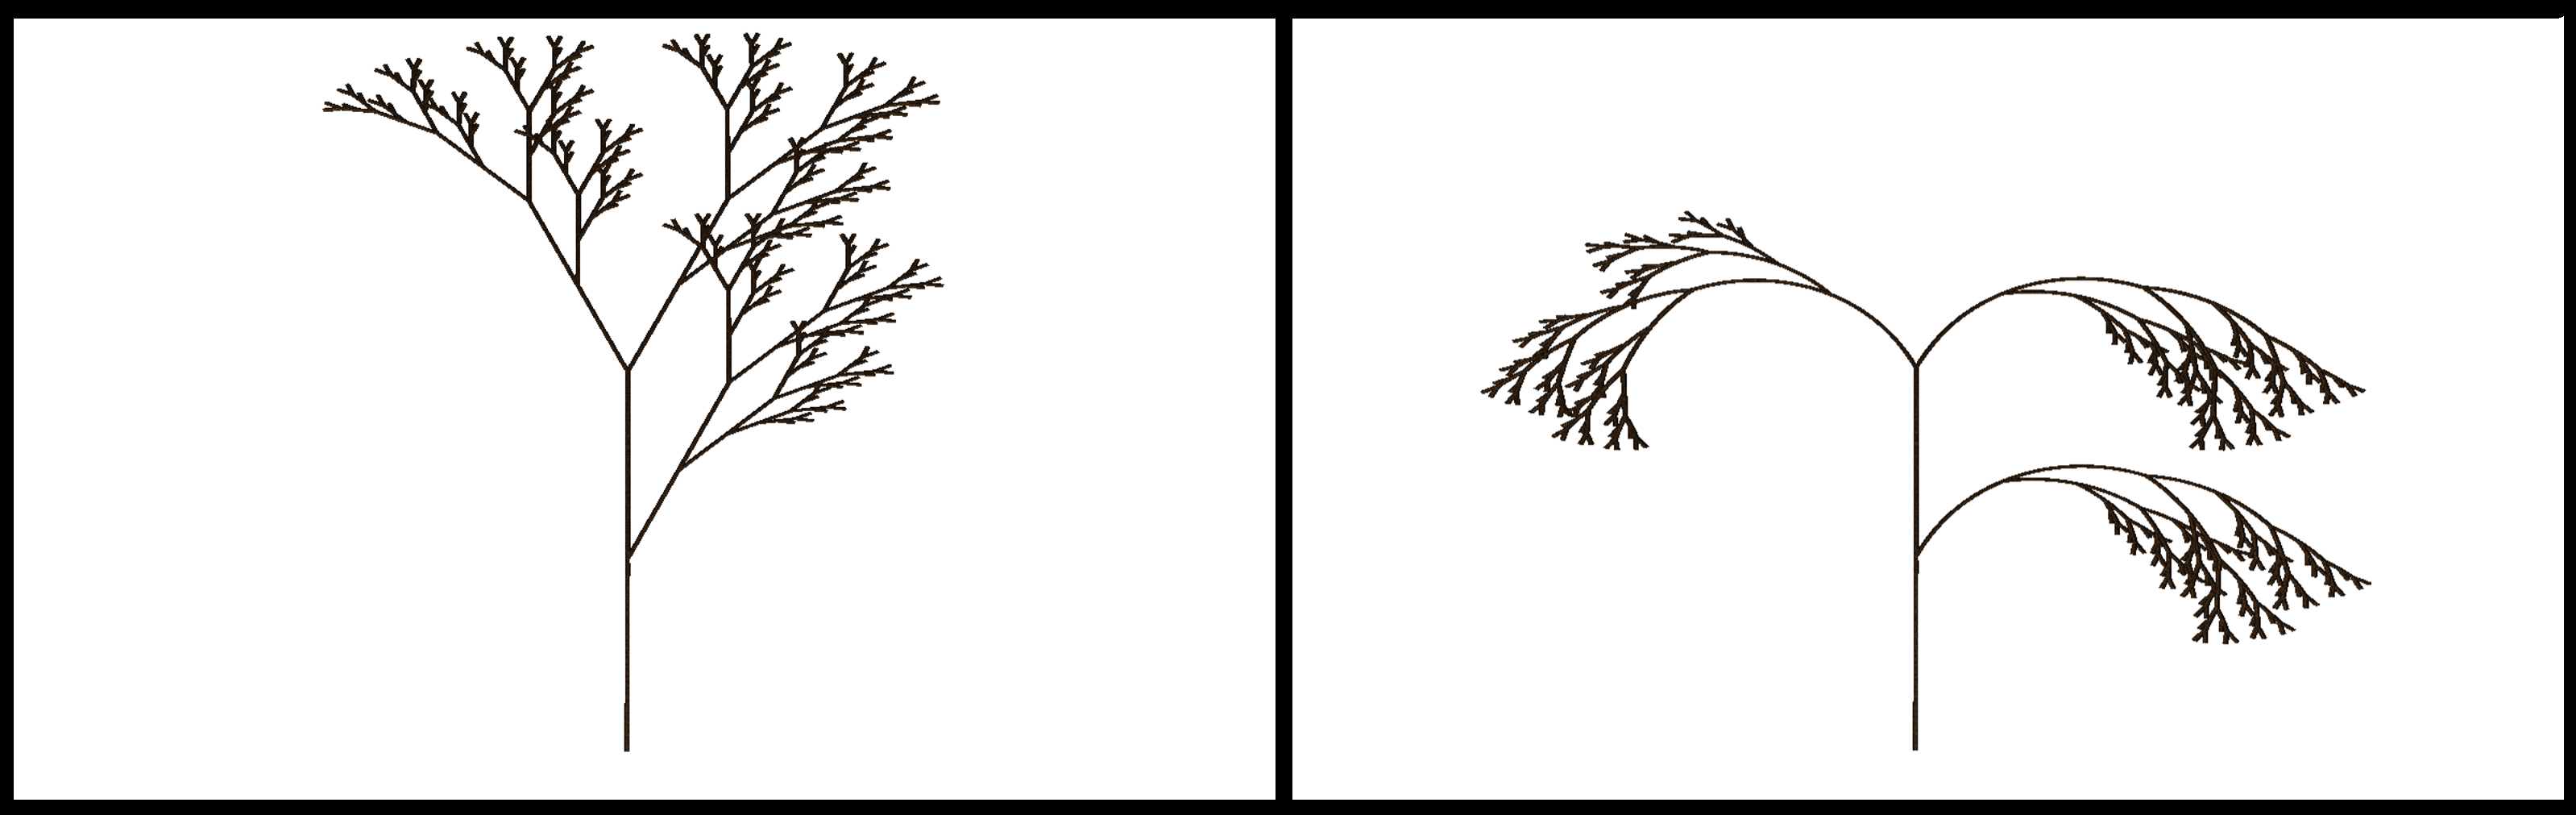
\includegraphics[scale=0.1]{Diagrams/gravityExamples1.png}
		\label{3DAxisFigure} \label{Gravity applied to generated model 1}
		\caption{Examples simulating gravity on a 2D model}
	}
\end{figure}
\FloatBarrier

\noindent
The L-system defined and displayed in figure \ref{Gravity applied to generated model 1} below produces a structure similar to a pine tree. The tree consists of a center branch that branches off in four different directions at several points. Although the structure of the plant is very different from the previously mentioned L-systems, providing the parameters that are necessary for simulations is straightforward, and therefore the simulator can create a convincing effect when gravity or wind is applied. 

\begin{singlespace}
\begin{equation}
\begin{aligned}
	&\textrm{\#n = 5;} \\
	&\textrm{\#object F BRANCH; \#object X SPHERE;}\\
	&\textrm{\#define r 25.7; \#define d 0.5; \#define w 1;}\\
	&\textrm{\#define scstart 30; \#define scmod 1.0;}\\
	&\textrm{\#w : !(1.707)X;}\\
	&\textrm{\#p1 : X : * : F(d, scstart)[!(w)/(r)+(r)X][!(w)-(r)X][!(w)$\land$(r)X][!(w)\&(r)X]!(w)F(d, scstart)X;}\\
	&\textrm{\#p2 : F(s, x) : * : F(s, x * scmod)F(s, x * scmod);}
\end{aligned}
\end{equation}
\end{singlespace}

\begin{figure}[htbp]
	{\centering
		\vspace{7px}
		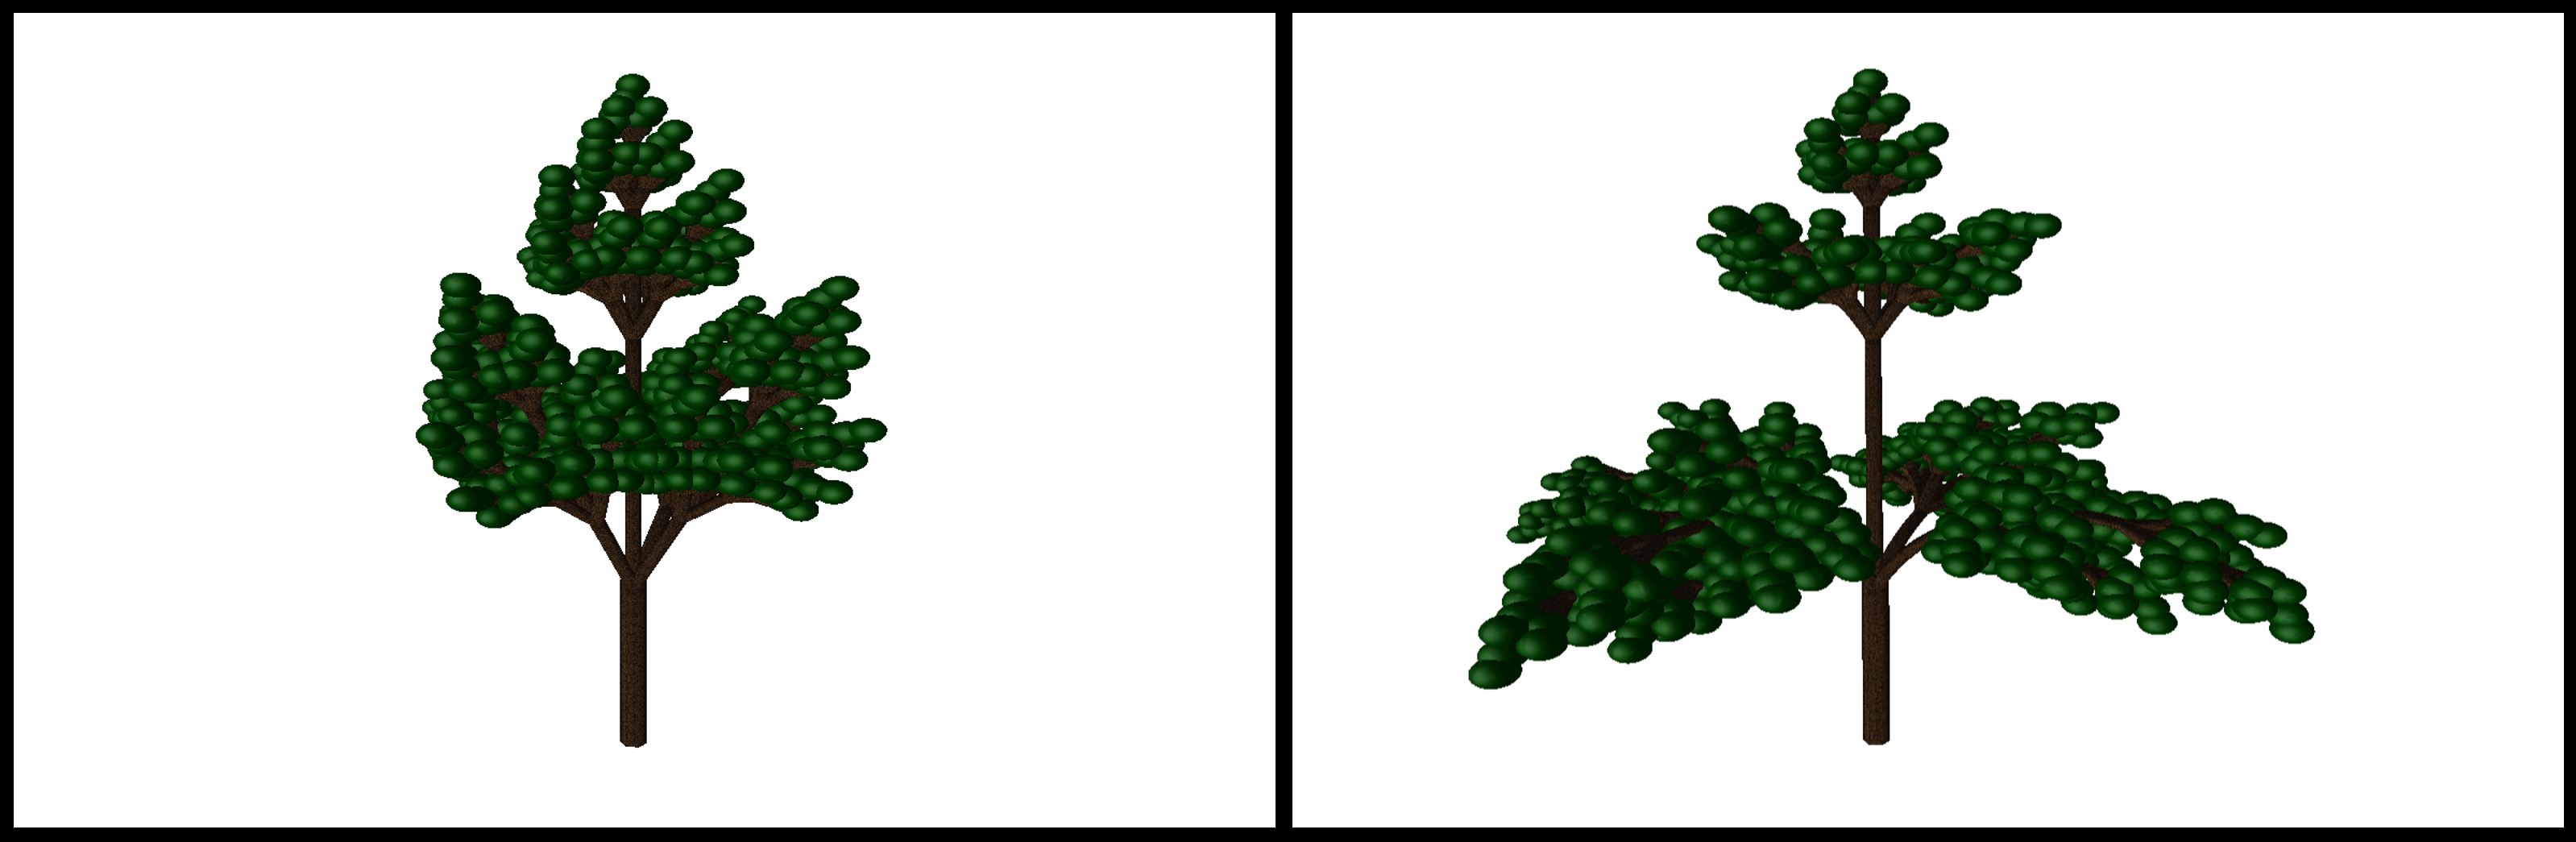
\includegraphics[scale=0.1]{Diagrams/gravityExamples2.png}
		\label{3DAxisFigure} \label{Gravity applied to generated model 1}
		\caption{Simulating gravity on a simple pine tree model.}
	}
\end{figure}
\FloatBarrier

\noindent
In figure \ref{Wind applied to generated model}, the same L-system seen in \ref{Gravity applied to generated model 1} is used; however, the interpreter has been instructed not to render the green spheres at the ends of branches, to see the branching structure better. Instead of gravity, the simulator is showing the effect of wind coming from the right-hand side of the tree. Each image is a timestep showing a pronounced effect of wind on the plant. In a simulation within a video game or 3D application, the wind would be simulated to a lesser extent; however, it would result in a similar movement and rustling of branches.

\begin{figure}[htbp]
	{\centering
		\vspace{7px}
		\includegraphics[scale=0.3]{Diagrams/windExample.png}
		\label{3DAxisFigure} \label{Wind applied to generated model}
		\caption{Simulating wind on a simple pine tree model}
	}
\end{figure}
\FloatBarrier

\noindent
The examples and tests in this chapter show that the parametric L-system can intuitively affect the look of a plant. Parameters can also be used to describe certain aspects of the plants' behaviour when simulated. The parameters can directly affect the simulation, such as the spring constant or spring constant modifier parameters. Additionally, parameters can affect the simulation indirectly with the length or width of branches, which ultimately affect the weight or center of gravity of a branch. Using both the direct and indirect parameters means that the resulting simulation is affected by the look of the plant. Additionally, this gives the user the ability to adjust the plant's behaviour in a way that does not affect its visual appearance. 

The rewriting mechanism of the L-system makes it well suited for providing and manipulating the plants' physical information.  It is possible to use the rewriting mechanism to change a branches' spring constant depending on the number of times that branch has been rewritten. The trees skeletal structure generated by the turtle graphics interpreter makes for a very straightforward particle physics system to simulate each branch of the generated structure. 





\chapter{Discussion and Conclusions}
This thesis investigated whether a procedural generation system can produce both the model and physical properties necessary to render and simulate realistic looking plant-life. The parametric L-system provides a way of defining the structure of a plant as well as parameters that can represent additional information such as the physical properties of the plant. The parameters can be manipulated during the rewriting process to provide multiple different effects, discussed in chapter \ref{results chapter}, such as the width of a tree's branch increasing exponentially with the number of generations. The parametric L-system is a compelling tool for the procedural generation of plant-life as it can produce realistic looking plant structures very quickly and efficiently. In modern 3D applications, a large part of what users perceive as realistic has to do with the movement and motion of objects within a scene. For instance, detailed tree model will appear unrealistic if it is completely motionless in the middle of a storm. Having a single procedural generation system that not only creates the plant model but can provide the skeletal structure and physical attributes it is very convenient as it encapsulates the entire description in one place.

The implementation of the procedural generator for this thesis has two major systems; the L-system rewriter and the interpreter. The rewriter and the interpreter operate independently of one another, however to create the desired result they must both cooperate. Each system has a level of complexity that relies on the other. For instance, a rewriter with many sophisticated features will provide more information to the interpreter; therefore, the interpreter can follow the instructions precisely to produce the desired result. Conversely, a simple rewriter with few features will provide less information to the interpreter, and the interpreter will then have to make more assumptions and do more work to achieve the same result. For the procedural generation system to be effective, the L-system grammar cannot become so complicated that it is unreasonabily difficult to write an L-system for a given plant. It is also limiting to create an L-system that is overly simplistic, such as a DOL-system, as the plant may become too dependant on the interpreter, and become inflexible. It can be challenging to determine where the line of complexity should lie between the rewriter and the interpreter. Depending on the L-systems' representation, there may be a need for emphasis on one side rather than the other. For the implementation in this thesis, the parametric L-system focuses more on the complexity within the rewriter. Having features like parameters, stochastic rules, and conditions mean that the L-system is very powerful, and can provide a large portion of information to the interpreter for both rendering and simulating plants. However, this does have a drawback that the L-system becomes challenging to write and understand.

Although writing the L-systems may be more challenging, changing the look of a plant actually becomes more straightforward. As shown in chapter \ref{results chapter}, changing parameters such as the angle, width, or spring constant of a branch can have a dramatic effect on the overall look of the plant without having to change the structure of the L-system at all. This is further improved with features like stochastic rules and random ranges, which makes it possible to produce models with variation in the structure. These features could be used by artists to create many different variations of the same family of plant-life in a matter of seconds.

Prompts can also be provided to the interpreter to render particular objects or effects by using the \#object declaration. Examples of these features can be seen in chapter \ref{l-system chapter}. This allows an L-system to provide specific information to the interpreter without the L-system dictating how it should be interpreted. The advantage of this approach is the L-system rewriter does not need to change, regardless of the interpretation. Additionally, the rewriting process is kept independent of the interpretation.

There are several ways the creation of plants using an L-system can be made more accessible for those who are not comfortable with writing L-systems. One improvement might be to create a tool where a user can edit the L-system and have its representation reflected immediately as a generated and simulated plant. This will give a user immediate feedback about whether they are getting the desired outcome. This can be built to animate the plant in real-time to see how it would react to different forces like gravity or wind. A different option may be to have a large number of predefined L-systems and only give the user control over manipulating the parameters of the L-system. This may give the user less control over the `species' of the plant but will make it much easier to modify the plant and get a result quickly.

This thesis found that it is possible to use and L-system to provide the information necessary to simulate the effect of gravity and wind on a procedurally generated plant. Using the L-system to specify features such as the width, length, and bending coefficient of branches makes it relatively straightforward to implement a physical simulation within the interpreter. In the same way that there is a trade-off between the rewriter and interpreter for procedural generation, the features provided for simulation makes the L-system more cumbersome and difficult to read. This begs the question as to what features should be provided by the L-system and which should be left up to the interpreter to decide? For instance, should the density of the plant material be defined by each branch segment within the L-system, or should it be chosen by the interpreter? 


\printglossary[type=\acronymtype]
\printglossary

\begin{appendices}
\section{Appendix 1}

\section{Bibliography}
\bibliography{chapters/ref}
\bibliographystyle{apalike}



\end{appendices}



\end{document}



